% Sumber LaTeX untuk buku ``Metode Aljabar'' dalam bahasa Mandarin
% Hak Cipta 2018  Wen-Wei Li.
% Izin diberikan untuk menyalin, mendistribusikan, dan/atau memodifikasi
% dokumen ini berdasarkan ketentuan Creative Commons
% Attribution 4.0 International (CC BY 4.0)
% http://creativecommons.org/licenses/by/4.0/

% Untuk disertakan
\chapter{Teori Modul}\label{sec:modules}
Menurut cara perkalian skalarnya, modul dibedakan menjadi modul kiri dan modul kanan. Secara kasar, modul kiri $M$ atas gelanggang $R$ dapat dianalogikan dengan ruang vektor: $M$ sendiri merupakan grup terhadap penjumlahan dan dilengkapi perkalian skalar kiri oleh $R$, yaitu $R \times M \to M$. Dari sudut pandang ini, ruang vektor adalah modul atas medan, sedangkan grup abelian tidak lain adalah $\Z$-modul.

Modul merupakan struktur yang lentur dan sangat luas kegunaannya dalam matematika; sebagai contoh,
\begin{inparaenum}[(a)]
	\item teorema struktur modul terbangkitkan hingga atas daerah ideal utama mencakup klasifikasi grup abelian terbangkitkan hingga serta teori bentuk kanonik transformasi linear;
	\item kategori modul atas gelanggang $R$ sekaligus merupakan contoh baku dalam teori kategori dan pola dasar awal bagi aljabar homologis;
	\item hasil kali tensor modul memberikan contoh yang sangat baik bagi kategori monoidal simetris.
\end{inparaenum}
Jika dikembangkan lebih jauh, pembahasan dalam bab ini mengenai barisan eksak serta modul projektif dan injektif mengarah ke teori gelanggang komutatif dan aljabar homologis; sementara itu, pembahasan modul semisederhana dan modul tak teruraikan secara alami menuju teori representasi grup dan aljabar. Ke arah mana pun kita melangkah, hasil kali tensor merupakan alat yang wajib dikuasai dan salah satu pokok utama dalam pengantar teori modul.

Mulai bab ini, sudut pandang teori kategori akan diperkenalkan secara bertahap. Di satu pihak, sudut pandang ini menata sifat-sifat modul secara efisien, termasuk berbagai fungtor antarkategori modul dan transformasi natural di antaranya. Di pihak lain, ini memberi kesempatan kepada pembaca untuk membiasakan diri dengan gagasan teori kategori: konsep seperti fungtor adjoin, limit, sifat universal, dan kategori monoidal semuanya memperoleh tempat yang sesuai dalam teori modul, menunjukkan bahwa perangkat abstrak ini bersifat alami sekaligus perlu.

\begin{wenxintishi}
	Hasil kali tensor adalah salah satu pokok kunci teori modul. Untuk mencakup keadaan umum, kita akan membangun teori umum dalam konteks bimodul; karena itu, perumusannya tampak lebih rumit. Pembaca dapat memulai dari kasus gelanggang komutatif; lihat Contoh \ref{eg:bimodule-comm}. Kita akan memakai bahasa kategori monoidal dan fungtor monoidal untuk menyatakan berbagai sifat hasil kali tensor. Pembaca tidak perlu menelaah setiap definisi teori kategori yang terkait satu demi satu, tetapi hendaknya benar-benar memahami gagasan pokok kategori monoidal: kategori monoidal adalah kategori yang dilengkapi ``hasil kali tensor'' $\otimes$ beserta berbagai isomorfisme kendala, sedangkan fungtor monoidal adalah fungtor yang mempertahankan $\otimes$ hingga isomorfisme natural.
	
	Pembahasan bab ini tentang barisan eksak, modul projektif/injektif, dan syarat rantai dapat dipandang sebagai pemanasan sebelum memasuki teori gelanggang komutatif dan aljabar homologis; pembahasannya memang hanya pengantar. Kerangka umum yang tepat untuk mempelajari konsep-konsep tersebut adalah kategori abelian; kategori modul kiri atas gelanggang $R$ merupakan contoh khas kategori abelian.
\end{wenxintishi}

\section{Konsep Dasar}
Dari sudut pandang formal, modul adalah grup aditif yang dilengkapi suatu keluarga operator perkalian. Ingat kembali asumsi kita: grup aditif berarti grup abelian $A$ dengan operasi biner yang ditulis $+$, unsur identitas yang ditulis $0$, dan invers aditif unsur $a \in A$ yang ditulis $-a$.

\begin{definition}\index{modul@modul (module)}
	Misalkan $R$ suatu gelanggang. Sebuah \emph{modul} kiri atas $R$ terdiri atas data berikut:
	\begin{itemize}
		\item grup aditif $(M, +)$;
		\item peta $R \times M \to M$, yang ditulis $(r, m) \mapsto r \cdot m = rm$ (perkalian kiri), dengan sifat-sifat berikut:
		\begin{align*}
			r(m_1 + m_2) &= rm_1 + rm_2, \qquad r \in R, \; m_1, m_2 \in M, \\
			(r_1 + r_2)m &= r_1 m + r_2 m, \qquad r_1, r_2 \in R, \; m \in M, \\
			(r_1 r_2)m & = r_1 (r_2 m), \\
			1_R \cdot m & = m.
		\end{align*}
	\end{itemize}
	Jika perkalian kiri dalam definisi diganti dengan perkalian kanan $(m, r) \mapsto mr$, dan syaratnya diganti dengan $m(r_1 r_2) = (mr_1)r_2$ dan seterusnya, konsep yang diperoleh disebut modul kanan atas $R$. Biasanya cukup dikatakan bahwa $M$ adalah modul kiri atau modul kanan atas $R$.
\end{definition}

Sebagaimana dalam kasus ruang vektor yang telah dikenal, operasi $R \times M \to M$ juga disebut perkalian skalar oleh $R$. Dari aksioma-aksioma di atas mudah diturunkan sifat-sifat berikut dalam modul kiri $M$ atas $R$:
\begin{equation}\label{eqn:multiples-in-module}\begin{aligned}
	0 \cdot m & = 0, \quad m \in M, \\
	(-1_R) \cdot m & = -m, \\
	(n \cdot 1_R) \cdot m & = nm = \underbracket{m + \cdots + m}_{n\text{ suku}}, \quad n \in \Z_{\geq 0}, \\
	(-n \cdot 1_R) \cdot m & = -(nm).
\end{aligned}\end{equation}
Dengan demikian, ungkapan berbentuk $n \cdot m$ ($n \in \Z$) tidak ambigu: ungkapan itu dapat dipandang sebagai operasi kelipatan dalam $(M,+)$ maupun sebagai aksi perkalian oleh $n \cdot 1_R \in R$. Kasus modul kanan serupa.

\begin{remark}\label{rem:module-multiplication}
	Menurut Contoh \ref{eg:End-ring}, himpunan endomorfisme $\End(M)$ dari sebarang grup aditif $(M, +)$ memiliki struktur gelanggang alami; perkaliannya adalah komposisi homomorfisme dan penjumlahannya adalah penjumlahan homomorfisme ``titik demi titik''. Memberikan struktur modul kiri atas $R$ pada $(M,+)$ ekuivalen dengan memberikan homomorfisme gelanggang
	\begin{align*}
		R & \longrightarrow \End(M) \\
		r & \longmapsto [m \mapsto rm],
	\end{align*}
	sedangkan memberikan struktur modul kanan atas $R$ ekuivalen dengan memberikan homomorfisme gelanggang
	\begin{align*}
		R^\text{op} & \longrightarrow \End(M) \\
		r & \longmapsto [m \mapsto mr].
	\end{align*}
	Dari sini segera diperoleh
	\begin{center}
		modul kiri atas $R$ = modul kanan atas $R^\text{op}$.
	\end{center}
	Untuk gelanggang komutatif $R$, tidak perlu dibedakan modul kiri dan kanan; kita cukup menyebutnya $R$-modul.
\end{remark}

\begin{example}
	Setiap gelanggang $R$, dengan perkalian kiri pada dirinya sendiri, merupakan modul kiri atas $R$; dengan perkalian kanan, ia merupakan modul kanan atas $R$.
\end{example}

\begin{example}\label{eg:Z-modules}
	Modul atas gelanggang bilangan bulat $\Z$ tidak lain adalah grup aditif. Hal ini karena hanya ada satu aksi perkalian $\Z$ pada $M$, yakni yang diberikan oleh \eqref{eqn:multiples-in-module}. Jadi, teori grup abelian dapat dipandang sebagai salah satu cabang teori modul.
\end{example}

\begin{definition}\label{def:submodule}\index{submodul@submodul (submodule)}
	Misalkan $M$ suatu modul kiri atas $R$. Jika subhimpunan $M' \subset M$ memenuhi
	\begin{itemize}
		\item ketertutupan terhadap penjumlahan: $M'$ adalah subgrup dari grup aditif $(M, +)$,
		\item ketertutupan terhadap perkalian skalar: untuk setiap $r \in R$ dan $m \in M'$, berlaku $rm \in M'$,
	\end{itemize}
	maka $M'$ disebut \emph{submodul} dari $M$. Definisi submodul bagi modul kanan serupa.

	Jika modul kiri atau kanan $M$ tidak mempunyai submodul selain $\{0\}$ dan $M$ sendiri, serta $M \neq \{0\}$, maka $M$ disebut \emph{modul sederhana}.\index{modul!sederhana (simple)}
\end{definition}

Dalam uraian berikut, anggap $M$ sebagai modul kiri atas $R$. Misalkan $\{M_i: i \in I\}$ suatu keluarga submodul dari $M$. Maka jumlahnya
\[ \sum_{i \in I} M_i := \left\{ 
	\begin{array}{ll}
		m_{i_1} + \cdots + m_{i_r} : & r \in \Z_{\geq 1}, \; i_1, \ldots, i_r \in I \\
		& \forall 1 \leq k \leq r, \; m_{i_k} \in M_{i_k}
	\end{array} \right\} \]
(dengan konvensi bahwa jumlah kosong adalah $\{0\}$) dan irisannya (untuk $I \neq \emptyset$)
\[ \bigcap_{i \in I} M_i \]
tetap merupakan submodul. Jika $S$ adalah subhimpunan dari $M$, kita dapat mendefinisikan submodul $\lrangle{S}$ yang dibangkitkan oleh $S$ sebagai submodul terkecil dalam $M$ yang memuat $S$, yakni
\[ \lrangle{S} := \bigcap_{\substack{M': \text{submodul} \\ M' \supset S}} M'. \]
Jika $S$ adalah himpunan satu elemen $\{x\}$, maka $\lrangle{S} = \lrangle{x}$ memiliki deskripsi langsung $Rx := \{rx : r \in R\}$. Secara umum, mudah diperiksa bahwa $\lrangle{S} = \sum_{x \in S} Rx \subset M$. Modul yang dapat ditulis dalam bentuk $Rx$ disebut \emph{modul siklik}; bila $R=\Z$, modul siklik tidak lain adalah grup siklik.

Untuk modul kanan atas $R$, kita dapat mendefinisikan submodul $xR$ dan seterusnya dengan cara yang sama; rinciannya tidak diulangi.

\begin{example}
	Gelanggang $R$ memiliki struktur modul kiri dan modul kanan alami atas dirinya sendiri melalui perkaliannya. Dengan membandingkan definisi submodul dan ideal pada \ref{def:ideals}, diperoleh
	\begin{center}
		submodul dari $R$ sebagai modul kiri atas $R$ = ideal kiri dari $R$, \\
		submodul dari $R$ sebagai modul kanan atas $R$ = ideal kanan dari $R$.
	\end{center}
	Teori modul sendiri dibangun di atas konsep gelanggang; kelak akan kita lihat bagaimana sudut pandang $R$-modul dapat digunakan untuk menyimpulkan sifat-sifat teori gelanggang dari $R$.
\end{example}

\begin{definition}\index{homomorfisme}
	Misalkan $M_1$, $M_2$ modul kiri atas $R$. Sebuah peta $\varphi: M_1 \to M_2$ disebut \emph{homomorfisme modul} dari $M_1$ ke $M_2$ jika memenuhi
	\begin{itemize}
		\item $\varphi$ adalah homomorfisme grup aditif: untuk semua $x, y \in M_1$, berlaku $\varphi(x+y)=\varphi(x) + \varphi(y)$,
		\item $\varphi$ mempertahankan perkalian skalar: untuk semua $r \in R$ dan $x \in M_1$, berlaku $\varphi(rx) = r\varphi(x)$.
	\end{itemize}
	Peta identitas jelas merupakan homomorfisme, dan komposisi homomorfisme $\varphi: M_1 \to M_2$, $\psi: M_2 \to M_3$, yakni $\psi\varphi: M_1 \to M_3$, tetap merupakan homomorfisme. Dengan demikian diperoleh kategori modul kiri atas $R$, yaitu $R\dcate{Mod}$, beserta konsep isomorfisme, automorfisme, dan sebagainya. Kategori modul kanan atas $R$ didefinisikan secara serupa dan ditulis $\cated{Mod}R$.\index{isomorfisme}

	Untuk homomorfisme $\varphi$ di atas, definisikan \emph{kernel}-nya, atau kernel nolnya, sebagai $\Ker(\varphi) := \{x \in M_1 : \varphi(x)=0 \}$, dan \emph{bayangan}-nya sebagai $\Image(\varphi) := \{\varphi(x) : x \in M_1\}$. Keduanya masing-masing merupakan submodul dari $M_1$ dan $M_2$.\index{kernel}
\end{definition}

Seperti pada kasus monoid dan gelanggang, homomorfisme $\varphi: M_1 \to M_2$ adalah isomorfisme jika dan hanya jika $\varphi$ bijektif. Dalam hal itu, peta inversnya $\varphi^{-1}: M_2 \to M_1$ juga merupakan homomorfisme modul: cukup terapkan $\varphi^{-1}$ pada persamaan-persamaan yang dipenuhi $\varphi$ dalam definisi.

\begin{remark}\label{rem:Mod-cat-preadditive}
	Seperti untuk grup abelian atau $\Z$-modul, bagi sebarang modul kiri (atau kanan) $M, M'$ atas $R$, himpunan homomorfisme $\Hom_{R\dcate{Mod}}(M, M') =: \Hom_R(M, M')$ membentuk grup aditif: untuk sebarang $\phi, \psi \in \Hom_R(M, M')$, definisikan
	\[ \phi + \psi := [m \mapsto \phi(m) + \psi(m) ] \in \Hom_R(M, M'). \]
	Unsur nol dari grup $\Hom_R(M, M')$ adalah \emph{morfisme nol} $\forall m \mapsto 0$. Selain itu, operasi komposisi homomorfisme
	\begin{align*}
		\Hom_R(M', M'') \times \Hom_R(M, M') & \longrightarrow \Hom_R(M, M'') \\
		(\phi, \psi) & \longmapsto \phi \psi
	\end{align*}
	merupakan peta $\Z$-bilinear, yakni:
	\[ \phi(\psi_1 + \psi_2) = \phi\psi_1 + \phi\psi_2, \quad (\phi_1 + \phi_2)\psi = \phi_1\psi + \phi_2\psi. \]

	Dari sini terlihat pula bahwa himpunan endomorfisme $\End_R(M)$ dari $M$ memiliki struktur gelanggang alami, dengan perkalian yang diberikan oleh komposisi. Sekarang tinjau modul kanan $M$ atas $R$. Modul $M$ memperoleh struktur modul kiri alami atas $D := \End_R(M)$ sebagai berikut:
	\begin{align*}
		D \times M & \longrightarrow M \\
		(\phi, m) & \longmapsto \phi(m).
	\end{align*}
	Pokoknya adalah bahwa aksi perkalian $D$ ``komutatif'' dengan aksi $R$, dalam arti $\phi(mr)=\phi(m)r$. Kelak kita akan melihat kegunaan struktur ini; lihat Konvensi \ref{con:Hom-assoc}, \ref{con:left-right-End}.
\end{remark}

Menurut Catatan \ref{rem:module-multiplication}, kategori $R\dcate{Mod}$ ekuivalen dengan $\cated{Mod}R^\text{op}$. Demi kemudahan, selanjutnya kita menetapkan gelanggang $R$ dan hanya membahas modul kiri.

Sekarang kita tinjau struktur hasil bagi modul. Singkatnya, memberikan suatu relasi ekuivalensi $\sim$ pada modul kiri $M$ yang ``mempertahankan struktur modul'' ekuivalen dengan memberikan suatu submodul $N$; kaitan keduanya adalah
\[ x \sim y \iff x-y \in N. \]
Rinciannya dapat dilihat pada pembahasan \ref{sec:homomorphism}. Di sini kita hanya menjelaskan cara membangun modul hasil bagi $M \twoheadrightarrow M/N$ dari submodul $N \subset M$ yang diberikan. Pertama, sebagai grup aditif, hasil bagi $(M/N, +)$ sudah terdefinisi: unsur-unsurnya adalah koset aditif berbentuk $x+N$, dengan operasi biner $(x+N) + (y+N) = x+y + N$. Yang tersisa adalah menambahkan perkalian skalar oleh $R$.

\begin{definition}\index{hasil bagi}
	Misalkan $N \subset M$ suatu submodul. Pada grup hasil bagi aditif $M/N$, definisikan struktur modul kiri atas $R$ dengan
	\[ r (x+N) = rx + N, \qquad r \in R, \; x \in M. \]
	Maka peta hasil bagi $M \to M/N$ merupakan homomorfisme modul, dan $M/N$ disebut \emph{modul hasil bagi} dari $M$ oleh $N$.
\end{definition}

Modul hasil bagi memiliki sejumlah sifat formal yang serupa dengan grup hasil bagi, gelanggang hasil bagi, dan sebagainya. Berikut ringkasannya. Pembuktiannya serupa dengan kasus grup dan bahkan lebih sederhana karena tidak perlu mempertimbangkan masalah komutativitas.

\begin{proposition}\label{prop:1st-homomorphism-module}
	Modul hasil bagi $M \twoheadrightarrow M/N$ memenuhi sifat universal berikut: untuk setiap homomorfisme modul $\varphi: M \to M'$, jika $N \subset \Ker(\varphi)$, maka terdapat tepat satu homomorfisme $\bar{\varphi}: M/N \to M'$ sehingga diagram
	\[ \begin{tikzcd}
		M \arrow[rd, "\varphi"'] \arrow[r] & M/N \arrow[d, "{\exists! \; \bar{\varphi}}"]\\
		& M'
	\end{tikzcd}\]
	komutatif.
\end{proposition}
\begin{proof}
	Satu-satunya pilihan adalah $\bar{\varphi}(x + N) = \varphi(x)$; mudah diperiksa bahwa peta ini terdefinisi dengan baik.
\end{proof}

\begin{proposition}\label{prop:quotient-image-module}
	Misalkan $\varphi: M_1 \to M_2$ suatu homomorfisme modul. Maka $\varphi$ menginduksi isomorfisme $\bar{\varphi}: M_1/\Ker(\varphi) \rightiso \Image(\varphi)$ yang memetakan $m + \Ker(\varphi)$ ke $\varphi(m)$.
\end{proposition}
\begin{proof}
	Terapkan Proposisi \ref{prop:1st-homomorphism-module}.
\end{proof}

\begin{proposition}\label{prop:2nd-homomorphism-module}
	Misalkan $\varphi: M_1 \to M_2$ suatu homomorfisme modul surjektif. Maka terdapat bijeksi
	\[ \begin{tikzcd}[row sep=tiny]
		\left\{ \text{submodul }  N_2 \subset M_2  \right\} \arrow[r, "1:1"] & \left\{ \text{submodul } N_1 \subset M_1 : N_1 \supset \Ker(\varphi)  \right\} \\
		N_2 \arrow[mapsto,r] & \varphi^{-1}(N_2) \\
		\varphi(N_1) & N_1 \arrow[mapsto, l].
	\end{tikzcd} \]
	Bijeksi ini memenuhi $N_2 \subset N'_2 \iff \varphi^{-1}(N_2) \subset \varphi^{-1}(N'_2)$. Selain itu, morfisme komposit $M_1 \xrightarrow{\varphi} M_2 \twoheadrightarrow M_2/N_2$ menginduksi isomorfisme $M_1/\varphi^{-1}(N_2) \rightiso M_2/N_2$.
\end{proposition}
Dengan mengambil $\varphi$ sebagai homomorfisme hasil bagi $M \twoheadrightarrow M/N$, isomorfisme dalam pernyataan dapat ditulis dalam bentuk yang dikenal, $M/N' \rightiso (M/N) \big/ (N'/N)$, dengan $N \subset N'$.
\begin{proof}
	Rutin.
\end{proof}

\begin{proposition}\label{prop:3rd-homomorphism-module}
	Misalkan $M, N$ submodul dari $\mathcal{M}$. Homomorfisme komposit $M \hookrightarrow M+N \twoheadrightarrow (M + N)/N$ menginduksi isomorfisme modul natural
	\begin{align*}
		M/(M \cap N) & \rightiso (M+N)/N, \\
		m + (M \cap N) & \mapsto m + N, \quad m \in M.
	\end{align*}
\end{proposition}
\begin{proof}
	Batasi homomorfisme hasil bagi $\pi: \mathcal{M} \to \mathcal{M}/N$ pada $M$. Bayangannya jelas $\pi(M) = M+N$, sedangkan kernelnya $M \cap \Ker(\pi) = M \cap N$. Dengan menerapkan Proposisi \ref{prop:quotient-image-module}, diperoleh isomorfisme $M/(M \cap N) \rightiso (M+N)/N$ yang memetakan $m + (M \cap N)$ ke $m + N$.
\end{proof}

\begin{definition}\label{def:cokernel}
	Untuk homomorfisme modul $f: M \to M'$, definisikan \emph{kokernel}-nya sebagai $\Coker(f) := M'/\Image(f)$.
\end{definition}
Sifat-sifat lebih lanjut dari kategori modul $R\dcate{Mod}$ akan dipelajari dalam \S\ref{sec:exactseq-module}.

\section{Operasi Dasar pada Modul}\label{sec:mod-operations}
Dalam bagian ini, tetapkan gelanggang $R$ dan anggap semua modul sebagai modul kiri atas $R$. Kasus modul kanan sepenuhnya serupa.

\begin{definition}\label{def:tor-ann}
	Misalkan $M$ suatu $R$-modul.
	\begin{itemize}\index[sym1]{ann@$\text{ann}_M$}
		\item \emph{Anihilator} suatu unsur $x \in M$ didefinisikan sebagai ideal kiri dari $R$ berikut:
		\[ \text{ann}_M(x) := \{r \in R : rx=0 \}. \]
		Jika $\text{ann}_M(x)=\{0\}$, maka $x$ disebut \emph{bebas torsi}; jika tidak, $x$ disebut \emph{unsur torsi}. Modul yang semua unsur tak nolnya bebas torsi disebut \emph{modul bebas torsi}. \index{modul!bebas torsi (torsion-free)}
		\item Anihilator modul $M$ didefinisikan sebagai ideal dua sisi dari $R$ berikut:
		\[ \text{ann}(M) := \left\{r \in R: \forall x \in M, \; rx=0 \right\} = \bigcap_{x \in M} \text{ann}_M(x). \]
		Jika ideal dua sisi $I$ dari $R$ termuat dalam $\text{ann}(M)$, maka $M$ secara alami menjadi modul atas $R/I$: penjumlahannya tetap, sedangkan perkalian skalarnya didefinisikan oleh $(r + I)m = rm$, dengan $(r,m) \in R \times M$.
		\item \emph{Bagian $\mathfrak{a}$-torsi} dari modul $M$ terhadap ideal kanan $\mathfrak{a} \subset R$ didefinisikan sebagai submodul \index[sym1]{$M[\mathfrak{a}]$}
		\[ M[\mathfrak{a}] := \left\{ m \in M: \forall a \in \mathfrak{a}, \; am=0 \right\}. \]
	\end{itemize}
\end{definition}
Istilah-istilah ini akan digunakan dalam \S\ref{sec:PID-module}. Pembaca dipersilakan memeriksa bahwa anihilator $M$, ketika dipandang sebagai modul atas $R/\mathrm{ann}(M)$, otomatis sama dengan $\{0\}$.

Tujuan selanjutnya dalam bagian ini adalah teorema berikut. \index[sym1]{R-Mod@$R\dcate{Mod}$}
\begin{theorem}\label{prop:module-cat-completeness}
	Kategori $R\dcate{Mod}$ lengkap dan kolengkap, serta mempunyai objek nol.
\end{theorem}

Objek nol adalah objek yang sekaligus merupakan objek awal dan objek terminal; lihat Definisi \ref{def:universal-objects}. Untuk kelengkapan dan kekolengkapan, lihat Definisi \ref{def:completeness}; secara eksplisit, kategori $R$-modul mempunyai semua limit kecil. Untuk kata sifat ``kecil'', lihat Definisi \ref{def:U-cat}. Kasus khusus $\Z$-modul, yakni grup abelian, telah digambarkan dalam Contoh \ref{eg:complete-cocomplete}. Pembuktian berikut sekaligus memperkenalkan beberapa notasi baku untuk jumlah langsung dan produk langsung.

\begin{proof}
	Catatan \ref{rem:Mod-cat-preadditive} telah menunjukkan bahwa $R\dcate{Mod}$ adalah kategori-$\cate{Ab}$: artinya, himpunan-$\Hom$ di dalamnya mempunyai struktur grup aditif alami yang membuat komposisi morfisme bilinear. Khususnya, untuk setiap $M$, $M'$ terdapat morfisme nol $0: M \to M'$ yang memetakan setiap unsur ke $0$. Berikutnya kita membangun berbagai limit secara berurutan.

	\begin{asparaenum}
		\item Objek nol dalam kategori $R\dcate{Mod}$ adalah modul nol $\{0\}$, yang sering cukup ditulis $0$. Struktur modul padanya hanya mungkin diberikan oleh $r \cdot 0 = 0$. Jelas bahwa semua morfisme dari atau ke modul nol tepat merupakan morfisme nol; jadi, modul ini memang objek nol dalam kategori $R\dcate{Mod}$.

		\item Selanjutnya kita membangun produk dan koproduk dalam $R\dcate{Mod}$. Misalkan $I$ suatu himpunan kecil dan $\{M_i : i \in I\}$ suatu keluarga $R$-modul. Definisikan \emph{produk} (atau \emph{produk langsung}) $\prod_{i \in I} M_i$ sebagai
		\begin{align*}
			\prod_{i \in I} M_i & := \left\{ (m_i)_{i \in I} : \forall i \in I, \; m_i \in M_i \right\}, \\
			(m_i)_{i \in I} + (m'_i)_{i \in I} & := (m_i + m'_i)_{i \in I}, \\
			r(m_i)_{i \in I} & := (rm_i)_{i \in I}, \quad r \in R.
		\end{align*}
		Jelas bahwa $\prod_{i \in I} M_i$ merupakan $R$-modul, dengan unsur nol yang diberikan oleh $\forall i \in I, \; m_i = 0$. Modul ini dilengkapi keluarga homomorfisme proyeksi
		\begin{align*}
			p_j: \prod_{i \in I} M_i & \longrightarrow M_j, \qquad j \in I \\
			(m_i)_{i \in I} & \longmapsto m_j.
		\end{align*}

		Definisikan \emph{koproduk}-nya (yang lazim disebut \emph{jumlah langsung}) sebagai \index{jumlah langsung@jumlah langsung (direct sum)}
		\begin{gather*}
			\bigoplus_{i \in I} M_i := \left\{ (m_i)_{i \in I} \in \prod_{i \in I} M_i : \text{hanya berhingga banyak } m_i \neq 0 \right\}.
		\end{gather*}
		Mudah dilihat bahwa $\bigoplus_{i \in I} M_i$ merupakan submodul dari $\prod_{i \in I} M_i$. Modul ini dilengkapi keluarga homomorfisme inklusi
		\begin{align*}
			\iota_j: M_j & \longrightarrow \prod_{i \in I} M_i \\
			m_j & \longmapsto (m_i)_{i \in I}, \quad m_i :=
			\begin{cases}
				m_j, & i=j, \\
				0, & i \neq j.
			\end{cases}
		\end{align*}

		Jika setiap $M_i = M$, produk langsung dan jumlah langsung yang bersangkutan sering ditulis $M^I$ dan $M^{\oplus I}$. Bila $I=\{1, \ldots, n\}$, kita sering memakai notasi $M_1 \times \cdots \times M_n$ dan $M_1 \oplus \cdots \oplus M_n$; keduanya jelas merupakan $R$-modul yang sama. Pembaca dapat pula melihat pembahasan biproduk dalam \ref{def:biproduct}. Kembali ke kasus $I$ umum, kita sekarang memeriksa sifat-sifat kategoris produk dan koproduk dari \S\ref{sec:limits}.

		Diberikan modul $M$ dan keluarga homomorfisme $\phi_j: M \to M_j$, kita menginginkan tepat satu $\phi: M \to \prod_{i \in I} M_i$ yang membuat diagram berikut komutatif untuk setiap $j \in I$:
		\[ \begin{tikzcd}
			M \arrow[rd, "\phi_j"'] \arrow[r, "\phi"] & \prod_{i \in I} M_i \arrow[d, "p_j"] \\
			& M_j
		\end{tikzcd} \]
		Diagram ini menentukan koordinat ke-$j$ dari $\phi(m)$, sehingga satu-satunya pilihan jelas adalah $\phi(m) = (\phi_i(m))_{i \in I}$. Inilah sifat universal yang dimaksud.

		Demikian pula, diberikan modul $M$ dan keluarga homomorfisme $\psi_j: M_j \to M$, homomorfisme $\psi$ yang membuat diagram
		\[ \begin{tikzcd}
			\bigoplus_{i \in I} M_i \arrow[r, "\psi"] & M \\
			M_j \arrow[u, "\iota_j"] \arrow[ru, "\psi_j"'] &
		\end{tikzcd} \]
		komutatif untuk setiap $j \in I$ mempunyai satu-satunya pilihan: $\psi((m_i)_{i \in I}) = \sum_{i \in I} \psi_i(m_i)$ (jumlah berhingga). Hal ini karena $\bigoplus_{i \in I} M_i = \sum_{i \in I} \Image(\iota_i)$. Dengan demikian selesailah konstruksi produk dan koproduk.

		\item Langkah berikutnya adalah membangun ekualiser dan koekualiser dalam $R\dcate{Mod}$ (lihat \S\ref{sec:limits}). Tinjau sepasang homomorfisme $f, g: X \to Y$. Sifat universal ekualiser $\Ker(f,g) \to X$ pada \eqref{eqn:equalizer} menjadi:
	    \begin{compactitem}
			\item homomorfisme $\iota: \Ker(f,g) \to X$ memenuhi $f\iota = g\iota$;
			\item jika $\phi: L \to X$ memenuhi $f\phi = g\phi$, maka terdapat faktorisasi tunggal $\phi = [L \xrightarrow{\exists! \phi_0} \Ker(f,g) \xrightarrow{\iota} X]$.
		\end{compactitem}
		Berdasarkan struktur grup aditif pada himpunan $\Hom$, syarat-syarat di atas dapat ditulis ulang sebagai $(f-g)\iota = 0$, $(f-g)\phi = 0$. Jadi, membangun $\Ker(f,g) \to X$ sama dengan membangun $\Ker(f-g, 0) \to X$. Kita segera mereduksi ke kasus $g=0$.

		Dengan cara yang sama, dari sifat universal koekualiser $Y \to \Coker(f,g)$ pada \eqref{eqn:coequalizer}, terlihat bahwa koekualiser itu tidak lain adalah $Y \to \Coker(f-g, 0)$. Sekali lagi kita mereduksi ke kasus $g=0$.

		\item Sekarang uraikan ekualiser $\Ker(f,0) \to X$, dengan $f: X \to Y$ suatu homomorfisme $R$-modul. Sifat universalnya menjadi:
			\[ \left[ \phi: L \to X, \; f \phi = 0 \right] \implies \phi \; \text{mempunyai faktorisasi tunggal} \; L \to \Ker(f,0) \to X. \]
			Karena $f\phi = 0 \iff \Image(\phi) \subset \Ker(f)$, kernel $\Ker(f) \hookrightarrow X$ memberikan ekualiser $\Ker(f,0) \to X$ yang dicari.\index{ekualiser}

		\item Kasus koekualiser $Y \to \Coker(f,0)$ serupa; sifat universalnya menjadi:\index{koekualiser}
			\[ \left[ \psi: Y \to L, \; \psi f = 0 \right] \implies \psi \; \text{mempunyai faktorisasi tunggal} \; Y \to \Coker(f,0) \to L. \]
			Karena $\psi f = 0 \iff \Image(f) \subset \Ker(\psi)$, Proposisi \ref{prop:1st-homomorphism-module} menunjukkan bahwa kokernel $Y \to \Coker(f) := Y/\Image(f)$ memberikan koekualiser yang dicari.
	\end{asparaenum}

	Menurut konstruksi di atas dan Korolari \ref{prop:completeness-criterion}, kategori $R\dcate{Mod}$ mempunyai semua limit kecil.
\end{proof}

\begin{remark}\label{rem:filtrant-mod-limit}
	Seperti pada kasus himpunan, $\varinjlim$ terarah ke atas dari modul mempunyai konstruksi yang lebih mudah dipahami; konstruksi ini mencakup apa yang dalam aljabar lazim disebut limit langsung. Misalkan $I$ suatu kategori kecil terarah ke atas (Definisi \ref{def:filtrant-cat}) dan tinjau fungtor $\alpha: I \to R\dcate{Mod}$, yang pada objek ditulis $i \mapsto M_i$. Maka, sebagai himpunan, $\varinjlim_i M_i := \varinjlim \alpha$ dapat diambil sebagai
	\[ \varinjlim_i M_i := \left( \bigsqcup_{i \in \Obj(I)} M_i \right) \bigg/\sim \]
	dengan $\sim$ relasi ekuivalensi yang didefinisikan oleh \eqref{eqn:filtrant-equiv}; dengan kata lain, ini adalah $\varinjlim$ dari fungtor komposit $I \xrightarrow{\alpha} R\dcate{Mod} \to \cate{Set}$. Seperti pada kasus gelanggang (Proposisi \ref{prop:ring-filtrant-limit}), pokoknya adalah memilih struktur $R$-modul yang membuat $M_j \to \varinjlim_i M_i$ menjadi homomorfisme; pilihannya jelas sekaligus tunggal. Pembaca dipersilakan mengikuti argumen pada kasus gelanggang. Jika $I$ terurut total dan semua homomorfisme transisi $i \leq j \implies M_i \to M_j$ injektif, limit tersebut dapat ditulis secara wajar sebagai $\bigcup_i M_i$.
\end{remark}

Sebagai contoh, setiap modul $M$ dapat dinyatakan sebagai $\varinjlim$ dari submodul-submodul terbangkitkan hingganya. Limit ini terarah ke atas, dan penulisan $M = \bigcup_{\substack{N \subset M \\ \text{submodul terbangkitkan hingga}}} N$ juga sudah jelas.

\begin{corollary}\label{prop:Mod-cat-additive}
	Kategori $R\dcate{Mod}$ adalah kategori aditif (lihat Definisi \ref{def:additive-cat}). Khususnya, produk langsung dan jumlah langsung berhingga dari $R$-modul adalah sama.
\end{corollary}
\begin{proof}
	Teorema \ref{prop:module-cat-completeness} membangun produk dan koproduk. Berdasarkan definisi biproduk \ref{def:biproduct} dan Teorema \ref{prop:biproduct-criterion}, ini menyiratkan keberadaan biproduk; jadi kategori-$\cate{Ab}$ $R\dcate{Mod}$ memang merupakan kategori aditif. Kesamaan produk langsung dan jumlah langsung berhingga adalah Proposisi \ref{prop:additive-prod-coprod}, dan juga jelas dari konstruksinya.
\end{proof}

\begin{lemma}\label{prop:prod-module}
	Misalkan gelanggang $R$ merupakan produk langsung $R = \prod_{i \in I} R_i$, dengan $I$ suatu himpunan berhingga. Untuk setiap $i \in I$, definisikan ideal dua sisi dari $R$ sebagai $\mathfrak{b}_i := \prod_{\substack{j \in I \\ j \neq i}} R_j$, serta
	\[ e_i := (\delta_{i,j})_{j \in I} \; \in R, \quad \delta_{i,j} = \begin{cases} 1, & i=j \\ 0, & i \neq j. \end{cases} \]
	Untuk setiap modul kiri $M$ atas $R$, definisikan $M_i := \left\{ m \in M : \mathfrak{b}_i m = 0 \right\}$. Maka terdapat dekomposisi jumlah langsung
	\begin{equation*}\begin{tikzcd}[row sep=tiny]
		\bigoplus_{i \in I} M_i \arrow[r, "\sim"] & M \\
		(m_i)_{i \in I} \arrow[mapsto, r] \arrow[phantom, u, "\in" description, sloped] & \sum_{i \in I} m_i \arrow[phantom, u, "\in" description, sloped] \\
		(e_i m)_{i \in I} & m \arrow[mapsto, l]
	\end{tikzcd}\end{equation*}
\end{lemma}
\begin{proof}
	Gunakan sifat $\mathfrak{b}_i e_i = 0$, $\sum_i e_i = 1$, dan $i \neq j \implies e_j \in \mathfrak{b}_i$ untuk memeriksanya.
\end{proof}
Di sini $M_i$ juga dapat dipandang sebagai modul kiri atas $R_i \simeq R/\mathfrak{b}_i$.
\begin{remark}
	Sebaliknya, diberikan keluarga modul kiri $M_i$ atas $R_i$, tarik masing-masing kembali menjadi modul kiri atas $R$ melalui homomorfisme proyeksi $R \to R_i$, lalu bentuk jumlah langsung $M = \bigoplus_i M_i$. Mudah diperiksa bahwa kedua konstruksi ini saling invers hingga isomorfisme natural. Jadi, memberikan satu modul atas $R$ ekuivalen dengan memberikan satu keluarga modul atas $R_i$. Dalam bahasa teori kategori, kita memperoleh ekuivalensi kategori antara $R\dcate{Mod}$ dan $\prod_{i \in I} (R_i\dcate{Mod})$.
\end{remark}
 
 
\section{Modul Bebas}\label{sec:free-modules}
Tetap tetapkan gelanggang $R$. Berikutnya kita meninjau konstruksi ``bebas'' dalam kategori modul $R\dcate{Mod}$. Misalkan $X$ suatu himpunan (kecil). Untuk setiap $x \in X$, definisikan modul siklik $Rx$ sebagai berikut: unsur-unsurnya adalah simbol berbentuk $rx$, dengan $r \in R$; penjumlahan dan perkalian skalarnya masing-masing didefinisikan oleh $rx + r'x = (r+r')x$, $r(r'x) = (rr')x$. Dengan kata lain, sebagai modul kiri atas $R$, $Rx$ sebenarnya hanyalah $R$, tetapi secara formal ditambahi simbol $x$ di sebelah kanan.
\begin{definition}\label{def:free-module}\index{modul!bebas (free module)}
	\emph{Modul bebas} dengan basis $X$ didefinisikan sebagai $R^{\oplus X} = \bigoplus_{x \in X} Rx$. Sebagai himpunan, terdapat peta inklusi alami
	\begin{align*}
		X & \longrightarrow R^{\oplus X} \\
		x & \longmapsto 1 \cdot x.
	\end{align*}
	Unsur-unsurnya dapat ditulis sebagai jumlah berhingga $m = \sum_{x \in X} a_x x$ atau larik $(a_x)_{x \in X}$, dengan $a_x \in R$ ditentukan secara tunggal dan paling banyak berhingga banyak di antaranya tak nol; notasi ini konsisten dengan notasi yang diperkenalkan dalam pembuktian Teorema \ref{prop:module-cat-completeness}.
\end{definition}
Ini adalah definisi ekstrinsik modul bebas dan basisnya; versi intrinsiknya akan diberikan segera. Mudah dilihat bahwa $X \mapsto R^{\oplus X}$ mendefinisikan fungtor $\cate{Set} \to R\dcate{Mod}$ yang dicirikan oleh sifat universal berikut.

\begin{proposition}\label{prop:free-module-property}
	Untuk setiap $R$-modul $M$ dan peta himpunan $\phi: X \to M$, terdapat tepat satu homomorfisme modul $\varphi: R^{\oplus X} \to M$ yang membuat diagram berikut komutatif.
	\[ \begin{tikzcd}
		X \arrow[rd, "\phi"'] \arrow[r] & R^{\oplus X} \arrow[d, "{\exists! \, \varphi}"] \\
		& M
	\end{tikzcd} \]
\end{proposition}
\begin{proof}
	Jelas bahwa untuk setiap $x \in X$ harus berlaku $\varphi(rx) = r\varphi(x) = r\phi(x) \in M$; hal ini menentukan $\varphi$ sepenuhnya.
\end{proof}
Jadi, fungtor $X \mapsto R^{\oplus X}$ adalah fungtor adjoin kiri bagi fungtor pelupa; dengan kata lain, terdapat isomorfisme natural
\[ \Hom_R(R^{\oplus X}, M) \rightiso \Hom_\cate{Set}(X, M), \]
dengan peubah $X$ merentang semua himpunan dan $M$ merentang semua $R$-modul. Dari sudut pandang lain, memberikan homomorfisme yang berawal dari $R^{\oplus X}$ ekuivalen dengan menentukan bayangan setiap unsur basis $X$ tanpa syarat apa pun; karena itulah konstruksi ini ``bebas''.

Pada kesempatan ini, kita memperumum beberapa konsep yang lazim dalam aljabar linear ke modul.
\begin{definition}
	Misalkan $X$ suatu subhimpunan dari $R$-modul $M$. Menurut Proposisi \ref{prop:free-module-property}, peta inklusi $X \hookrightarrow M$ menginduksi homomorfisme $\sigma: R^{\oplus X} \to M$. Kita katakan bahwa
	\begin{itemize}
		\item $X$ \emph{bebas linear} atau \emph{bebas} jika $\sigma$ injektif; jika tidak, $X$ disebut \emph{bergantung linear};
		\item $X$ membangkitkan atau merentang $M$ jika $\sigma$ surjektif; dalam hal ini $X$ disebut \emph{himpunan pembangkit} bagi $M$. Modul yang mempunyai himpunan pembangkit berhingga disebut \emph{modul yang dibangkitkan secara berhingga}.\index{dibangkitkan secara berhingga}
	\end{itemize}
	Himpunan pembangkit yang bebas linear disebut \emph{basis}; modul yang memiliki basis juga disebut \emph{modul bebas}. Ini adalah versi intrinsik Definisi \ref{def:free-module}.
\end{definition}
Perhatikan bahwa $\sigma$ injektif ekuivalen dengan $\Ker(\sigma)=\{0\}$, yang sama artinya dengan
\[ \underbracket{\sum_{x \in X} r_x x}_{M\text{ dalam jumlah berhingga}} = 0 \iff \forall x \in X, \; r_x = 0. \]
Sementara itu, $\sigma$ surjektif ekuivalen dengan setiap unsur dapat ditulis sebagai kombinasi linear atas $R$, $\sum_{x \in X} r_x x$. Ini semua adalah definisi yang dikenal dari aljabar linear. Jelas bahwa $X$ adalah basis dari $R^{\oplus X}$; jadi definisi intrinsik dan ekstrinsik modul bebas selaras.

Sebagai contoh, misalkan $\Delta$ suatu monoid. Pembaca dapat memeriksa bahwa gelanggang monoid $R[\Delta]$ yang dibangun dalam Definisi \ref{def:monoidal-ring}, dengan aksi perkalian kiri oleh $R$ yang diberikan oleh $r\cdot(\sum_{\delta \in \Delta} r_\delta \delta) = \sum_{\delta \in \Delta} rr_\delta \delta$ (dengan $r \in R$), merupakan modul kiri atas $R$, dan bahwa $\Delta \subset R[\Delta]$ adalah basis. Kasus perkalian kanan serupa. Sebagai kasus khusus, gelanggang polinomial $R[X] = \bigoplus_{n \geq 0 }RX^n$ adalah modul kiri bebas atas $R$ dengan basis $\Delta := \{ X^n: n \geq 0 \}$.

\begin{corollary}
	Hingga isomorfisme, setiap modul $M$ dapat dinyatakan sebagai hasil bagi suatu modul bebas.
\end{corollary}
\begin{proof}
	Ambil suatu subhimpunan $X$ dari $M$ dan homomorfisme terkait $\sigma: R^{\oplus X} \to M$. Maka $\Image(\sigma) \simeq R^{\oplus X}/\Ker(\sigma)$. Jika $X$ dipilih sebagai himpunan pembangkit bagi $M$ (misalnya $X=M$), maka $\Image(\sigma)=M$.
\end{proof}

Jika basis $X$ berhingga, gelanggang endomorfisme $R^{\oplus X}$ dapat dinyatakan sebagai gelanggang matriks yang dikenal dari Contoh \ref{eg:matrix-ring}. Tanpa mengurangi keumuman, anggap $X = \{1, \ldots, n\}$. Kita mulai dengan produk berhingga umum dalam $\cated{Mod}R$; kuncinya adalah menerapkan Korolari \ref{prop:Mod-cat-additive}. Sesungguhnya, argumen berikut berlaku dalam sebarang kategori aditif (Definisi \ref{def:additive-cat}). Pilih
\begin{compactitem}
	\item bilangan bulat positif $n, m$;
	\item objek $M_1, \ldots, M_n$ dan $M'_1, \ldots, M'_m$.
\end{compactitem}
Di sini $\bigoplus_{i=1}^n M_i$ sekaligus berperan sebagai produk langsung dan jumlah langsung, yang masing-masing diberikan oleh dua keluarga morfisme $\bigoplus_{i=1}^n M_i \xrightarrow{p_j} M_j$ dan $M_j \xrightarrow{\iota_j} \bigoplus_{i=1}^n M_i$. Demikian pula terdapat morfisme $p'_j, \iota'_j$, dan seterusnya. Maka, dari sifat universal produk dan koproduk,
\begin{align*}
	\Hom \left( \bigoplus_{j=1}^n M_j, \bigoplus_{i=1}^m M'_i \right) & \xrightarrow[\sim]{\phi \mapsto (p'_i \phi)_i } \prod_{i=1}^m \Hom\left(\bigoplus_{j=1}^n M_j , M'_i \right) \\
	& \xrightarrow[\sim]{(p'_i \phi)_i \mapsto (p'_i \phi \iota_j)_{i, j}} \prod_{j=1}^n \prod_{i=1}^m  \Hom(M_j, M'_i).
\end{align*}
Jadi, $\phi: \bigoplus_{j=1}^n M_j \to \bigoplus_{i=1}^m M'_i$ sepenuhnya ditentukan oleh keluarga homomorfisme
\[ \phi_{ij} := p'_i \phi \iota_j: M_j \to M'_i, \quad 1 \leq i \leq m, \; 1 \leq j \leq n \]
dan direpresentasikan oleh matriks
\[ \phi \longleftrightarrow \mathcal{M}(\phi) = (\phi_{ij})_{\substack{1 \leq i \leq m \\ 1 \leq j \leq n}} = \begin{pmatrix}
	\phi_{11} & \cdots & \phi_{1n} \\
	\vdots & \ddots & \vdots \\
	\phi_{m1} & \cdots & \phi_{mn} 
\end{pmatrix}. \]
Ingat bahwa perkalian matriks $C=AB$ ditentukan oleh $c_{ik} = \sum_j a_{ij} b_{jk}$. Untuk matriks $\mathcal{M}(\phi)$, meskipun unsur-unsurnya mengambil nilai dalam grup-grup aditif $\Hom$ yang mungkin berbeda, operasi yang digunakan berikut ini tetap terdefinisi dengan baik.

\begin{lemma}\label{prop:Hom-matrix}
	Untuk $\phi: \bigoplus_{i=1}^n M_i \to \bigoplus_{i=1}^{n'} M'_i$ dan $\psi: \bigoplus_{i=1}^{n'} M'_i \to \bigoplus_{i=1}^{n''} M''_i$, matriks-matriks terkait memenuhi
	\[ \mathcal{M}(\psi\phi) = \mathcal{M}(\psi) \mathcal{M}(\phi) \]
	dengan perkalian unsur matriks diberikan oleh komposisi $\Hom(M'_j, M''_i) \times \Hom(M_k, M'_j) \to \Hom(M_k, M''_i)$.
\end{lemma}
\begin{proof}
	Gunakan persamaan $\sum_{j=1}^{n'} \iota'_j p'_j = 1$, $p'_i \iota'_i = \identity_{M'_i}$, dan $i \neq j \implies p'_i \iota'_j = 0$ dalam gelanggang $\End_R(\bigoplus_i M'_i)$ (versi banyak peubah dari Definisi \ref{def:biproduct}) untuk menghitung koefisien matriks ke-$(i, k)$, $\mathcal{M}(\psi\phi)_{ik}$, dari $\psi\phi$. Berdasarkan asosiativitas dan bilinearitas komposisi homomorfisme, diperoleh
	\begin{align*}
		\mathcal{M}(\psi\phi)_{ik} = p''_i \psi\phi \iota_k & = \sum_{j=1}^{n'} p''_i \psi (\iota'_j p'_j) \phi \iota_k \\
		& = \sum_{j=1}^{n'} (p''_i \psi \iota'_j) (p'_j \phi \iota_k) = \sum_{j=1}^{n'} \mathcal{M}(\psi)_{ij} \mathcal{M}(\phi)_{jk}.
	\end{align*}
	Ini tepat merupakan perkalian matriks, sehingga pernyataan terbukti.
\end{proof}

Argumen di atas persis sejajar dengan cara merepresentasikan transformasi linear oleh matriks dalam aljabar linear.
\begin{proposition}\label{prop:End-matrix}
	Gelanggang endomorfisme modul $R^{\oplus n}$ secara alami isomorfik dengan gelanggang matriks $n \times n$, $M_n(R^\text{op})$; isomorfisme ini diinduksi oleh $\phi \mapsto \mathcal{M}(\phi)$. Lebih lanjut, grup aditif $\Hom_R(R^{\oplus n}, R^{\oplus m})$ secara alami isomorfik dengan grup aditif semua matriks $m \times n$, $M_{m \times n}(R^\text{op})$; komposisi homomorfisme bersesuaian dengan perkalian matriks.
	
	Jika kita memakai modul kanan atas $R$, maka secara bersesuaian diperoleh $\Hom_R(R^{\oplus n}, R^{\oplus m}) \simeq M_{m \times n}(R)$.
\end{proposition}
\begin{proof}
	Pandang $R$ sebagai modul kiri atas $R$, dan tulis ${}_R R$. Setiap $\phi \in \End({}_R R)$ memenuhi $\phi(r) = r\phi(1)$; dari sini dapat dibuktikan bahwa
	\begin{align*}
		\End({}_R R) & \longrightarrow R^\text{op} \\
		\phi & \longmapsto \phi(1)
	\end{align*}
	merupakan isomorfisme gelanggang. Inversnya memetakan $r \in R$ ke endomorfisme perkalian kanan $x \mapsto xr$ (perhatikan bahwa urutan perkalian berbalik). Substitusikan $M_i = M'_j = {}_R R$ dalam pembahasan sebelumnya dan Lemma \ref{prop:Hom-matrix} untuk memperoleh pernyataan. Untuk modul kanan, berlaku $\End(R_R) \simeq R$, dan sisanya sama.
\end{proof}

``Lemma pembangkit'' berikut melibatkan kardinal tak hingga yang diperkenalkan secara singkat dalam \S\ref{sec:cardinal-number}.
\begin{lemma}\label{prop:generator-cardinal}
	Misalkan $I$ suatu himpunan tak hingga dan $(M_i)_{i \in I}$ suatu keluarga modul tak nol. Setiap himpunan pembangkit $S$ dari $\bigoplus_{i \in I} M_i$ memenuhi $|S| \geq |I|$.
\end{lemma}
\begin{proof}
	Setiap $s \in S$ dapat ditulis sebagai $(s_i)_{i \in I}$; tulis $E_s := \{i \in I: s_i \neq 0\}$. Menurut definisi jumlah langsung, $E_s$ berhingga, sedangkan fakta bahwa $S$ membangkitkan $\bigoplus_{i \in I} M_i$ menyiratkan $\bigcup_{s \in S} E_s = I$; karena itu $S$ tak hingga. Korolari \ref{prop:cardinal-max} lalu memberikan ketaksamaan kardinal
	\[ \max\{|S|, \aleph_0 \} = |S| \cdot \aleph_0 \geq \left| \bigcup_{s \in S} E_s \right| = |I|, \]
	dan ruas paling kiri tidak lain adalah $|S|$.
\end{proof}

Terakhir, kita membahas rank modul bebas. Dalam uraian berikut, anggap $R$ tak nol. Gagasan alaminya ialah mendefinisikan rank $M \simeq R^{\oplus X}$ sebagai $|X|$, tetapi harus ditunjukkan bahwa nilai ini tidak bergantung pada pilihan basis $X \subset M$. Bila $R$ suatu medan, teori ruang vektor menunjukkan bahwa rank memang terdefinisi dengan baik. Pembaca tentu telah mengenal kasus berdimensi hingga, sedangkan Definisi--Teorema \ref{def:dimension-vector-space} akan memberikan pembuktian umum dengan menggunakan Lemma \ref{prop:generator-cardinal}. Dari sini kita dapat menurunkan sifat serupa bagi modul bebas atas gelanggang komutatif.

\begin{proposition}
	Misalkan $R$ suatu gelanggang komutatif. Maka $R^{\oplus X} \simeq R^{\oplus Y}$ jika dan hanya jika $|X|=|Y|$.
\end{proposition}
\begin{proof}
	Jelas bahwa $|X|=|Y|$ menyiratkan $R^{\oplus X} \simeq R^{\oplus Y}$. Untuk membuktikan arah sebaliknya, terapkan Proposisi \ref{prop:existence-maximal-ideal} untuk memilih suatu ideal maksimal $\mathfrak{m}$ dari $R$. Bagi setiap $R$-modul $M$, definisikan $\mathfrak{m} M$ sebagai submodul yang dibangkitkan oleh semua unsur berbentuk $am$ ($m \in M$, $a \in \mathfrak{m}$). Maka $M/\mathfrak{m}M$ adalah modul atas $R/\mathfrak{m}$, yakni ruang vektor atas medan $R/\mathfrak{m}$. Bila $M = R^{\oplus X}$, mudah dilihat bahwa $\mathfrak{m}M = \mathfrak{m}^{\oplus X}$; dengan demikian terdapat isomorfisme ruang vektor
	\begin{align*}
		M/\mathfrak{m}M & \stackrel{\sim}{\longrightarrow} (R/\mathfrak{m})^{\oplus X} \\
		(a_x)_{x \in X} + \mathfrak{m}M & \longmapsto (a_x + \mathfrak{m})_{x \in X}.
	\end{align*}
	Jadi $|X| = \dim_{R/\mathfrak{m}} (M/\mathfrak{m}M)$, dan ruas kanan hanya bergantung pada struktur $R$-modul dari $M$, bukan pada pilihan basis.
\end{proof}

\begin{definition}[Rank modul bebas]\label{def:rank-module}\index[sym1]{rank@$\rank_R(E)$}\index{rank@rank (rank)}
	Misalkan $E$ suatu modul bebas atas gelanggang komutatif tak nol $R$. \emph{Rank}-nya didefinisikan sebagai $\rank_R(E) := |X|$ jika $E \simeq R^{\oplus X}$. Menurut proposisi sebelumnya, ini terdefinisi dengan baik.
\end{definition}

\begin{remark}\label{rem:IBN}
	Untuk gelanggang umum $R$, jika $I$ suatu himpunan tak hingga dan $R^{\oplus I} \simeq R^{\oplus J}$, maka Lemma \ref{prop:generator-cardinal} menyiratkan $|J| \geq |I|$; oleh simetri, $|I|=|J|$. Jadi modul bebas atas gelanggang $R$ mempunyai rank yang terdefinisi dengan baik jika dan hanya jika
	\[ \forall n,m \in \Z_{\geq 0}, \; R^{\oplus n} \simeq R^{\oplus m} \iff n=m. \]
	Ini disebut sifat \emph{bilangan basis invarian} kiri (disingkat IBN dalam bahasa Inggris); untuk modul kanan, disebut sifat bilangan basis invarian kanan. Gelanggang pembagian, gelanggang komutatif, dan gelanggang berhingga semuanya mempunyai sifat bilangan basis invarian. Untuk pembahasan lebih lanjut, lihat \cite[\S 1]{Lam99}.
\end{remark}

\section{Ruang Vektor}\label{sec:vector-space}
Pembaca semestinya telah mengenal teori ruang vektor. Dari sudut pandang aljabar, ruang vektor pada dasarnya adalah struktur yang dilengkapi penjumlahan dan perkalian skalar; skalar biasanya berasal dari medan bilangan real $\R$ atau medan bilangan kompleks $\CC$. Namun, sifat-sifat aljabarnya sebenarnya dapat dikembangkan atas sebarang medan. Kita bahkan dapat meninggalkan komutativitas perkalian dan meninjau ruang vektor atas gelanggang pembagian. Perumuman ini alami dan mudah, serta diperlukan dalam kajian teori gelanggang.

\begin{definition}\index{ruang vektor@ruang vektor (vector space)}
	Misalkan $D$ suatu gelanggang pembagian. Modul kanan atas $D$ disebut \emph{ruang vektor} atas $D$. Submodul dan modul hasil baginya masing-masing juga disebut subruang dan ruang hasil bagi.
\end{definition}
Pilihan modul kiri atau kanan dalam definisi pada dasarnya tidak penting; bila $D$ suatu medan, sisi tindakan bahkan tidak perlu disebutkan. Kita memilih perkalian kanan demi kemudahan notasi: jika $\varphi: V \to V'$ suatu morfisme ruang vektor atas $D$ (yakni morfisme modul kanan atas $D$), sifat morfisme terhadap perkalian skalar dapat ditulis menyerupai hukum asosiatif:
\[ \varphi (vd) = (\varphi v)d, \quad v \in V, \; d \in D. \]

Selanjutnya tetapkan gelanggang pembagian $D$. Konsep subruang, basis, dimensi, dan sebagainya dapat diperumum ke ruang vektor atas $D$ tanpa kesulitan.

\begin{definition-theorem}\index{basis@basis (basis)}
	Misalkan $V$ suatu ruang vektor atas $D$ dan $X \subset V$. Sifat-sifat berikut ekuivalen:
	\begin{enumerate}[(i)]
		\item $X$ adalah subhimpunan bebas linear maksimal dari $V$;
		\item peta inklusi $X \hookrightarrow V$ menginduksi isomorfisme $D^{\oplus X} \rightiso V$;
		\item $X$ adalah himpunan pembangkit minimal dari $V$;
		\item setiap unsur $V$ dapat ditulis sebagai jumlah berhingga berbentuk $\sum_{x \in X} x d_x$, dengan $(d_x)_{x \in X}$ tunggal.
	\end{enumerate}
	Himpunan $X$ yang memenuhi salah satu sifat di atas disebut \emph{basis} dari $V$.
\end{definition-theorem}
\begin{proof}
	(i) $\implies$ (ii): Diberikan $v \in V$, maksimalitas $X$ menyiratkan bahwa $X \sqcup \{v\}$ bergantung linear. Karena itu terdapat persamaan $\sum_{x \in X \sqcup \{v\}} x d_x = 0$ dengan tidak semua $d_x$ nol. Kebebasan linear $X$ menyiratkan $d_v \neq 0$, sehingga $v = -\sum_{x \in X} x d_x d_v^{-1}$ berada dalam bayangan $D^{\oplus X} \to V$. Karena $D^{\oplus X} \to V$ injektif, peta ini merupakan isomorfisme.

	(ii) $\implies$ (iii): Tanpa mengurangi keumuman, anggap $V = D^{\oplus X}$. Jelas bahwa $X$ membangkitkan $V$. Jika $X' \subset X \smallsetminus \{y\}$ (dengan $y \in X$), maka jelas $y$ tidak termasuk submodul $D^{\oplus X'}$ yang dibangkitkan oleh $X'$; jadi $X$ adalah himpunan pembangkit minimal.

	(iii) $\implies$ (iv): Karena $X$ membangkitkan $V$, setiap unsur dapat ditulis sebagai jumlah berhingga $\sum_{x \in X} x d_x$. Jika
	\[ \sum_{x \in X} x d_x = \sum_{x \in X} x d'_x, \quad \exists y \in X, \; d_y \neq d'_y, \]
	maka $y = -\sum_{x \neq y} x (d_x - d'_x)(d_y - d'_y)^{-1}$, sehingga $X \smallsetminus \{y\}$ juga membangkitkan $V$, suatu kontradiksi.

	(iv) $\implies$ (i): Subhimpunan $X$ jelas bebas linear. Setiap $v \in V$ dapat ditulis sebagai $\sum_{x \in X} x d_x$, yaitu $v - \sum_{x \in X} x d_x = 0$; oleh karena itu $X \sqcup \{v\}$ bergantung linear.
\end{proof}

\begin{proposition}\label{prop:existence-basis}
	Setiap subhimpunan bebas linear $X$ dari $V$ termuat dalam suatu basis $B$; khususnya, $V$ mempunyai basis.
\end{proposition}
\begin{proof}
	Tetapkan $X$ dan definisikan $\mathcal{E} := \{Y \subset V: \text{bebas linear}, \; Y \supset X  \}$, lalu berikan $\mathcal{E}$ urutan parsial $Y \leq Y' \iff Y \subset Y'$. Kita menerapkan Lemma Zorn (Teorema \ref{prop:Zorn}) untuk membuktikan bahwa poset $(\mathcal{E}, \leq)$ mempunyai unsur maksimal dan dengan demikian memperoleh basis yang dicari. Cukup dibuktikan bahwa setiap rantai $\mathcal{E}'$ dalam $(\mathcal{E}, \leq)$ mempunyai batas atas. Misalkan $Y \subset V$ adalah gabungan semua unsur $\mathcal{E}'$. Kita menyatakan bahwa $Y$ bebas linear: andaikan persamaan
	\[ \sum_{y \in Y} y d_y = 0 \quad \text{(jumlah berhingga)} \]
berlaku. Karena $\mathcal{E}'$ terurut total, dapat dipilih $Y_0 \in \mathcal{E}'$ yang cukup besar sehingga $y \notin Y_0 \implies d_y = 0$. Kebebasan linear $Y_0$ lalu memberikan $\forall y \in Y, \; d_y = 0$. Jadi $Y$ adalah batas atas yang dicari.
\end{proof}

\begin{lemma}[Sifat pertukaran Steinitz]\label{prop:exchange-vector-space}
	Misalkan $X$, $Y$ dua basis berhingga dari $V$ dan $y \in Y \smallsetminus X$. Maka terdapat $x \in X \smallsetminus Y$ sehingga $(Y \smallsetminus \{y\}) \cup \{x\}$ merupakan basis.
\end{lemma}
\begin{proof}
	Perhatikan bahwa ketakosongan $X$ menjamin ketakosongan $Y$. Setiap $x \in X$ mempunyai pengembangan tunggal sebagai kombinasi linear atas $D$ dari $Y$. Kita menyatakan bahwa $y$ harus muncul dalam pengembangan suatu $x$; jika tidak, $Y \smallsetminus \{y\}$ akan menjadi himpunan pembangkit bagi $V$, bertentangan dengan definisi basis. Pilih $x$ demikian dan definisikan $Z := (Y \smallsetminus \{y\}) \cup \{x\}$. Perhatikan bahwa
	\begin{inparaenum}[(a)]
		\item setiap unsur $Y$ dapat dikembangkan sebagai kombinasi linear dari $Z$; untuk kasus $y$, gunakan pengembangan $x$;
		\item $Z$ harus bebas linear: jika tidak, karena $Y \smallsetminus \{y\}$ bebas linear, $x$ dapat ditulis sebagai kombinasi linear dari $Y \smallsetminus \{y\}$. Bersama langkah sebelumnya, ini menyiratkan bahwa $y$ juga dapat ditulis sebagai kombinasi linear dari $Y \smallsetminus \{y\}$, suatu kontradiksi.
	\end{inparaenum}
	Jadi, setiap unsur $V$ dapat ditulis secara tunggal sebagai kombinasi linear dari $Z$. Terakhir, perhatikan bahwa $x \notin Y$: jika tidak, $y \notin X \implies y \neq x \implies Z = Y \smallsetminus \{y\}$, bertentangan dengan sifat basis sebagai subhimpunan bebas linear maksimal.
\end{proof}

Sifat pertukaran adalah kunci untuk membuktikan bahwa dimensi terdefinisi dengan baik. Karena argumen serupa muncul di banyak tempat dalam aljabar, kita sekaligus memperkenalkan perangkat kombinatorial berikut.
\begin{definition}[H.\ Whitney]\label{def:matroid}\index{matroid@matroid (matroid)}
	Misalkan $E$ suatu himpunan dan $\text{Bs}$ suatu keluarga subhimpunan berhingga dari $E$. Data $(E, \text{Bs})$ disebut \emph{matroid} jika syarat-syarat berikut dipenuhi:
	\begin{enumerate}[\bfseries {B}.1]
		\item Himpunan $\text{Bs}$ tidak kosong;
		\item jika $X, Y \in \text{Bs}$ dan $y \in Y \smallsetminus X$, maka terdapat $x \in X \smallsetminus Y$ sehingga $(Y \smallsetminus \{y\}) \cup \{x\}\; \in \text{Bs}$.
	\end{enumerate}
\end{definition}
Sebagai contoh, jika ruang vektor $V$ atas $D$ mempunyai suatu basis berhingga, Lemma \ref{prop:generator-cardinal} menyiratkan bahwa setiap basisnya berhingga. Dalam hal ini, dengan menerapkan Lemma \ref{prop:exchange-vector-space} serta mengambil $E := V$ dan $\text{Bs} := \{ V\;\text{ basis} \}$, kita memperoleh sebuah matroid. Definisi umum biasanya juga mensyaratkan $E$ berhingga, tetapi hal ini tidak penting di sini. Daya tarik matroid adalah adanya berbagai karakterisasi yang ekuivalen tetapi tampak sangat berbeda. Pembaca yang berminat dapat melihat monograf \cite{Oxl11}. 

\begin{proposition}\label{prop:matroid-rank}
	Misalkan $(E, \mathrm{Bs})$ suatu matroid. Setiap unsur $\mathrm{Bs}$ mempunyai kardinalitas yang sama; kardinalitas ini disebut rank matroid tersebut.
\end{proposition}
\begin{proof}
	Andaikan tidak demikian. Pilih $X, Y \in \text{Bs}$ dengan $|Y| > |X|$ dan $|Y \smallsetminus X|$ sekecil mungkin. Syarat pertama menjamin $Y \smallsetminus X \neq \emptyset$. Menurut sifat pertukaran (\textbf{B.2}), dapat dipilih $y \in Y \smallsetminus X$ dan $x \in X \smallsetminus Y$ sehingga $Y' := (Y \smallsetminus \{y\}) \cup \{x\}\; \in \text{Bs}$. Dari $|Y|=|Y'| > |X|$ dan $|Y' \smallsetminus X| < |Y \smallsetminus X|$ diperoleh kontradiksi.
\end{proof}

\begin{definition-theorem}[Keinvarian dimensi]\label{def:dimension-vector-space}\index[sym1]{dim@$\dim$}\index{ruang vektor!dimensi (dimension)}
	Misalkan $X, Y$ dua basis dari $V$. Maka $|X|=|Y|$. Dengan demikian, \emph{dimensi} $V$ dapat didefinisikan sebagai kardinalitas $|X|$ dan ditulis $\dim V$ atau $\dim_D V$, dengan $X$ sebarang basis dari $V$.
\end{definition-theorem}
\begin{proof}
	Seperti diamati sebelumnya, Lemma \ref{prop:generator-cardinal} menyiratkan bahwa semua basis $V$ berhingga atau semuanya tak hingga. Dalam kasus tak hingga, berlaku $|X| \leq |Y| \leq |X|$; Teorema \ref{prop:Schröder-Bernstein} segera memberikan $|X|=|Y|$.

	Jika semua basis $V$ berhingga, terapkan struktur matroid dan Proposisi \ref{prop:matroid-rank} untuk memperoleh $|X|=|Y|$.
\end{proof}
Dalam \S\ref{sec:free-modules}, hasil ini digunakan untuk membuktikan bahwa modul bebas atas gelanggang komutatif tak nol mempunyai rank yang terdefinisi dengan baik.
 
\section{Hasil Kali Tensor Modul}\label{sec:module-tensor-prod}
Hasil kali tensor adalah salah satu konstruksi yang paling sering digunakan dalam teori modul. Mari mulai dari kasus ruang vektor yang dikenal: misalkan $X, Y$ ruang vektor atas $\CC$, dan tinjau fungsi $B: X \times Y \to A$ dengan nilai dalam suatu ruang vektor $A$ atas $\CC$. Jika $B(x, \cdot)$ dan $B(\cdot, y)$ merupakan peta linear untuk semua $x,y$, maka $B$ disebut bentuk bilinear. Hasil kali tensor $X$ dan $Y$ tidak lain adalah ``bentuk bilinear universal'' $X \times Y \to X \dotimes{\CC} Y$. Lebih tepatnya, kita menuntut agar setiap bentuk bilinear $B: X \times Y \to A$ dapat difaktorkan sebagai
$\begin{tikzcd}[row sep=small, column sep=small]
	X \times Y \arrow[r] \arrow[rd, "B"'] & X \dotimes{\CC} Y \arrow[d, "\exists! \, f"] \\
	& A
\end{tikzcd}$
dengan $f$ peta linear yang ditentukan secara tunggal. Tanpa terlebih dahulu membahas konstruksinya, tulis bayangan $(x,y) \in X \times Y$ dalam $X \dotimes{\CC} Y$ sebagai $x \otimes y$. Bilinearitas menyiratkan
\begin{gather*}
	(x+x') \otimes y = x \otimes y + x' \otimes y, \quad x \otimes (y+y') = x \otimes y + x \otimes y', \\
	(tx) \otimes y = t(x \otimes y) = x \otimes (ty), \quad t \in \CC.
\end{gather*}
Secara wajar, ruang vektor $X \dotimes{\CC} Y$ harus direntang oleh semua $x \otimes y$, dan $X \dotimes{\CC} Y$ tidak memiliki kendala lain selain sifat-sifat di atas; jika tidak, ia tidak lagi ``universal''.

Untuk modul umum, rumusan masalahnya tidak berbeda, tetapi diperlukan serangkaian persiapan, dimulai dengan konsep bimodul.
\begin{definition}[Bimodul]\index{bimodul@bimodul (bimodule)}
	Misalkan $R, S$ gelanggang. Sebuah \emph{bimodul} $(R, S)$ adalah grup aditif $M$ yang sekaligus mempunyai struktur modul kiri atas $R$ dan modul kanan atas $S$, serta memenuhi
	\[ r(ms) = (rm)s, \quad m \in M, \; r \in R, \; s \in S. \]
\end{definition}
Ungkapan dalam persamaan ini dapat ditulis singkat sebagai $rms$. Ia dapat dipahami sebagai sejenis hukum asosiatif perkalian maupun sebagai kekomutatifan antara perkalian kiri oleh $R$ dan perkalian kanan oleh $S$. Bagi bimodul $(R, S)$, konsep homomorfisme, isomorfisme, modul hasil bagi, dan sebagainya didefinisikan dengan jelas; dengan demikian diperoleh kategori bimodul $(R, S)\dcate{Mod}$. Catatan \ref{rem:bimodule-as-module} akan menjelaskan cara mereduksi teori bimodul ke kasus satu sisi.

\begin{example}\label{eg:bimodule-Z}
	Terdapat isomorfisme kategori $R\dcate{Mod} \simeq (R, \Z)\dcate{Mod}$. Alasannya, setiap modul kiri $M$ atas $R$ mempunyai struktur perkalian kanan oleh $\Z$ yang tunggal, yaitu $ma := am$, dengan $m \in M$, $a \in \Z$, dan aksioma bimodul jelas dipenuhi. Demikian pula, $\cated{Mod}R \simeq (\Z, R)\dcate{Mod}$.
\end{example}

\begin{example}\label{eg:bimodule-comm}
	Jika $R$ komutatif, setiap modul kiri $M$ atas $R$ secara alami menjadi bimodul $(R, R)$: cukup definisikan $rmr' := rr' m$.
\end{example}

\begin{convention}\index[sym1]{R_M_S@${}_R M_S$}
	Selanjutnya kita akan sesekali memakai notasi ${}_R M$ (atau $M_S$, ${}_R M_S$) untuk menyatakan bahwa $M$ dilengkapi struktur modul kiri atas $R$ (atau modul kanan atas $S$, bimodul $(R, S)$).
\end{convention}

Bahasa bimodul memudahkan kajian hasil kali tensor. Hasil kali tensor dicirikan oleh sifat universal sebagai sejenis ``hasil kali seimbang'', yakni versi nonkomutatif bentuk bilinear. Kita mulai dengan hasil kali seimbang yang mengambil nilai dalam suatu grup abelian $A$; kasus ketika $A$ merupakan bimodul akan dibahas dalam Catatan \ref{rem:bimodule-balanced}.

\begin{definition}[Hasil kali seimbang: kasus satu sisi]\label{def:balanced-product}\index{hasil kali seimbang@hasil kali seimbang (balanced product)}
	Misalkan $R$ suatu gelanggang. Tinjau modul $M_R$, ${}_R N$, dan grup abelian $(A, +)$. Suatu peta
	\[ B: M \times N \to A \]
	disebut \emph{hasil kali seimbang} jika memenuhi syarat-syarat berikut:
	\begin{compactenum}[(i)]
		\item $B(x+x', y) = B(x, y) + B(x', y)$,
		\item $B(x, y+y') = B(x, y) + B(x, y')$,
		\item $B(xr, y) = B(x, ry)$,
	\end{compactenum}
	dengan $x, x' \in M$, $y, y' \in N$, dan $r \in R$ sebarang unsur. Himpunan semua hasil kali seimbang $B: M \times N \to A$ ditulis $\text{Bil}(M, N; A)$ dan membentuk grup abelian terhadap penjumlahan.
\end{definition}

Untuk $M$, $N$ yang diberikan, semua hasil kali seimbang yang berawal dari $M \times N$ membentuk kategori $\cate{Bil}(M, N; \ast)$. Morfisme dari objek $B$ ke $B'$ didefinisikan sebagai diagram komutatif berbentuk
\[ \begin{tikzcd}[row sep=tiny]
	{} & A \arrow[dd, "\text{homomorfisme grup}"] \\
	M \times N \arrow[ru, "B"] \arrow[rd, "B'"'] & \\
	& A'
\end{tikzcd} \]

Hasil kali tensor $M \times N \to M \dotimes{R} N$ yang akan segera didefinisikan tidak lain adalah objek awal dari $\cate{Bil}(M, N; \ast)$; lihat Definisi \ref{def:universal-objects}.

\begin{definition}\label{def:tensor-product}\index{hasil kali tensor@hasil kali tensor (tensor product)}\index[sym1]{1otimes}
	Hasil kali seimbang $M \times N \to M \dotimes{R} N$ yang memenuhi sifat universal berikut disebut \emph{hasil kali tensor} dari $M_R$ dan ${}_R N$: untuk setiap hasil kali seimbang $B: M \times N \to A$, terdapat tepat satu homomorfisme grup $M \dotimes{R} N \to A $ yang membuat diagram berikut komutatif:
	\[ \begin{tikzcd}[row sep=small]
		M \times N \arrow[rd, "B"'] \arrow[r] & M \dotimes{R} N \arrow[d, "\exists!"] \\
		& A
	\end{tikzcd} \]
\end{definition}
Karena $M \times N \to M \dotimes{R} N$ dicirikan oleh sifat universal, ia ditentukan secara tunggal hingga isomorfisme tunggal. Biasanya kita menghilangkan panah dan cukup menyebut $M \dotimes{R} N$ sebagai hasil kali tensor $M$ dan $N$; terkadang indeks $R$ pada $\otimes$ juga dihilangkan. Bayangan unsur $(x, y)$ dalam $M \dotimes{R} N$ ditulis $x \otimes y$. Perhatikan bahwa membahas struktur $M \dotimes{R} N$ semata tidak terlalu bermakna; ketika menyelidiki berbagai sifat fungtorial hasil kali tensor di bawah ini, peta $(x, y) \mapsto x \otimes y$ harus selalu ikut diperhitungkan.

\begin{lemma}
	Untuk setiap $M_R$, ${}_R N$, terdapat hasil kali tensor $M \times N \to M \dotimes{R} N$.
\end{lemma}
\begin{proof}
	Terinspirasi oleh pembahasan pada awal bagian ini, tinjau modul bebas $F$ atas $\Z$ pada himpunan $M \times N$. Unsur-unsur berbentuk
	\begin{gather*}
		(x + x', y) - (x, y) - (x', y) \\
		(x, y + y') - (x, y) - (x, y') \\
		(xr, y) - (x, ry)
	\end{gather*}
	membangkitkan suatu submodul $I$ atas $\Z$. Tulis $M \dotimes{R} N := F/I$, dan tulis bayangan $(x,y) \in M \times N$ dalam $F/I$ sebagai $x \otimes y$. Kita akan membuktikan bahwa peta $M \times N \to M \dotimes{R} N$ ini adalah yang dicari.

	Menurut definisi modul bebas, memberikan grup abelian $A$ dan peta $B: M \times N \to A$ ekuivalen dengan memberikan homomorfisme $\beta: F \to A$, dengan korespondensi yang ditentukan secara tunggal oleh
	\[ \beta(x,y) = B(x,y), \quad (x,y) \in M \times N \]
	Jadi, $B$ adalah hasil kali seimbang jika dan hanya jika $\beta$ nol pada $I$. Sebagai kasus khusus, $M \times N \to F/I$ juga merupakan hasil kali seimbang. Dalam keadaan ini, misalkan $\bar{\beta}: F/I \to A$ homomorfisme yang diinduksi oleh $\beta$. Korespondensi antara hasil kali seimbang $B: M \times N \to A$ dan homomorfisme $\bar{\beta}: M \dotimes{R} N \to A$ dicirikan oleh
	\[ \bar{\beta}(x \otimes y) = B(x,y) \]
	dan persamaan ini ekuivalen dengan kekomutatifan diagram dalam Definisi \ref{def:tensor-product}.
\end{proof}

\begin{lemma}\label{prop:functoriality-tensor}
	Hasil kali tensor $M \dotimes{R} N$ bersifat fungtorial dalam $M, N$: jika $\varphi: M \to M'$ dan $\psi: N \to N'$ adalah homomorfisme modul, maka terdapat tepat satu homomorfisme $\varphi \otimes \psi: M \dotimes{R} N \to M' \dotimes{R} N'$ yang membuat diagram berikut komutatif.
	\[ \begin{tikzcd}
		M \times N \arrow[r] \arrow[d, "{\varphi \times \psi}"'] & M \dotimes{R} N \arrow[d, "{\exists! \varphi \otimes \psi}"] \\
		M' \times N' \arrow[r] & M' \dotimes{R} N'
	\end{tikzcd} \]
\end{lemma}
\begin{proof}
	Peta komposit $M \times N \xrightarrow{\phi \times \psi} M' \times N' \to M' \dotimes{R} N'$ jelas juga merupakan hasil kali seimbang. Definisi \ref{def:tensor-product} kemudian memberikan tepat satu $\varphi \otimes \psi: M \dotimes{R} N \to M' \dotimes{R} N'$ yang membuat diagram di atas komutatif.
\end{proof}
Syarat dalam lemma di atas ekuivalen dengan
\[ (\varphi \otimes \psi) (x \otimes y) = \varphi(x) \otimes \psi(y). \]
Syarat ini menentukan homomorfisme $\varphi \otimes \psi$ secara tunggal. Dari karakterisasi ini, hasil kali tensor homomorfisme kompatibel dengan komposisi homomorfisme:
\[ (\varphi \otimes \psi) \circ (\varphi' \otimes \psi') = (\varphi \circ \varphi') \otimes (\psi \circ \psi'), \]
dengan syarat bahwa homomorfisme komposit $\varphi \circ \varphi'$ dan $\psi \circ \psi'$ terdefinisi.

\begin{proposition}\label{prop:tensor-bimodule-structure}
	Diberikan gelanggang $Q, R, S$ dan bimodul ${}_Q M_R$, ${}_R N_S$, hasil kali tensor $M \dotimes{R} N$ mempunyai struktur bimodul $(Q, S)$ yang tunggal sehingga
	\[ q(x \otimes y)s = qx \otimes ys, \quad q \in Q, \; s \in S. \]
\end{proposition}
Notasi $\dotimes{R}$ dapat dibayangkan berfungsi mengontraksikan struktur $R$-modul yang berdampingan.
\begin{proof}
	Tetapkan $q \in Q$ dan $s \in S$. Berdasarkan definisi bimodul, perkalian kiri oleh $q$ pada $M$ dan perkalian kanan oleh $s$ pada $N$ masing-masing memberikan endomorfisme $M$ dan $N$ sebagai $R$-modul. Lemma \ref{prop:functoriality-tensor} lalu memberikan homomorfisme grup yang dicirikan oleh
	\begin{align*}
		M \dotimes{R} N & \longrightarrow M \dotimes{R} N \\
		x \otimes y & \longmapsto qx \otimes ys.
	\end{align*}
	Dengan meninjau semua $q, s$, diperoleh struktur bimodul yang dicari.
\end{proof}

\begin{remark}[Hasil kali seimbang bimodul]\label{rem:bimodule-balanced}
	Bagi bimodul ${}_Q M_R$, ${}_R N_S$, kita juga dapat mendefinisikan hasil kali seimbang $B: M \times N \to A$ yang dilengkapi struktur bimodul $(Q, S)$. Di sini $A$ diharuskan merupakan bimodul $(Q, S)$ dan $B$ memenuhi syarat tambahan
	\[ B(qx, ys) = q B(x, y)s, \quad q \in Q, \; s \in S. \]
	Tidak sulit memeriksa bahwa $M \times N \to M \dotimes{R} N$ merupakan hasil kali seimbang demikian dan memenuhi sifat universal yang serupa dengan Definisi \ref{def:tensor-product}. Dengan mengambil $Q = S = \Z$, kita kembali ke kasus semula.

	Fungtorialitas dalam Lemma \ref{prop:functoriality-tensor} juga mempunyai perumuman langsung; kita memperoleh fungtor
	\begin{align*}
		\dotimes{R} : \left( (Q, R)\dcate{Mod} \right) \times \left( (R, S)\dcate{Mod} \right) & \longrightarrow (Q, S)\dcate{Mod} \\
		(M, N) & \longmapsto M \dotimes{R} N \quad \text{(tingkat objek)} \\
		(\varphi, \psi) & \longmapsto \varphi \otimes \psi \quad \text{(tingkat morfisme)}.
	\end{align*}

	Bila $R$ komutatif, Contoh \ref{eg:bimodule-comm} mengidentifikasi $R\dcate{Mod}$ dengan $(R, R)\dcate{Mod}$ dan memberikan fungtor
	\[ \dotimes{R} : R\dcate{Mod} \times R\dcate{Mod} \longrightarrow R\dcate{Mod}; \]
	jika lebih lanjut $R=S$ suatu medan, semuanya tereduksi menjadi hasil kali tensor ruang vektor dan bentuk bilinear.
\end{remark}

Berikutnya kita membahas beberapa sifat fungtorial baku dari fungtor hasil kali tensor; sifat-sifat ini sangat penting dalam penerapan.

\begin{proposition}[Hasil kali tensor mempertahankan jumlah langsung]\label{prop:tensor-direct-sum}
	Untuk setiap keluarga modul kiri dan kanan atas $R$, masing-masing $(N_j)_{j \in J}$ dan $(M_i)_{i \in I}$, terdapat homomorfisme natural
	\[\begin{tikzcd}[row sep=small]
		\left( \prod_{i \in I} M_i\right) \dotimes{R} \left( \prod_{j \in J} N_j \right) \arrow[r] & \prod_{(i,j) \in I \times J} M_i \dotimes{R} N_j \\
		\left( \bigoplus_{i \in I} M_i\right) \dotimes{R} \left( \bigoplus_{j \in J} N_j \right) \arrow[r, "\sim"] \arrow[u] & \bigoplus_{(i,j) \in I \times J} M_i \dotimes{R} N_j \arrow[phantom, u, sloped, "\subset" description]
	\end{tikzcd}\]
	yang bersifat fungtorial dalam peubah $(N_j)_{j \in J}$ dan $(M_i)_{i \in I}$. Jika $M_i$, $N_j$ mempunyai struktur bimodul, sifat ini meluas ke versi hasil kali tensor dalam Catatan \ref{rem:bimodule-balanced}.
\end{proposition}
\begin{proof}
	Pertama, perhatikan hasil kali seimbang yang jelas
	\begin{align*}
		\prod_{i \in I} M_i \times \prod_{j \in J} N_j & \longrightarrow \prod_{(i,j) \in I \times J} M_i \dotimes{R} N_j \\
		((x_i)_i, (y_j)_j) & \longmapsto (x_i \otimes y_j)_{i,j}
	\end{align*}
	Pembatasannya pada $\bigoplus_{i \in I} M_i \times \bigoplus_{j \in J} N_j$ mempunyai bayangan dalam $\bigoplus_{(i,j) \in I \times J} M_i \dotimes{R} N_j$, sebab hanya berhingga banyak $x_i \otimes y_j$ yang tak nol. Ini memberikan kedua homomorfisme horizontal dalam pernyataan; tulis homomorfisme yang melibatkan jumlah langsung sebagai $\Phi$.

	Untuk membuktikan bahwa $\Phi$ suatu isomorfisme, cukup diperiksa bahwa bagi setiap grup abelian $A$ terdapat diagram komutatif berikut (lihat Teorema \ref{prop:Yoneda-lemma}):
	\[\begin{tikzcd}
		\Hom \left( (\bigoplus_{i \in I} M_i) \dotimes{R} (\bigoplus_{j \in J} N_j) , A \right) \arrow[r, "\sim"] & \text{Bil}\left( \bigoplus_i M_i, \bigoplus_j N_j; A \right) \arrow[d, "\text{pembatasan}", "\simeq"'] \\
		& \prod_{i,j} \text{Bil}(M_i, N_j; A) \\
		\Hom\left( (\bigoplus_{i,j} M_i \dotimes{R} N_j), A \right) \arrow[r, "\sim"] \arrow[uu, "\Phi^*", "\text{tarik balik}"'] & \prod_{i,j} \Hom\left( M_i \dotimes{R} N_j, A \right) \arrow[u, "\simeq"]
	\end{tikzcd}\]
	dengan $\Hom = \Hom_{\cate{Ab}}$. Semuanya mempunyai perumuman yang jelas ke kasus dalam Catatan \ref{rem:bimodule-balanced}.
\end{proof}

\begin{proposition}[Kendala asosiativitas hasil kali tensor]\label{prop:tensor-assoc}\index{kendala asosiativitas}
	Misalkan $Q, R, S, T$ gelanggang. Terdapat isomorfisme kanonik
	\begin{align*}
		M \dotimes{R} (M' \dotimes{S} M'') & \longrightiso (M \dotimes{R} M') \dotimes{S} M'' \\
		x \otimes (y \otimes z) & \longmapsto (x \otimes y) \otimes z.
	\end{align*}
	Di sini ``isomorfisme kanonik'' berarti bahwa bimodul ${}_Q M_R$, ${}_R M'_S$, ${}_S M''_T$ dipandang sebagai peubah, dan kedua ruas isomorfisme dipandang sebagai fungtor dari
	\[ \left( (Q, R)\dcate{Mod} \right) \times \left( (R, S)\dcate{Mod} \right) \times \left( (S, T)\dcate{Mod} \right) \]
	ke $(Q, T)\dcate{Mod}$.
\end{proposition}
\begin{proof}
	Untuk menyederhanakan uraian, ambil $Q = T = \Z$. Perhatikan bahwa bagi setiap grup abelian $(A, +)$, dalam kategori $\cate{Ab}$ berlaku
	\[ \Hom\left( (M \dotimes{R} M') \dotimes{S} M'', A \right) = \text{Bil}\left( (M \dotimes{R} M'), M''; A \right). \]
	Kita menyatakan bahwa ruas kanan isomorfik secara kanonik dengan grup ``hasil kali seimbang ternary'', yakni peta-peta $D: M \times M' \times M'' \to A$ yang memenuhi syarat berikut:
	\begin{compactenum}[(i)]
		\item $D(x+x', y, z) = D(x, y, z) + D(x', y, z)$;
		\item sama seperti di atas, tetapi pada peubah $y$, $z$;
		\item $D(xr, y, sz) = D(x, rys, z)$, dengan $r \in R$, $s \in S$.
	\end{compactenum}

	Memang, diberikan $D$ demikian dan peubah tetap $z \in M''$, peta $D(\cdot, \cdot, z)$ termasuk $\text{Bil}(M, M'; A)$; jadi terdapat homomorfisme $B(\cdot, z): M \dotimes{R} M' \to A$ sehingga $D(x,y,z) = B(x \otimes y, z)$. Sekarang variasikan $z$. Dari sifat-sifat $D$ dan struktur modul kanan atas $S$ pada $M \dotimes{R} M'$, diperoleh
	\begin{align*}
		B(x \otimes y, z + z') &= B(x \otimes y, z) + B(x \otimes y, z'), \\
		B(x \otimes y, sz) &= B(x \otimes ys, z) = B((x \otimes y)s, z), \quad s \in S.
	\end{align*}
	Dengan demikian, $B \in \text{Bil}\left( (M \dotimes{R} M'), M''; A \right)$, dan homomorfisme terkait $\varphi: (M \dotimes{R} M') \dotimes{S} M'' \to A$ dicirikan oleh persamaan
	\[ \varphi((x \otimes y) \otimes z) = D(x, y, z). \]
	Setiap langkah di atas dapat dibalik, sehingga diperoleh bijeksi $B \leftrightarrow D$. Demikian pula,
	\begin{align*}
		\Hom\left( M \dotimes{R} (M' \dotimes{S} M''), A \right) & = \text{Bil}\left( M, (M' \dotimes{S} M''); A \right)\\
		& = \left\{ D: M \times M' \times M'' \to A, \; \text{hasil kali seimbang ternary} \right\},
	\end{align*}
	dan jika homomorfisme $\psi$ dalam suku pertama bersesuaian dengan $D$ dalam suku terakhir, maka $\psi(x \otimes (y \otimes z)) = D(x,y,z)$. Karena $A$ sebarang, Teorema \ref{prop:Yoneda-lemma} memberikan $M \dotimes{R} (M' \dotimes{S} M'') \rightiso (M \dotimes{R} M') \dotimes{S} M''$ yang memetakan $(x \otimes y) \otimes z \mapsto x \otimes (y \otimes z)$. Fungtorialitas isomorfisme ini dalam $M, M', M''$ jelas.
\end{proof}

\begin{proposition}[Satuan hasil kali tensor]\label{prop:tensor-unit}
	Misalkan $R$, $S$ gelanggang. Dengan memandang $R$ dan $S$ masing-masing sebagai bimodul $(R, R)$ dan $(S, S)$ melalui struktur perkalian gelanggangnya, terdapat isomorfisme kanonik
	\[ \begin{tikzcd}[row sep=tiny]
		M \dotimes{S} S \arrow[r, "\sim"] & M & R \dotimes{R} M \arrow[l, "\sim"'] \\
		m \otimes s \arrow[mapsto, r] & ms & \\
		& rm & r \otimes m \arrow[mapsto, l]
	\end{tikzcd} \]
	dengan ${}_R M_S$ dipandang sebagai peubah dan ketiga suku di atas dipandang sebagai fungtor dari $(R, S)\dcate{Mod}$ ke dirinya sendiri.
\end{proposition}
\begin{proof}
	Kita hanya membuktikan $M \dotimes{S} S \rightiso M$; sisi lainnya sepenuhnya serupa. Tulis $\Hom_{(R,S)}$ untuk $\Hom$ dalam $(R,S)\dcate{Mod}$. Bagi setiap bimodul $(R, S)$ $A$, terdapat
	\[\begin{tikzcd}[column sep=small, row sep=tiny]
		\Hom_{(R,S)}(M, A) \arrow[leftrightarrow, r, "1:1"] & \left\{ M \times S \xrightarrow{\text{hasil kali seimbang}} A \right\} \arrow[leftrightarrow, r, "1:1"] & \Hom_{(R,S)}\left( M \dotimes{S} S, A \right) \\
		\phi & B \arrow[mapsto, l] \arrow[mapsto, r, "{\varphi(m \otimes s)=B(m,s)}"'] & \varphi.
	\end{tikzcd}\]
	Bijeksi pertama diberikan oleh $\phi(m)=B(m,1)$. Memang, $B(m,s) = B(ms,1)$, sehingga $B$ ditentukan oleh $\phi$, sedangkan sifat hasil kali seimbang diterjemahkan menjadi sifat homomorfisme bimodul
	\[ r\phi(m)s = r B(m, 1)s = B(rm, s) = B(rms, 1) = \phi(rms). \]
	Bijeksi kedua adalah sifat universal hasil kali tensor. Jadi $\varphi(m \otimes s) = \phi(ms)$. Dengan demikian, isomorfisme grup aditif $\Hom_{(R,S)}(M, A) \xrightarrow[\sim]{\phi \mapsto \varphi} \Hom_{(R,S)}(M \dotimes{S} S, A)$ tidak lain adalah tarik balik sepanjang $m \otimes s \mapsto ms$. Teorema \ref{prop:Yoneda-lemma} menyelesaikan pembuktian.
\end{proof}

Kendala komutativitas berikut hanya bermakna jika $R$ komutatif; dalam hal ini, Contoh \ref{eg:bimodule-comm} memungkinkan kita memandang setiap $R$-modul sebagai bimodul $(R,R)$.
\begin{proposition}[Kendala komutativitas hasil kali tensor]\label{prop:tensor-comm}\index{kendala komutativitas}
	Misalkan $R$ suatu gelanggang komutatif. Terdapat isomorfisme kanonik
	\begin{align*}
		c(M, N): M \dotimes{R} N & \longrightiso N \dotimes{R} M \\
		x \otimes y & \longmapsto y \otimes x
	\end{align*}
	dengan kedua ruas dipandang sebagai fungtor $(R\dcate{Mod}) \times (R\dcate{Mod}) \to R\dcate{Mod}$ dalam peubah $M$, $N$. Isomorfisme ini memenuhi $c(N, M) \circ c(M, N) = \identity_{M \otimes N}$.
\end{proposition}
\begin{proof}
	Untuk himpunan hasil kali seimbang $\text{Bil}(M,N;A)$ dalam Catatan \ref{rem:bimodule-balanced}, yang memenuhi $B(rm, sn) = r B(m,n) s$ (dengan $A$ sebarang $R$-modul), terdapat bijeksi natural
	\begin{align*}
		c(M,N;A): \text{Bil}(M, N; A) & \rightiso \text{Bil}(N,M; A) \\
		B & \mapsto [B^\text{op}: (n,m) \mapsto B(m,n)].
	\end{align*}
	Sifat universal yang disebutkan dalam catatan tersebut segera memberikan isomorfisme natural $c(M,N): M \dotimes{R} N \rightiso N \dotimes{R} M$ yang memenuhi $c(M,N)(x \otimes y) = y \otimes x$. Dari persamaan jelas $c(N, M; A) \circ c(M, N; A) = \identity$, diperoleh $c(N, M) \circ c(M, N) = \identity$.
\end{proof}

\begin{corollary}\label{prop:module-monoidal-cat}
	Untuk setiap gelanggang komutatif $R$, data $R\dcate{Mod}$, $\dotimes{R}$, ${}_R R$, bersama isomorfisme-isomorfisme kanonik di atas, membentuk kategori monoidal simetris (lihat Definisi \ref{def:monoidal-cat}, \ref{def:symm-monoidal-cat}).
\end{corollary}
\begin{proof}
	Terapkan Contoh \ref{eg:bimodule-comm} serta Proposisi \ref{prop:tensor-assoc}, \ref{prop:tensor-unit}, dan \ref{prop:tensor-comm}. Aksioma kategori monoidal dan struktur kepangan mudah diperiksa langsung dari karakterisasi isomorfisme-isomorfisme di atas (misalnya $x \otimes (y \otimes z) \mapsto (x \otimes y) \otimes z$ dan $x \otimes y \mapsto y \otimes x$).
\end{proof}

Dengan menggabungkan sifat-sifat di atas, diperoleh hasil yang dikenal berikut.
\begin{corollary}\label{prop:module-tensor-free}
	Misalkan $M$, $N$ modul bebas atas gelanggang komutatif $R$, masing-masing dengan basis $X$, $Y$. Maka $M \dotimes{R} N$ juga merupakan modul bebas atas $R$, dengan basis yang bersesuaian melalui $X \times Y \stackrel{1:1}{\longleftrightarrow} \{x \otimes y: x \in X,\; y \in Y \}$. Khususnya, $\rank_R( M \dotimes{R} N) = \rank_R(M) \rank_R(N)$.
\end{corollary}

\section{Perubahan Gelanggang}\label{sec:change-of-rings}
Untuk gelanggang $R$, $S$ yang diberikan, bagaimana kategori modulnya $R\dcate{Mod}$ dan $S\dcate{Mod}$ dihubungkan oleh fungtor? Bagaimana pula fungtor-fungtor itu saling berhubungan? Persoalan semacam ini tidak hanya menarik secara teoretis, tetapi juga muncul di mana-mana dalam teori representasi, aljabar komutatif, dan bidang lain. Bagian ini memakai bahasa bimodul untuk menganalisis fungtor $\Hom$ dan hasil kali tensor.

Pertama, tinjau fungtor $\Hom$. Catatan \ref{rem:Mod-cat-preadditive} menunjukkan bahwa $\Hom$ dalam kategori modul secara alami membentuk grup aditif. Sekarang kita meninjau struktur modul padanya.

\begin{convention}\label{con:Hom-assoc}
	Tetapkan gelanggang $R$. Untuk modul kiri ${}_R M$, ${}_R M'$, dalam bagian ini aksi himpunan homomorfisme $\Hom({}_R M, {}_R M')$ pada $M$ ditulis sebagai perkalian kanan:
	\[ \Hom({}_R M, {}_R M') \ni f: m \longmapsto mf \in M'. \]
	Untuk $M_R$, $M'_R$, aksi himpunan homomorfisme $\Hom(M_R, M'_R)$ pada $M$ ditulis sebagai perkalian kiri:
	\[ \Hom(M_R, M'_R) \ni f: m \longmapsto fm \in M'. \]
\end{convention}
Dalam kasus modul kiri, posisi homomorfisme pada konvensi ini berlawanan dengan kebiasaan umum. Keuntungan notasi ini adalah bahwa sifat homomorfisme modul dapat dipandang sebagai hukum asosiatif perkalian: untuk setiap $r \in R$ dan $m \in M$,
\begin{gather*}
	(rm)f = r(mf) \quad \text{(modul kiri)} \\ 
	f(mr) = (fm)r \quad \text{(modul kanan)}.
\end{gather*}

\begin{definition}\label{def:Hom-bimodule}
	Misalkan $Q, R, S$ gelanggang. Untuk bimodul ${}_Q M_R$, ${}_Q M'_S$, grup $\Hom$ keduanya sebagai modul kiri atas $Q$, yaitu $\Hom({}_Q M, {}_Q M')$, mempunyai struktur bimodul $(R, S)$ alami sebagai berikut: untuk setiap $f \in \Hom({}_Q M, {}_Q M')$,
	\[ rfs: m \longmapsto \overbracket{( \underbracket{(mr)}_{\in M} f )}^{\in M'} s, \quad r \in R, \; s \in S. \]
	Demikian pula, untuk ${}_R M_S$, ${}_Q M'_S$, grup $\Hom$ keduanya sebagai modul kanan atas $S$, yaitu $\Hom(M_S, M'_S)$, mempunyai struktur bimodul $(Q, R)$ alami: untuk setiap $f \in \Hom(M_S, M'_S)$,
	\[ qfr: m \longmapsto q \overbracket{( f\underbracket{(rm)}_{\in M} )}^{\in M'}, \quad q \in Q, \; r \in R. \]
\end{definition}
Ditafsirkan melalui asosiativitas, definisi-definisi ini sangat alami, dan sifat bimodulnya mudah diperiksa. Jelas bahwa $\Hom(-,-)$ memberikan fungtor dari $((Q,R)\dcate{Mod})^\text{op} \times (Q,S)\dcate{Mod}$ ke $(R,S)\dcate{Mod}$.

\begin{example}[Fungtor dual]
	Ambil $M' = {}_R R_R$. Kita memperoleh fungtor $\Hom(-, {}_R R): (R\dcate{Mod})^\text{op} \to \cated{Mod}R$ dan $\Hom(-, R_R): (\cated{Mod}R)^\text{op} \to R\dcate{Mod}$. Ini memperumum konstruksi ruang dual dalam aljabar linear.
\end{example}

\begin{remark}\label{rem:module-internal-Hom} \index{Hom internal@$\Hom$ internal (internal Hom)}
	Jika $Q=R=S$ suatu gelanggang komutatif, himpunan $\Hom$ dalam kategori $R\dcate{Mod}$ bukan sekadar grup aditif, melainkan juga objek dalam $R\dcate{Mod}$ (lihat Contoh \ref{eg:bimodule-comm}). Sesungguhnya, perkalian skalar $R$ pada homomorfisme modul $f: M \to N$ tidak lain adalah $rf: m \mapsto rf(m)$, yakni konstruksi yang dikenal dalam aljabar linear. Dari sini dapat diperiksa langsung bahwa komposisi homomorfisme merupakan bentuk $R$-bilinear: untuk $f \in \Hom_R(M,N)$, $g \in \Hom_R(L,M)$, dan $r \in R$, selalu berlaku $(rf)g = r(fg) = f(rg)$.

	Dari struktur kategori monoidal baku pada $R\dcate{Mod}$ (Korolari \ref{prop:module-monoidal-cat}), dapat diperiksa langsung bahwa kategori itu diperkaya atas dirinya sendiri; lihat \S \ref{sec:enriched-cat}. Struktur $\Hom$ yang diperkaya atas dirinya sendiri semacam ini sangat umum dalam matematika dan lazim disebut $\Hom$ internal.
\end{remark}

Salah satu sifat paling mendasar dari hasil kali tensor adalah relasi adjoinnya dengan fungtor $\Hom$; pada dasarnya, relasi ini hanyalah perumusan ulang berikut dari sifat universal hasil kali tensor.
\begin{theorem}\label{prop:Hom-tensor-adjunction}\index{hasil kali tensor!keadjoinan}
	Misalkan $Q, R, S$ gelanggang. Terdapat isomorfisme kanonik
	\begin{align*}
		\Hom_{(Q,S)\dcate{Mod}} \left( M \dotimes{R} N, A \right) & \longrightiso \Hom_{(R,S)\dcate{Mod}} \left( N, \Hom({}_Q M, {}_Q A) \right) \\
		\varphi & \longmapsto \left[ y \mapsto [x \mapsto \varphi(x \otimes y)] \right],
	\end{align*}
	dan
	\begin{align*}
		\Hom_{(Q,S)\dcate{Mod}} \left( M \dotimes{R} N, A \right) & \longrightiso \Hom_{(Q,R)\dcate{Mod}} \left( M, \Hom(N_S, A_S) \right) \\
		\varphi & \longmapsto \left[ x \mapsto [y \mapsto \varphi(x \otimes y)] \right],
	\end{align*}
	dengan kedua ruas isomorfisme dipandang sebagai fungtor dalam peubah ${}_Q M_R$, ${}_R N_S$, dan ${}_Q A_S$ dari
  \[ \left( (Q, R)\dcate{Mod}\right)^\text{op} \times \left((R, S)\dcate{Mod}\right)^\text{op} \times \left((Q, S)\dcate{Mod}\right) \to \cate{Ab}. \]
\end{theorem}
\begin{proof}
	Kita buktikan pernyataan pertama. Menurut Catatan \ref{rem:bimodule-balanced}, $\Hom_{(Q,S)\dcate{Mod}} \allowbreak \left( M \dotimes{R} N, A \right)$ dapat diidentifikasi dengan grup aditif semua hasil kali seimbang $B$ dari $M \times N$ ke $A$ (dengan memperhitungkan struktur bimodul $(Q, S)$); tulis korespondensi ini sebagai $\varphi \leftrightarrow B$. Memberikan hasil kali seimbang $B: M \times N \to A$ ekuivalen dengan memberikan peta $N \ni y \mapsto B(\cdot, y) = \varphi(\bullet \otimes y)$, yang kita tulis sebagai $\Phi$. Definisi hasil kali seimbang diterjemahkan menjadi
	\begin{compactitem}
		\item $\Phi \in \Hom(N, \Hom(M, A))$ (ruas kanan adalah $\Hom$ dalam kategori grup aditif $\cate{Ab}$);
		\item bayangan $qm$ di bawah $\Phi(n)$ (yakni $B(qm, n)$) sama dengan perkalian kiri oleh $q$ atas bayangan $m$ di bawah $\Phi(n)$ (yakni $B(m, n)$); singkatnya, $\Phi(n) \in \Hom({}_Q M, {}_Q A)$;
		\item dengan menerapkan Konvensi \ref{con:Hom-assoc} pada $\Phi(n)$, berlaku $ m \Phi(ns) = B(m, ns) = B(m, n)s = (m\Phi(n))s$;
		\item demikian pula, $mr \Phi(n) = B(mr, n) = B(m, rn) = m\Phi(rn)$.
	\end{compactitem}

	Menurut Definisi \ref{def:Hom-bimodule}, dua butir terakhir ekuivalen dengan $\Phi(n)s = \Phi(ns)$ dan $\Phi(rn) = r\Phi(n)$. Jadi, memberikan hasil kali seimbang $B: M \times N \to A$ ekuivalen dengan memberikan homomorfisme bimodul $(R,S)$, $\Phi: N \to \Hom({}_Q M, {}_Q A)$. Fungtorialitas isomorfisme $\varphi \mapsto B \mapsto \Phi$ jelas.

	Pembuktian pernyataan kedua sepenuhnya serupa; cukup tinjau peta $x \mapsto B(x, \cdot) = \varphi(x \otimes \bullet)$.
\end{proof}

\begin{corollary}
	Misalkan $M$ suatu bimodul $(Q, R)$. Fungtor
	\[ M \dotimes{R} -: (R, S)\dcate{Mod} \to (Q, S)\dcate{Mod} \]
	mempunyai fungtor adjoin kanan $\Hom({}_Q M, {}_Q (-))$. Demikian pula, misalkan $N$ suatu bimodul $(R, S)$. Fungtor
	\[ - \dotimes{R} N: (Q, R)\dcate{Mod} \to (Q, S)\dcate{Mod} \]
	mempunyai fungtor adjoin kanan $\Hom(N_S, (-)_S)$. Kedua isomorfisme adjoin tersebut berasal dari Teorema \ref{prop:Hom-tensor-adjunction}.
\end{corollary}
\begin{proof}
	Ingat kembali definisi pasangan fungtor adjoin pada \ref{def:adjunction-pair}.
\end{proof}

Kembali ke latar pada awal bagian ini: misalkan $f: R \to S$ suatu homomorfisme gelanggang. Maka $S$ mempunyai struktur bimodul $(R, S)$ dan $(S, R)$; perkalian kiri dan kanan $R$ pada $S$ masing-masing didefinisikan oleh
\[ rs := f(r)s, \quad sr := sf(r), \]
dengan ruas kanan menyatakan perkalian dalam $S$. Karena itu, fungtor $- \dotimes{R} S$, $S \dotimes{R} -$, dan sebagainya bermakna. Di sisi lain, Definisi \ref{def:Hom-bimodule} memberikan fungtor $\Hom(S_R, (-)_R): \cated{Mod}R \to \cated{Mod}S$ dan $\Hom({}_R S, {}_R (-)): R\dcate{Mod} \to S\dcate{Mod}$. Berbeda dengan Definisi \ref{def:Hom-bimodule}, di sini hanya $S$ yang merupakan bimodul; namun Contoh \ref{eg:bimodule-Z} menunjukkan bahwa $(-)_R = {}_\Z (-)_R$, ${}_R (-) = {}_R (-)_\Z$, dan seterusnya, sehingga tidak ada masalah.

Di sisi lain, setiap modul kiri $M$ atas $S$ dapat dijadikan modul kiri atas $R$ melalui $rm := f(r)m$, dan hal yang sama berlaku bagi modul kanan. Jadi homomorfisme $f$ menginduksi apa yang disebut fungtor tarik balik atau fungtor pelupa \index{tarik balik} \index{fungtor pelupa}
\begin{align*}
	\mathcal{F}_{R \to S}: \cated{Mod}S & \longrightarrow \cated{Mod}R, \\
	{}_{R \to S} \mathcal{F}: S\dcate{Mod} & \longrightarrow R\dcate{Mod}.
\end{align*}

% Pengamatan berikut memerlukan unsur satuan gelanggang.
\begin{lemma}\label{prop:forgetful-as-tensor-Hom}
	Terdapat isomorfisme antar-fungtor
	\begin{gather*}
		\Hom({}_S S, {}_S (-)) \simeq {}_{R \to S} \mathcal{F} \simeq {}_R S \dotimes{S} - , \\
		\Hom(S_S, (-)_S) \simeq \mathcal{F}_{R \to S} \simeq - \dotimes{S} S_R.
	\end{gather*}
\end{lemma}
\begin{proof}
	Cukup tangani persamaan kedua. Tinjau modul $M_S$. Definisi homomorfisme modul menyiratkan isomorfisme grup abelian
	\begin{align*}
		\Hom(S_S, M_S) & \longrightiso M \\
		\varphi & \longmapsto \varphi(1).
	\end{align*}
	Di sini Konvensi \ref{con:Hom-assoc} tetap digunakan. Karena $(\varphi r)(1) = \varphi(r \cdot 1) = \varphi(1 \cdot f(r)) = \varphi(1) f(r)$, isomorfisme di atas memberikan $\Hom(S_S, M_S) \rightiso \mathcal{F}_{R \to S}(M)$; fungtorialitasnya dalam $M$ mudah diperiksa.

	Di sisi lain, Proposisi \ref{prop:tensor-unit} memberikan isomorfisme natural modul kanan atas $S$, $M \dotimes{S} S_S \rightiso M$, yang memetakan $m \otimes s$ ke $ms$. Dari struktur modul kanan pada $M \dotimes{S} S$, diperoleh $\mathcal{F}_{R \to S} (M \dotimes{S} S_S) = M \dotimes{S} \mathcal{F}_{R \to S}(S_S) = M \dotimes{S} S_R$.
\end{proof}

\begin{corollary}\label{prop:IP-vs-F}
	Misalkan $f: R \to S$ suatu homomorfisme gelanggang. Dalam masing-masing diagram
	\[\begin{tikzcd}[column sep=large]
		\cated{Mod}R \arrow[bend left=50, r, "{- \dotimes{R} S}"] \arrow[bend right=50, r, "{\Hom(S_R, (-)_R)}"'] & \cated{Mod}S \arrow[l, "{\mathcal{F}_{R \to S}}"]
	\end{tikzcd} \quad
	\text{dan} \quad
	\begin{tikzcd}[column sep=large]
		R\dcate{Mod} \arrow[bend left=50, r, "{S \dotimes{R} -}"] \arrow[bend right=50, r, "{\Hom({}_R S, {}_R (-))}"'] & S\dcate{Mod} \arrow[l, "{ {}_{R \to S} \mathcal{F} }"]
	\end{tikzcd}\]
	fungtor-fungtornya mempunyai relasi adjoin seperti diperlihatkan berikut:
	\begin{center} 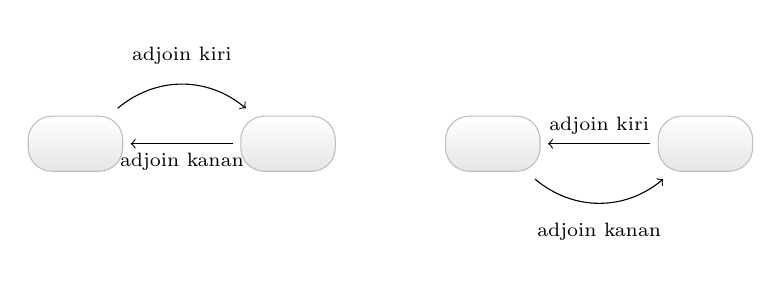
\begin{tikzpicture}[entity/.style={draw, color=black!25, rectangle, rounded corners=3mm, minimum width=12mm, minimum height=7mm, outer sep=1mm, top color=white, bottom color=black!10} ]
		\node[entity] (A) at (0,0) {};
		\node[entity] (B) at (2.7, 0) {};
		\draw (A) edge[->, bend left=40] node[above, inner sep=0.7em]{\scriptsize adjoin kiri} (B);
		\draw (B) edge[->] node[below] {\scriptsize adjoin kanan} (A);

		\node[entity] (C) at (5.3, 0) {};
		\node[entity] (D) at (8, 0) {};
		\draw (C) edge[->, bend right=40] node[below, inner sep=0.7em]{\scriptsize adjoin kanan} (D);
		\draw (D) edge[->] node[above] {\scriptsize adjoin kiri} (C);
	\end{tikzpicture}\end{center}
	Semua isomorfisme adjoin yang terlibat berasal dari Teorema \ref{prop:Hom-tensor-adjunction}.
\end{corollary}
\begin{proof}
	Pembuktian untuk modul kiri dan kanan sama; berikut hanya ditinjau modul kiri ${}_R M$, ${}_S N$. Lemma \ref{prop:forgetful-as-tensor-Hom} bersama Teorema \ref{prop:Hom-tensor-adjunction} menyiratkan
	\begin{align*}
		\Hom\left( {}_R M, {}_{R \to S} \mathcal{F} ({}_S N) \right) & \simeq \Hom\left( {}_R M, \Hom({}_S S, {}_S N) \right) \\
		& \simeq \Hom\left( S \dotimes{R} M, {}_S N \right)
	\end{align*}
	dengan setiap langkah merupakan isomorfisme kanonik. Jadi, diperoleh relasi adjoin $(S \dotimes{R} -, {}_{R \to S} \mathcal{F})$. Demikian pula,
	\begin{align*}
		\Hom\left({}_{R \to S} \mathcal{F} ({}_S N), {}_R M \right) & \simeq \Hom\left( {}_R S \dotimes{S} N, {}_R M \right) \\
		& \simeq \Hom\left( {}_S N, \Hom( {}_R S, {}_R M) \right),
	\end{align*}
	dan setiap langkah merupakan isomorfisme kanonik. Ini membuktikan pernyataan.
\end{proof}

Untuk homomorfisme gelanggang $f: R \to S$ yang diberikan, fungtor-fungtor dalam Korolari \ref{prop:IP-vs-F} juga ditulis sebagai \index[sym1]{P_RS@$P_{R \to S}$}\index[sym1]{I_RS@$I_{R \to S}$} \index{perubahan basis@perubahan basis (base change)}
\begin{gather*}
	P_{R \to S} := - \dotimes{R} S, \quad I_{R \to S} := \Hom(S_R, (-)_R); \\
	{}_{R \to S} P := {}_S S \dotimes{R} -, \quad {}_{R \to S} I := \Hom({}_R S, {}_R (-)).
\end{gather*}
Huruf P mengisyaratkan ``proyeksi'', sedangkan I mengisyaratkan ``induksi''; keduanya jelas merupakan fungtor aditif. Dalam praktik, kita sering memerlukan deskripsi eksplisit dari isomorfisme adjoin di atas. Sebagai contoh, untuk pasangan adjoin $({}_{R \to S} P, {}_{R \to S}\mathcal{F})$, isomorfisme dalam pembuktian, jika dijabarkan dari definisinya, adalah
\begin{equation}\label{eqn:IP-adjunction-explicit-1} \begin{tikzcd}[row sep=small]
	\Hom\left( {}_R M, {}_{R \to S} \mathcal{F} ({}_S N)\right) \arrow[r, "\sim"] & \Hom\left( {}_R M, \Hom({}_S S, {}_S N) \right) \arrow[r, "\sim"] & \Hom\left( S \dotimes{R} M, {}_S N \right) \\
	f \arrow[mapsto, r] & \left[ m \mapsto [s \mapsto s(mf)] \right] \arrow[mapsto, r] & \left[ s \otimes m \mapsto s(mf) \right] ;
\end{tikzcd}\end{equation}
Kasus modul kanan serupa. Ini adalah rumus yang sering digunakan dalam perhitungan dengan hasil kali tensor.

\begin{lemma}\label{prop:IP-transitivity}
	Tinjau homomorfisme gelanggang $\begin{tikzcd} Q \arrow[r, "f"'] \arrow[rr, bend left=25, "gf"] & R \arrow[r, "g"'] & S \end{tikzcd}$. Fungtor pelupa terkait memenuhi persamaan
	\begin{gather*}
		\mathcal{F}_{Q \to R} \circ \mathcal{F}_{R \to S} = \mathcal{F}_{Q \to S}, \\
		{}_{Q \to R} \mathcal{F} \circ {}_{R \to S} \mathcal{F} = {}_{Q \to S} \mathcal{F};
	\end{gather*}
	sedangkan fungtor $P$, $I$ memenuhi isomorfisme
	\[\begin{array}{ll}
		P_{R \to S} \circ P_{Q \to R} \simeq P_{Q \to S}, & I_{R \to S} \circ I_{Q \to R} \simeq  I_{Q \to S}, \\
		{}_{R \to S} P \circ {}_{Q \to R} P \simeq {}_{Q \to S} P, & {}_{R \to S} I \circ {}_{Q \to R} I \simeq {}_{Q \to S} I.
	\end{array}\]
\end{lemma}
\begin{proof}
	Kasus fungtor pelupa $\mathcal{F}$ jelas. Sisanya mengikuti dari Korolari \ref{prop:IP-vs-F} dan sifat komposisi fungtor adjoin (Proposisi \ref{prop:adjunction-composition}); kasus modul kiri dan kanan tentu serupa.
\end{proof}

Sekarang anggap $R$ suatu gelanggang komutatif. Korolari \ref{prop:module-monoidal-cat} menyatakan bahwa $(R\dcate{Mod}, \otimes, \ldots)$ membentuk kategori monoidal. Untuk konsep fungtor monoidal, lihat Definisi \ref{def:monoidal-functor}.
\begin{proposition}
	Bagi homomorfisme $R \to S$ antara gelanggang-gelanggang komutatif, fungtor $P_{R \to S}: R\dcate{Mod} \to S\dcate{Mod}$ mempunyai struktur fungtor monoidal alami.
\end{proposition}
\begin{proof}
	Kita hanya memberikan isomorfisme fungtor berikut, yang diperlukan bagi fungtor monoidal: \[P_{R \to S}(-) \dotimes{S} P_{R \to S}(-) \xrightarrow[\xi]{\sim} P_{R \to S}\left( - \dotimes{R} - \right).\] Ingat bahwa $P_{R \to S}(M) = M \dotimes{R} S$. Untuk $R$-modul $M$, $N$, definisikan $\xi(M,N)$ sebagai komposisi isomorfisme-isomorfisme berikut:
	\[\begin{tikzcd}[row sep=small, column sep=tiny, every cell/.style={scale=0.93, transform shape, inner xsep=1ex, inner ysep=0.85ex}]
		\left( M \dotimes{R} S \right) \dotimes{S} \left( N \dotimes{R} S \right) \arrow[r, "\sim"] & \left( M \dotimes{R} S \right) \dotimes{S} \left( S \dotimes{R} N \right) \arrow[r, "\sim"] & M \dotimes{R} \left( S \dotimes{R} N \right) \arrow[r, "\sim"] & \left( M \dotimes{R} N \right) \dotimes{R} S \\
		(x \otimes s) \otimes (y \otimes t) \arrow[mapsto, r] & (x \otimes s) \otimes (t \otimes y) \arrow[mapsto, r] & (x \otimes st \otimes y) \arrow[mapsto, r] & (x \otimes y) \otimes st
	\end{tikzcd}\]
	Langkah pertama dan terakhir menggunakan kendala komutativitas $\otimes_R$ (Proposisi \ref{prop:tensor-comm}); langkah-langkah di tengah menggunakan kendala asosiativitas dan kendala satuan $S \dotimes{S} S \rightiso S$ (Proposisi \ref{prop:tensor-unit}). Deskripsi pada baris kedua memudahkan pemeriksaan diagram komutatif dalam Definisi \ref{def:monoidal-functor}, sedangkan syarat $P_{R \to S}(R) = S$ merupakan akibat langsung dari kendala satuan.
\end{proof}
 
\section{Modul Terbangkitkan Hingga atas Daerah Ideal Utama}\label{sec:PID-module}
Semua gelanggang dalam bagian ini adalah daerah integral komutatif tak nol dengan satuan. Untuk ideal utama gelanggang $R$, gunakan notasi baku $(a) := Ra$, dengan $a \in R$. Perhatikan bahwa $(a)(b) = (ab)$. Sekarang terapkan Definisi \ref{def:tor-ann} tentang unsur torsi dan bagian torsi pada daerah integral $R$. Semua unsur torsi dalam sebarang $R$-modul $M$ membentuk submodul $M_\text{tor} \subset M$, yang disebut \emph{submodul torsi}; sebab $ax=0$, $by=0$ menyiratkan $ab(x+y)=0$. Untuk ideal utama $(a)$, bagian torsi terkait $M[\mathfrak{a}] \subset M$ cukup ditulis $M[a]$.

\begin{definition}
	Misalkan $M$ suatu $R$-modul. \emph{Hasil bagi bebas torsi}-nya didefinisikan sebagai modul hasil bagi \index[sym1]{$M_\text{tf}$}\index[sym1]{$M_\text{tor}$}
	\[ M_\text{tf} := M/M_\text{tor}. \]
\end{definition}
Perhatikan bahwa setiap homomorfisme modul $\varphi: M \to N$ memenuhi $\varphi(M_\text{tor}) \subset N_\text{tor}$ dan karena itu menginduksi $\varphi_\text{tf}: M_\text{tf} \to N_\text{tf}$. Jelas bahwa hasil bagi bebas torsi $M \mapsto M_\text{tf}$ sebenarnya memberikan suatu fungtor.

\begin{lemma}
	Hasil bagi bebas torsi $M_\text{tf}$ dari setiap $R$-modul $M$ adalah modul bebas torsi. Tarik balik sepanjang homomorfisme hasil bagi $M \to M_\text{tf}$ memberikan isomorfisme natural
	\[ \Hom_R(M_\text{tf}, N) \rightiso \Hom_R(M, N), \quad \text{jika $N$ adalah $R$-modul bebas torsi.} \]
\end{lemma}
Tulis $R\dcate{Mod}_\text{tf}$ untuk subkategori penuh semua $R$-modul bebas torsi. Maka fungtor $M \mapsto M_\text{tf}$ bersama isomorfisme di atas memberikan fungtor adjoin kiri bagi fungtor inklusi $R\dcate{Mod}_\text{tf} \to R\dcate{Mod}$. Inilah sifat universal hasil bagi bebas torsi.

\begin{proof}
	Misalkan $\bar{x} \in M_\text{tf}$ suatu unsur torsi dan pilih prabayang $x \in M$; untuk pernyataan pertama, cukup dibuktikan $x \in M_\text{tor}$. Ambil $r \in R$, $r \neq 0$, dengan $r\bar{x} = 0$. Maka $rx \in M_\text{tor}$; pilih lagi $s \in R$ tak nol sehingga $srx=0$, dan diperoleh $x \in M_\text{tor}$.

	Sekarang misalkan $N$ bebas torsi dan $\varphi \in \Hom_R(M, N)$. Sifat $\varphi(M_\text{tor}) \subset N_\text{tor} = \{0\}$ bersama Proposisi \ref{prop:1st-homomorphism-module} segera memberikan faktorisasi $\varphi = [M \to M_\text{tf} \xrightarrow{\varphi_\text{tf}} N]$.
\end{proof}

\begin{convention}
	Dalam sisa bagian ini, selalu diasumsikan bahwa $R$ adalah daerah ideal utama (lihat Definisi \ref{def:PID}).
\end{convention}

\begin{lemma}\label{prop:PID-free-submodule}
	Misalkan $E$ modul bebas atas $R$. Setiap submodul $M$ dari $E$ adalah bebas, dan $\rank_R(M) \leq \rank_R(E)$. 
\end{lemma}
Untuk basis dan rank $\rank_R(E)$ dari modul bebas $E$, lihat Definisi \ref{def:rank-module}.
\begin{proof}
	Perhatikan bahwa $M$ bebas torsi. Tetapkan basis $X$ dari $E$ dan tinjau himpunan
	\[ \mathcal{P} := \left\{ (Y,Y',b) :
		\begin{array}{l}
			Y' \subset Y: \; X \; \text{memuat kedua himpunan itu} \\
			M_Y := M \cap \sum_{y \in Y} Ry \; \text{adalah modul bebas} \\
			b: Y' \to M \; \text{adalah suatu peta} \\
			\{b(y) : y \in Y'\} \;\text{membentuk basis dari $M_Y$}
		\end{array}
	\right\}. \]
	Berikan $\mathcal{P}$ urutan parsial
	\[ (Y, Y', b) \leq (Y_1, Y'_1, b_1) \iff (Y \subset Y_1) \wedge (Y' \subset Y'_1) \wedge (b_1|_{Y'} = b). \]
	Jelas bahwa $\mathcal{P}$ tidak kosong (ia memuat $Y=Y'=\emptyset$), dan setiap rantainya mempunyai batas atas: ambil gabungan semua $Y' \subset Y$ dalam rantai tersebut, yaitu $\mathcal{Y}' \subset \mathcal{Y}$, lalu rekatkan fungsi-fungsi $b$ menjadi $\mathcal{Y}' \to M$; hasilnya memberikan basis bagi $M_{\mathcal{Y}}$. Lemma Zorn (Teorema \ref{prop:Zorn}) menjamin bahwa $(\mathcal{P}, \leq)$ mempunyai unsur maksimal. Cukup dibuktikan bahwa setiap unsur maksimal $(Y,Y',b)$ memenuhi $Y=X$; dalam hal ini $\rank_R(M) = |Y'| \leq |X| = \rank_R(E)$.

	Andaikan $(Y,Y',b) \in \mathcal{P}$ dan $Y \neq X$. Untuk $x \in X \smallsetminus Y$, definisikan ideal
	\[ \mathfrak{a} := \left\{a \in R : \left( ax + \sum_{y \in Y} Ry \right) \cap M \neq \emptyset \right\}. \]
	\begin{enumerate}
		\item Jika $\mathfrak{a}=\{0\}$, maka $M_{Y \sqcup \{x\}} = M_Y$. Dengan mengambil $Y_1 = Y \sqcup \{x\}$, $Y'_1 = Y'$, dan $b_1 = b$, diperoleh unsur $\mathcal{P}$ yang secara ketat lebih besar daripada $(Y,Y',b)$.
		\item Jika $\mathfrak{a} \neq \{0\}$, pilih unsur tak nol $a \in R$ sehingga $\mathfrak{a} = (a)$, dan pilih $m_x \in M$ dengan
			\[ m_x \in ax + \sum_{y \in Y} Ry. \]
			Jika sebarang unsur $m'$ dari $M_{Y \sqcup \{x\}}$ dikembangkan dalam $E$ terhadap $Y \sqcup \{x\}$, koefisien $x$ harus berada dalam $(a)$. Karena itu terdapat $r \in R$ sehingga $m' - rm_x \in M_Y$. Maka
			\[ M_{Y \sqcup \{x\}} = Rm_x \oplus M_Y, \]
		sehingga dapat diambil $Y_1 := Y \sqcup \{x\}$, $Y'_1 := Y' \sqcup \{x\}$, dan $b_1: Y_1 \to M$ yang memenuhi $b|_{Y'}=b$, $b(x) = m_x$; data ini memberikan unsur $\mathcal{P}$ yang secara ketat lebih besar daripada $(Y,Y',b)$.
	\end{enumerate}
	Dengan demikian, unsur maksimal $(Y,Y',b)$ dari $(\mathcal{P}, \leq)$ harus memenuhi $Y=X$.
\end{proof}
Jika $\rank_R(E) = |X|$ berhingga, keberadaan unsur maksimal dalam $(\mathcal{P}, \leq)$ pada pembuktian di atas jelas dan tidak memerlukan Lemma Zorn. Sebagai penerapan, diperoleh dekomposisi jumlah langsung berikut.

\begin{proposition}\label{prop:decomp-tor-free}
	Misalkan $M$ suatu $R$-modul dan $M_\text{tf}$ dibangkitkan secara berhingga. Maka $M_\text{tf}$ adalah modul bebas, dan terdapat submodul bebas $E \subset M$ ber-rank hingga sehingga $M = M_\text{tor} \oplus E$.
\end{proposition}
\begin{proof}
	Pilih suatu himpunan pembangkit berhingga $X$ dari $R$-modul bebas torsi terbangkitkan hingga $M_\text{tf}$, lalu ambil subhimpunan bebas linear maksimal $Y$ di dalamnya. Untuk setiap $x \in X \smallsetminus Y$, kita mungkin tidak dapat menulis $x$ sebagai kombinasi linear dari $Y$; tetapi karena $Y \sqcup \{x\}$ bergantung linear, selalu terdapat $a_x \in R$, $a_x \neq 0$, sehingga $a_x x \in \sum_{y \in Y} Ry$. Tetapkan $a := \prod_{x \in X \smallsetminus Y} a_x$. Maka homomorfisme
	\begin{align*}
		M_\text{tf} & \longrightarrow \bigoplus_{y \in Y} Ry = R^{\oplus Y} \\
		m & \longmapsto am
	\end{align*}
	bersifat injektif. Lemma \ref{prop:PID-free-submodule} segera menunjukkan bahwa $M_\text{tf}$ adalah modul bebas ber-rank hingga.

	Pilih basis $B$ dari $M_\text{tf}$, dan untuk setiap $\bar{b} \in B$, pilih prabayang $b \in M$. Mudah diperiksa bahwa $E := \sum_{\bar{b} \in B} Rb = \bigoplus_{\bar{b} \in B} Rb$ adalah submodul bebas dari $M$, dan bahwa pembatasan $M \to M_\text{tf}$ memberikan isomorfisme $E \rightiso M_\text{tf}$. Dengan demikian, $M = M_\text{tor} \oplus E$.
\end{proof}

Berdasarkan Proposisi \ref{prop:decomp-tor-free}, sering kali berguna mereduksi kajian modul terbangkitkan hingga atas $R$ ke kasus $M = M_\text{tor}$. Dalam keadaan ini berlaku dekomposisi berikut. Ingat bahwa daerah ideal utama $R$ merupakan daerah faktorisasi tunggal (Teorema \ref{prop:PID-UFD}).

\begin{lemma}\label{prop:PID-primary-decomp}
	Andaikan $R$-modul $M$ memenuhi $\mathrm{ann}(M) \neq \{0\}$. Misalkan unsur $\prod_{i=1}^m p_i^{n_i}$ dari $R$ membangkitkan ideal $\mathrm{ann}(M)$, dengan $p_1, \ldots, p_m$ unsur-unsur tak tereduksi dari $R$ yang saling tidak membagi. Maka $M$ mempunyai dekomposisi jumlah langsung
	\[ M = \bigoplus_{i=1}^m M[p_i^{n_i}]. \]
	Submodul dalam dekomposisi yang bersesuaian dengan $p = p_i$ juga dapat ditulis secara lebih intrinsik sebagai $M[p^\infty] := \bigcup_{n \geq 0} M[p^n]$ dan disebut \emph{bagian $p$-primer} dari $M$. \index[sym1]{$M[p^\infty]$}\index{bagian $p$-primer ($p$-primary part)}
\end{lemma}
\begin{proof}
	Pandang $M$ sebagai modul atas $R/(\prod_{i=1}^m p_i^{n_i})$. Tetapkan $I_i := (p_i^{n_i})$. Faktorisasi tunggal dalam daerah ideal utama menyiratkan $(\prod_i p_i^{n_i}) = \bigcap_i I_i$, dan $I_1, \ldots, I_m$ memenuhi hipotesis Teorema \ref{prop:CRT}; jadi
	\[ R \big/ ( \prod_{i=1}^m p_i^{n_i} ) \rightiso \prod_{i=1}^m R/(p_i^{n_i}). \]
	Lemma \ref{prop:prod-module} memberikan dekomposisi jumlah langsung terkait $M = \bigoplus_{i=1}^m M_i$, dengan setiap $M_i$ sebenarnya suatu modul atas $R/(p_i^{n_i})$. Dari syarat-syaratnya, untuk setiap $N$ berlaku $(\prod_{j \neq i} p_j^{n_j}) + (p_i^N) = R$; dengan mudah diperoleh $M_i = M[p_i^{n_i}] = M[p_i^{\infty}]$.
\end{proof}

Kini semua persiapan selesai untuk membuktikan teorema struktur modul atas daerah ideal utama beserta akibat-akibatnya.
\begin{theorem}[Teorema pembagi elementer]\label{prop:elementary-divisor-sub}\index{teorema pembagi elementer (Theorem of elementary divisors)}
	Misalkan $E$ modul bebas ber-rank $n$ atas $R$ ($n \in \Z_{\geq 0}$) dan $M$ suatu submodulnya. Maka terdapat basis $\{e_1, \ldots, e_n\}$ dari $E$ dan keluarga ideal $\mathfrak{d}_i = (d_i)$, $i=1, \ldots, n$, yang memenuhi
	\begin{itemize}
		\item $\mathfrak{d}_1 \supset \cdots \supset \mathfrak{d}_n$;
		\item definisikan $0 \leq k \leq n$ melalui $\mathfrak{d}_i \neq (0) \iff i \leq k$. Maka unsur-unsur
			\[ d_i e_i, \quad 1 \leq i \leq k \]
		membentuk basis dari $M$.
	\end{itemize}
	Rantai ideal $\mathfrak{d}_1 \supset \mathfrak{d}_2 \supset \cdots \supset \mathfrak{d}_n$ demikian sepenuhnya ditentukan oleh modul $E$ dan $M$, sedangkan ideal-ideal sejatinya sepenuhnya ditentukan oleh kelas isomorfisme $E/M$.
\end{theorem}
\begin{proof}
	Pertama, buktikan keberadaan basis demikian. Untuk setiap $\lambda \in \Hom_R(E, R)$, bayangan $\lambda(M)$ adalah ideal dari $R$. Keluarga ideal $\{ \lambda(M): \lambda \in \Hom_R(E, R) \}$ selalu mempunyai unsur maksimal terhadap inklusi $\subset$; jika tidak, kita dapat mengekstrak rantai ideal naik tak hingga $\mathfrak{a}_1 \subsetneq \mathfrak{a}_2 \subsetneq \cdots$, bertentangan dengan Lemma \ref{prop:ACC-PID}. Pilih unsur maksimal $\lambda_1(M) = \lrangle{d_1} =: \mathfrak{d}_1$. Jika $d_1 = 0$, maka $M=\{0\}$; dalam hal ini, ambil sebarang basis $e_1, \ldots, e_n$.

	Jika $d_1 \neq 0$, pilih $x_1 \in M$, $x_1 \neq 0$, sehingga $\lambda_1(x_1) = d_1$. Kita menyatakan bahwa untuk setiap $\lambda \in \Hom_R(E, R)$ berlaku $\lambda(x_1) \in (d_1)$; ini ekuivalen dengan pernyataan bahwa ideal $(b) := (\lambda(x_1)) + (d_1)$ memenuhi $(b)=(d_1)$. Jika tidak, $(b) \supsetneq (d_1)$, sehingga terdapat $u, v \in R$ dengan
	\[ b = u\lambda(x_1) + v\lambda_1(x_1) = (u\lambda + v\lambda_1)(x_1) \notin (d_1), \]
	bertentangan dengan maksimalitas $\lambda_1(M)$. Karena $\lambda$ sebarang, semua koordinat $x_1$ terhadap sebarang basis $E$ habis dibagi $d_1$; maka terdapat $e_1 \in E$ sehingga $x_1 = d_1 e_1$.

	Menurut Lemma \ref{prop:PID-free-submodule}, $E' := \Ker(\lambda_1)$ juga modul bebas, dan $E' \cap Re_1 = \{0\}$. Dari $\lambda_1(e_1) = 1$, setiap $e \in E$ mempunyai representasi tunggal
	\[ e = \lambda_1(e) e_1 + \underbracket{e - \lambda_1(e)e_1}_{\in E'} \in R e_1 \oplus E', \]
	sehingga $E = R e_1 \oplus E'$. Jika $e \in M$, maka $\lambda_1(e) e_1 \in (d_1) e_1 = R x_1 \subset M$, sehingga
	\[ M = Rx_1 \oplus \underbracket{(M \cap E')}_{:= M'}. \]
	Ulangi prosedur sebelumnya pada $M' \subset E'$ untuk memperoleh $\mathfrak{d}_2 = (d_2) = \lambda_2(M')$, dengan $\lambda_2 \in \Hom_R(E', R)$. Pilih $x_2 \in M'$ sehingga $\lambda_2(x_2) = d_2$. Kita menyatakan bahwa $\mathfrak{d}_1 \supset \mathfrak{d}_2$: homomorfisme $\lambda_2$ dapat diperluas menjadi $\tilde{\lambda}_2: E \to R$ dengan $\tilde{\lambda}_2(e_1)=0$. Di sisi lain, pilih $u,v \in R$ sehingga $(ud_1 + vd_2) = (d_1) + (d_2)$. Bersama definisi $E'$, diperoleh
	\[ ud_1 + vd_2 = (u \lambda_1 + v\tilde{\lambda}_2)(x_1 + x_2) \in (u \lambda_1 + v\tilde{\lambda}_2)(M), \]
	sehingga maksimalitas $\lambda_1(M)$ memberikan $(d_1) + (d_2) = (d_1)$, yakni $\mathfrak{d}_1 \supset \mathfrak{d}_2$. Dengan mengulangi penurunan rank ini, diperoleh semua $e_i$ dan $\mathfrak{d}_i$ yang diperlukan.

	Terakhir, buktikan ketunggalan. Perhatikan bahwa
	\begin{gather*}
		(E/M)_\text{tor} \simeq \bigoplus_{\substack{1 \leq i \leq k \\ \mathfrak{d}_i \neq R}} R/\mathfrak{d}_i, \quad (E/M)_\text{tf} \simeq R^{\oplus (n-k)}.
	\end{gather*}
	Karena $R$ suatu daerah integral, Catatan \ref{rem:IBN} memungkinkan kita membaca $n-k$ dari $(E/M)_\text{tf}$. Jika data tersisa $\mathfrak{d}_i \neq R$ dapat dibaca dari $N := (E/M)_\text{tor}$, maka $|\{i: \mathfrak{d}_i = R \}|$ juga dapat ditentukan dari $\rank_R(M)$. Jadi kita beralih ke kajian $N := \bigoplus_{i=1}^k R/\mathfrak{d}_i$. Untuk menyederhanakan notasi, anggap $\mathfrak{d}_1 \neq R$.

	Lemma \ref{prop:PID-primary-decomp} menyatakan $N$ sebagai $\bigoplus_p N[p^\infty]$, dan dekomposisi ini hanya bergantung pada struktur modul $N$. Untuk setiap unsur tak tereduksi $p$ yang dipilih, mudah dilihat bahwa $(R/\mathfrak{d}_i)[p^\infty] = R/(p^{n_i})$, dengan $n_i$ banyaknya kemunculan $p$ dalam faktorisasi tak tereduksi $d_i$ (lihat pembuktian Lemma \ref{prop:PID-primary-decomp}). Masalahnya tereduksi ke kasus $d_i = p^{n_i}$, dengan $p$ unsur tak tereduksi tetap dan $1 \leq n_1 \leq n_2 \leq \cdots \leq n_h$.
	
	Tulis $pN$ untuk submodul $\{px: x \in N\}$. Maka terdapat isomorfisme
	\[\begin{tikzcd}[row sep=tiny]
		\frac{N}{pN} \arrow[r, "\sim"] & \bigoplus_{1 \leq i \leq h} \frac{R/(p^{n_i})}{pR/(p^{n_i})} \arrow[rd, "\sim"', "\text{Proposisi \ref{prop:2nd-homomorphism-module}}"] & \\
		& & (R/(p))^{\oplus h} \\
		N[p] \arrow[r, "\sim"] & \bigoplus_{1 \leq i \leq h} p^{n_i - 1} \frac{R}{p^{n_i} R} \arrow[ru, "\sim"] & 
	\end{tikzcd}\]
	Dengan menerapkan pengamatan ini pada $p^j N = \bigoplus_i p^j R/(p^{n_i})$, banyaknya suku jumlah langsung yang tak nol, $\nu_j := |\{i: n_i > j\}|$, dapat dibaca dari struktur modul $p^j N$:
	\begin{gather}\label{eqn:PID-decomp-nu_j}
		\dim_{R/(p)} (p^j N)[p] = \nu_j = \dim_{R/(p)} \frac{p^j N}{p^{j+1} N}.
	\end{gather}

	Mengadaptasi metode \S\ref{sec:symmetric-poly}, sajikan data $n_1 \leq \cdots \leq n_h$ sebagai berikut: dari bawah ke atas, letakkan $n_i$ kotak pada baris ke-$i$, seperti dalam diagram berikut (ambil $n_1=n_2=1$, $n_3=2$, ...): \index{diagram Young}
	\ytableausetup{mathmode}
	\begin{equation}\label{eqn:PID-decomp-diagram} \begin{ytableau}
		\none & \none[\nu_0] & \none[\nu_1] & \none[\cdots] & \none \\
		\none[n_h] & & & \none[\cdots] & \\
		\none[\vdots] & \none[\vdots] & \none[\vdots] \\
		\none[n_3] & & \\
		\none[n_2] & \\
		\none[n_1] &
	\end{ytableau}\end{equation}
	Dengan menghitung secara vertikal, mudah dilihat bahwa kolom ke-$j+1$ mempunyai tepat $\nu_j$ kotak. Jadi data $(n_i)_{i \geq 1}$ dan $(\nu_j)_{j \geq 0}$ merupakan dua sisi dari hal yang sama dan saling menentukan. Dengan \eqref{eqn:PID-decomp-nu_j}, $(\nu_j)_j$ dapat dibaca dari struktur $N$, dan kemudian $(n_i)_i$ dapat dipulihkan.
\end{proof}
Setelah basis $E$ dan para pembangkit $M$ diberikan, pembuktian di atas juga dapat dirumuskan sebagai algoritma matriks; hasilnya disebut bentuk normal Smith dari suatu matriks. Lihat \cite[Bab 6 \S 5]{DN00}.

\begin{theorem}\label{prop:elementary-divisor}
	Setiap modul terbangkitkan hingga $N$ atas daerah ideal utama $R$ isomorfik dengan modul berbentuk
	\[ N \simeq \bigoplus_{i=1}^n R/\mathfrak{d}_i, \quad R \neq \mathfrak{d}_1 \supset \cdots \supset \mathfrak{d}_n \]
	dan rantai ideal sejati $\mathfrak{d}_1 \supset \cdots \supset \mathfrak{d}_n$ ditentukan secara tunggal oleh kelas isomorfisme $N$; ideal-ideal ini disebut pembagi elementer dari $N$.
\end{theorem}
\begin{proof}
	Tuliskan $N$ sebagai $E/M$, dengan $E$ suatu modul bebas atas $R$ ber-rank hingga. Terapkan Teorema \ref{prop:elementary-divisor-sub} pada $M \subset E$.
\end{proof}

Karena $\Z$-modul tidak lain adalah grup abelian (Contoh \ref{eg:Z-modules}), kita langsung memperoleh teorema struktur klasik berikut.
\begin{corollary}\label{prop:finite-abelian-structure}
	Setiap grup abelian terbangkitkan hingga $G$ isomorfik dengan grup berbentuk $\bigoplus_{i=1}^n \Z/d_i\Z$, dengan
	\[ d_1, \ldots, d_n \in \Z_{\geq 0} \smallsetminus \{1\}, \quad d_1 \mid  d_2  \mid  \cdots  \mid  d_n \]
	yang ditentukan secara tunggal oleh kelas isomorfisme $G$. Jika $G$ berhingga, maka $d_1, \ldots, d_n$ semuanya tak nol.
\end{corollary}

\begin{remark}\label{rem:primary-elementary-divisor}
	Dalam mempelajari dekomposisi pada Teorema \ref{prop:elementary-divisor}, pendekatan lain adalah mula-mula memakai Proposisi \ref{prop:decomp-tor-free} untuk mereduksi ke kasus $N = N_\text{tor}$. Dalam keadaan ini, kita dapat
	\begin{inparaenum}[(a)]
		\item terlebih dahulu memakai Lemma \ref{prop:PID-primary-decomp} untuk menulis $N$ secara tunggal sebagai jumlah langsung bagian-bagian $p$-primer, lalu menetapkan $p$ dan mereduksi ke kasus $N = N[p^\infty]$,
		\item atau menguraikan setiap suku jumlah langsung $R/\mathfrak{d}_i$ dari $N$ menjadi bagian-bagian primer (perhatikan bahwa $\mathfrak{d}_i \neq \{0\}$); langkah ini tidak lain adalah Teorema Sisa Cina (Teorema \ref{prop:CRT}).
	\end{inparaenum}
	Kedua jalan tentu berujung pada hasil yang sama. Pada akhirnya, diperoleh keluarga invarian yang lebih halus $(p^{v_1}), (p^{v_2}), \ldots$ untuk $N$, dengan $p$ merentang sejumlah hingga unsur prima dan $v_1 \leq v_2 \leq \cdots$. Modul $N$ secara bersesuaian terurai sebagai jumlah langsung modul-modul $R/(p^{v_i})$. Versi ini kadang lebih nyaman daripada Teorema \ref{prop:elementary-divisor}.
\end{remark}

Berikut penerapan sederhana. Grup abelian $(A,+)$ disebut mempunyai \emph{eksponen} $m \in \Z_{\geq 1}$ jika $mA=\{0\}$; Proposisi \ref{prop:ord-power} menyatakan bahwa setiap grup abelian berhingga mempunyai eksponen. Bagi grup bereksponen $m$, definisikan grup dualnya sebagai $A^\vee := \Hom(A, \frac{1}{m}\Z/\Z)$, dengan penjumlahan $(f_1 + f_2)(\cdot) = f_1(\cdot) + f_2(\cdot)$; grup ini juga bereksponen $m$. Dalam definisi ini, $\frac{1}{m}\Z/\Z$ jelas dapat diganti dengan $\Z/m\Z$; keuntungan pilihan pertama ialah bahwa ia sama dengan $(\Q/\Z)[m] \subset \Q/\Z$. Dengan demikian, $\Hom(A, \frac{1}{m}\Z/\Z) = \Hom(A, \Q/\Z)$ (periksalah), sehingga definisi $A^\vee := \Hom(A, \Q/\Z)$ mencakup semua eksponen sekaligus. \index{grup!eksponen (exponent)}

Sebagai contoh, ambil $A := \Z/n\Z$. Terdapat isomorfisme grup $\Z/n\Z \rightiso A^\vee$ yang memetakan $a + n\Z \in A$ ke unsur $\left[ b+n\Z \mapsto \frac{ab}{n} + \Z \in \Q/\Z \right]$ dari $A^\vee$. Verifikasinya langsung dan diserahkan kepada pembaca.

Semua grup abelian yang mempunyai eksponen membentuk kategori $\cate{Ab}_e$. Jika $\varphi: A \to B$ homomorfisme dalam $\cate{Ab}_e$, secara alami terdapat homomorfisme $\varphi^\vee: B^\vee \to A^\vee$ yang ``menarik balik'' $f$ menjadi $f \circ \varphi$. Jelas bahwa $(\varphi \psi)^\vee = \psi^\vee \varphi^\vee$, sehingga $A \mapsto A^\vee$ memberikan fungtor aditif $D: \cate{Ab}_e \to \cate{Ab}_e^{\text{op}}$. Dalam $\cate{Ab}_e$ terdapat isomorfisme natural
\[\begin{tikzcd}[row sep=tiny]
	(A \times B)^\vee \arrow[r, "\sim"] & A^\vee \times B^\vee &  \\
	f \arrow[phantom, u, "\in" description, sloped] \arrow[mapsto, r] & (f|_{A \times 0}, f|_{0 \times B}) \arrow[phantom, u, "\in" description, sloped] & \left( A, B \in \Obj(\cate{Ab}_e) \right) \\
	\left[ (a,b) \mapsto f_1(a) + f_2(b) \right] & (f_1, f_2) \arrow[mapsto, l] &
\end{tikzcd}\]
Jadi $(f_1, f_2)$ dapat diidentifikasi dengan unsur $(A \times B)^\vee$. Ini juga merupakan akibat formal bahwa fungtor $D$ mempertahankan biproduk (Proposisi \ref{prop:biproduct-preservation}). Selain itu, terdapat homomorfisme ``evaluasi'' natural
\begin{equation}\label{eqn:ab-group-duality} \begin{aligned}
	\iota_A: A & \longrightarrow A^{\vee\vee} = D^\text{op} D(A) \\
	a & \longmapsto \left[ A^\vee \ni f \mapsto f(a) \right].
\end{aligned}\end{equation}
Sebagai latihan sederhana, periksa bahwa untuk setiap $A \xrightarrow{\varphi} B$ berlaku $\varphi^{\vee\vee} \circ \iota_A = \iota_B \circ \varphi$. Dalam bahasa teori kategori di atas, $\iota := (\iota_A)_A$ memberikan morfisme antar-fungtor
$\begin{tikzcd}
	\cate{Ab}_e \arrow[bend left=35, r, "\identity", ""' name=U] \arrow[bend right=35, r, "{D^\text{op} D}"', "" name=D] & \arrow[Rightarrow, to path=(U) -- (D) \tikztonodes, "\iota"] \cate{Ab}_e
\end{tikzcd}$.
Kini Contoh \ref{eg:vectf-duality} mempunyai analog berikut.
\begin{corollary}[Dualitas grup abelian berhingga]\label{prop:finite-duality}
	Misalkan $A$ suatu grup abelian berhingga. Maka $\iota_A: A \rightiso A^{\vee\vee}$.
\end{corollary}
\begin{proof}
	Tulis $\Psi_{A,B}$ untuk isomorfisme natural di atas, $(A \times B)^{\vee\vee} \rightiso (A^\vee \times B^\vee)^\vee \rightiso A^{\vee\vee} \times B^{\vee\vee}$. Seperti yang diharapkan, dengan menjabarkan definisinya terlihat bahwa diagram berikut komutatif:
	\[\begin{tikzcd}[row sep=tiny]
		& (A \times B)^{\vee\vee} \arrow[dd, "\simeq"', "\Psi_{A,B}"] & \lambda \arrow[phantom, l, "\ni" description, sloped] \arrow[mapsto, dd] \\
		A \times B \arrow[ru, "{\iota_{A \times B}}"] \arrow[rd, "\iota_A \times \iota_B"'] & \\
		& A^{\vee\vee} \times B^{\vee\vee} & \arrow[phantom, l, "\ni" description, sloped] \left( f_A \mapsto \lambda((f_A, 0)), \; f_B \mapsto \lambda((0, f_B)) \right)
	\end{tikzcd}\]
	Menurut Korolari \ref{prop:finite-abelian-structure}, masalah tereduksi ke kasus $A = \Z/n\Z$. Deskripsi $(\Z/n\Z)^\vee$ di atas langsung menunjukkan bahwa $\iota_{\Z/n\Z}$ adalah isomorfisme.
\end{proof}
Jadi $\iota: \identity \to D^\text{op} D$ merupakan isomorfisme antar-fungtor, sedangkan $D, D^\text{op}$ adalah ekuivalensi kategori aditif. Berikut adalah akibat formal dari ``dualitas'' ini.

\begin{corollary}\label{prop:finite-duality-2}
	Misalkan $H$ subgrup dari grup abelian berhingga $A$. Peta $f \mapsto f|_H$ memberikan homomorfisme ``restriksi'' $r_H: A^\vee \to H^\vee$; tulis kernelnya sebagai $H^\perp$. Maka
	\begin{compactenum}[(i)]
		\item $r_H: A^\vee/H^\perp \rightiso H^\vee$;
		\item $H^\perp = (A/H)^\vee \hookrightarrow A^\vee$;
		\item sebagai subgrup dari $A^{\vee\vee}$, berlaku $H^{\vee\vee} = H^{\perp\perp}$, dan $\iota_A|_H: H \rightiso H^{\perp\perp}$.
	\end{compactenum}
\end{corollary}
\begin{proof}
	Karena $D$ memberikan ekuivalensi kategori aditif, ia mengubah $A/H = \Coker\left[H \hookrightarrow A\right]$ menjadi $\Ker(r_H) = H^\perp$, serta mengubah $H = \Ker[A \to A/H]$ menjadi $\Coker\left[ (A/H)^\vee \to A^\vee \right] = \Coker\left[ H^\perp \hookrightarrow A^\vee \right] = A^\vee/H^\perp$. Ini membuktikan (i) dan (ii).
	
	Selanjutnya tinjau (iii). Pandang $H \hookrightarrow A$ sebagai kernel dari $A \to A/H$. Karena $D^\text{op} D$ mempertahankan kernel, homomorfisme natural terinduksi $H^{\vee\vee} \to A^{\vee\vee}$ dapat diidentifikasi dengan $\Ker\left[ A^{\vee\vee} \to (A/H)^{\vee\vee}\right]$. Namun $A^{\vee\vee} \to (A/H)^{\vee\vee} \simeq (H^\perp)^\vee$ tidak lain adalah $r_{H^\perp}$, yang kernelnya tepat $H^{\perp\perp}$. Karena pembatasan $\iota_A$ pada $H$ adalah $\iota_H: H \rightiso H^{\vee\vee}$ (akibat fungtorialitas $\iota$), (iii) terbukti.
\end{proof}
Pembaca tentu mengenal sifat serupa untuk ruang vektor berdimensi hingga dan ruang dualnya.
 
\section{Pengantar Barisan Eksak}\label{sec:exactseq-module}
Tetapkan gelanggang $R$. Berikut hanya ditinjau modul kiri atas $R$; kasus modul kanan atas $R$ (yakni modul kiri atas $R^\text{op}$) sepenuhnya sama. Kasus bimodul $(R,S)$ juga dapat ditangani dengan cara serupa.

Kategori modul $R\dcate{Mod}$ adalah model bagi apa yang disebut kategori abelian. Rinciannya ditunda hingga bab aljabar homologis. Secara kasar, ini berarti bahwa
\begin{itemize}
	\item $R\dcate{Mod}$ adalah kategori aditif (Korolari \ref{prop:Mod-cat-additive}); khususnya, terdapat biproduk dalam $R\dcate{Mod}$, dan himpunan homomorfisme $\Hom_R(M, N)$ mempunyai struktur grup aditif alami;
	\item setiap morfisme $f: M \to N$ dalam $R\dcate{Mod}$ mempunyai kernel $\Ker(f) \hookrightarrow M$ dan kokernel $N \twoheadrightarrow \Coker(f)$, yang masing-masing merupakan kasus khusus ekualiser dan koekualiser dalam teori kategori (lihat Teorema \ref{prop:module-cat-completeness});
	\item berdasarkan butir sebelumnya, morfisme natural $M/\Ker(f) \to \Ker\left[ N \to \Coker(f) \right]$ adalah isomorfisme; ini langsung dari definisi.
\end{itemize}
Dari sifat-sifat di atas dapat dibangun teori umum aljabar homologis, sebagaimana dirintis oleh Grothendieck dalam \cite{Gr57}. Namun, semua hasil dalam bagian ini dapat diperiksa langsung dari sudut pandang modul.

\begin{definition}\index{kompleks@kompleks (complex)}\index{barisan eksak}
	Sebuah \emph{kompleks} $R$-modul adalah suatu barisan $R$-modul beserta homomorfisme berturutan di antaranya, berbentuk
	\[ \cdots \to W \to X \to Y \to Z \to \cdots, \]
	yang dapat memanjang tak hingga atau mempunyai ujung pada satu atau kedua sisi. Kita mensyaratkan bahwa setiap dua homomorfisme yang tersambung ujung-ke-pangkal
	\[ X \to Y \to Z, \]
	berkomposisi menjadi peta nol $X \xrightarrow{0} Z$, atau secara ekuivalen $\Image[X \to Y] \subset \Ker[Y \to Z]$. \emph{Grup homologi} kompleks pada $Y$ didefinisikan sebagai $R$-modul \index{homologi@homologi (homology)}
	\[ \Ker[Y \to Z] \big/ \Image[X \to Y]. \]
	Jika $\Ker[Y \to Z] = \Image[X \to Y]$, kompleks disebut \emph{eksak} pada suku $Y$. Kompleks yang eksak di setiap suku disebut \emph{barisan eksak}.
\end{definition}

Biasanya suku-suku kompleks diberi indeks bilangan bulat dan ditulis $[ \cdots \to  M_i \xrightarrow{d_i} M_{i-1} \to \cdots]$ atau $(M_\bullet, d_\bullet)$. Syarat kompleks lalu menjadi, untuk setiap suku $M_i$ yang bukan ujung,
\[ d_i d_{i+1} = 0, \]
sedangkan grup homologi pada suku ke-$i$ ditulis
\[ \Hm_i(M_\bullet) := \frac{\Ker[d_i: M_i \to M_{i-1}]}{\Image[d_{i+1}: M_{i+1} \to M_i ]}. \]
Keeksakan menjadi syarat $\Hm_i(M_\bullet) = 0$.

Kompleks tanpa ujung $M_\bullet$ dapat terbatas atas ($k \gg 0 \implies M_k = 0$), terbatas bawah ($k \gg 0 \implies M_{-k}=0$), atau terbatas ($|k| \gg 0 \implies M_k = 0$). Suku-suku nol berlebih dapat dihilangkan tanpa memengaruhi keeksakan; misalnya, kompleks terbatas selalu dapat ditulis dalam bentuk $0 \to M_n \to \cdots \to M_1 \to 0$.

Jika kompleks diindeks dengan superskrip $(M^\bullet, d^\bullet)$ dan disyaratkan $d^i: M^i \to M^{i+1}$, teorinya sepenuhnya serupa. Karena indeks berada di atas, \index[sym1]{Hi@$\Hm^i$, $\Hm_i$}
\[ \Hm^i(M^\bullet) := \frac{\Ker[d^i: M^i \to M^{i+1}]}{\Image[d^{i-1}: M^{i-1} \to M^i]}. \]
disebut \emph{grup kohomologi} pada $i$. Kedua konvensi indeks dihubungkan dengan menetapkan $M^i := M_{-i}$ dan mengambil $d^i: M^i \to M^{i+1}$ sebagai $d_{-i}$. \index{kohomologi@kohomologi (cohomology)}

Sesekali kita juga menangani kompleks siklik, yang berarti indeks dalam definisi diambil dari $i \in \Z/n\Z$. Homomorfisme $d_i$ sering cukup ditulis $d$.
\begin{definition}
	Untuk dua kompleks $M_\bullet$, $N_\bullet$ dengan konvensi indeks yang sama, suatu morfisme di antaranya adalah keluarga homomorfisme $\phi = (\phi_i: M_i \to N_i)_i$ yang membuat diagram berikut komutatif untuk setiap $i$:
	\[ \begin{tikzcd}
	M_i \arrow[r, "d_i"] \arrow[d, "{\phi_i}"'] & M_{i-1} \arrow[d, "{\phi_{i-1}}"] \\
	N_i \arrow[r, "d_i"'] & N_{i-1}.
	\end{tikzcd}\]
	Dengan demikian terdapat konsep isomorfisme kompleks, dan kompleks-kompleks $R$-modul dengan ujung tertentu (atau tak terbatas) membentuk suatu kategori. Morfisme $\phi$ menginduksi homomorfisme yang jelas pada tingkat homologi, $\Hm_i(\phi): \Hm_i(M_\bullet) \to \Hm_i(N_\bullet)$.
\end{definition}
Homologi membentuk keluarga fungtor aditif $(\Hm_i)_{a<i<b}$ dari kategori kompleks ke $\cate{Ab}$. Selain itu, keluarga kompleks $(M_{\bullet,i})_{i \in I}$ dapat dibangun suku demi suku menjadi
\begin{compactitem}
	\item produk $\prod_i M_{\bullet,i}$,
	\item jumlah langsung $\bigoplus_i M_{\bullet,i}$, atau lebih umum,
	\item limit $\varprojlim_i M_{\bullet,i}$ atau $\varinjlim_i M_{\bullet,i}$.
\end{compactitem}
Dalam kasus limit, $I$ harus merupakan kategori kecil. Untuk setiap morfisme $i \to j$ dalam $I$, perlu diberikan apa yang disebut homomorfisme transisi $M_{\bullet,j} \to M_{\bullet,i}$ (untuk $\varprojlim$) atau $M_{\bullet,i} \to M_{\bullet,j}$ (untuk $\varinjlim$), yang kompatibel dengan komposisi morfisme dalam $I$; di sini semua homomorfisme tentu berarti homomorfisme kompleks. Fungtorialitas menunjukkan bahwa $\forall i, \; g_i f_i = 0 \implies (\prod_i g_i) (\prod_i f_i)=0$, dan seterusnya; jadi konstruksi-konstruksi ini tetap menghasilkan kompleks.

\begin{lemma}\label{prop:mod-prod-exactness}
	Produk (atau jumlah langsung) suatu keluarga kompleks $(M_{\bullet,i})_i$ eksak jika dan hanya jika setiap $M_{\bullet,i}$ eksak. $\varinjlim$ terarah ke atas dari barisan-barisan eksak (lihat Catatan \ref{rem:filtrant-mod-limit}) tetap eksak.
\end{lemma}
\begin{proof}
	Untuk menangani keeksakan, cukup ditinjau kompleks tiga suku $L_i \xrightarrow{f_i} M_i \xrightarrow{g_i} N_i$. Jelas bahwa $\Image(\prod_i f_i) = \prod_i \Image(f_i)$ dan $\Ker(\prod_i g_i) = \prod_i \Ker(g_i)$; hal yang sama berlaku dengan $\bigoplus_i$ menggantikan $\prod_i$, sehingga pernyataan pertama jelas. Dalam kasus $\varinjlim$ terarah ke atas, harus dibuktikan $\Ker(\varinjlim_i g_i) \subset \Image(\varinjlim_i f_i)$. Ini merupakan penerapan langsung konstruksi dalam Catatan \ref{rem:filtrant-mod-limit} dan diserahkan sebagai latihan.
\end{proof}

Berikutnya, kita tinjau beberapa jenis barisan eksak yang paling sederhana. Ingat bahwa satu-satunya homomorfisme dari atau ke modul nol adalah homomorfisme nol.
\begin{itemize}
	\item Barisan $0 \to M \to 0$ eksak jika dan hanya jika $M = \{0\}$;
	\item barisan $0 \to M' \to M$ eksak jika dan hanya jika $M' \to M$ injektif: keeksakan ekuivalen dengan $\Ker[M' \to M] = \Image[0 \to M'] = 0$;
	\item barisan $M \to M'' \to 0$ eksak jika dan hanya jika $M \to M''$ surjektif: keeksakan ekuivalen dengan $\Image[M \to M''] = \Ker[M'' \to 0] = M''$;
	\item barisan $0 \to M' \to M \to 0$ eksak jika dan hanya jika $M \to M'$ adalah isomorfisme; ini merupakan akibat dua pernyataan sebelumnya.
\end{itemize}

\begin{definition}\index{barisan eksak!pendek}
	\emph{Barisan eksak pendek} adalah barisan eksak berbentuk $0 \to M' \xrightarrow{f} M \xrightarrow{g} M'' \to 0$.
\end{definition}
Menurut contoh di atas, $M' \hookrightarrow M$ dalam barisan eksak pendek dapat dipandang sebagai penyertaan submodul, sedangkan $M \to M''$ surjektif. Keeksakan pada suku tengah $M$ ekuivalen dengan $\Ker[M \xrightarrow{g} M''] = M'$. Jadi, menurut Proposisi \ref{prop:quotient-image-module}, hingga isomorfisme kompleks, barisan eksak pendek tidak lain adalah deskripsi konstruksi modul hasil bagi $M'' = M/M'$. Barisan eksak pendek modul dapat dianalogikan dengan ekstensi grup yang dibahas dalam \S\ref{sec:group-extensions}, tetapi kasus modul lebih sederhana. Sejalan dengan pembelahan ekstensi grup, barisan eksak pendek modul juga mempunyai konsep pembelahan yang terkait dengan dekomposisi biproduk modul (lihat Definisi \ref{def:biproduct}). 

\begin{proposition}\label{prop:split-ses-mod}
	Misalkan $0 \to M' \xrightarrow{f} M \xrightarrow{g} M'' \to 0$ suatu barisan eksak pendek dalam kategori $R\dcate{Mod}$. Pernyataan berikut ekuivalen.
	\begin{enumerate}[(i)]
		\item Terdapat $s: M'' \to M$ sehingga $gs = \identity_{M''}$.
		\item Terdapat $r: M \to M'$ sehingga $rf = \identity_{M'}$.
		\item Terdapat diagram $\begin{tikzcd} M' \arrow[yshift=-0.7ex, r, "f"'] & M \arrow[yshift=0.7ex, l, "r"'] \arrow[yshift=-0.7ex, r, "g"'] & M'' \arrow[yshift=0.7ex, l, "s"'] \end{tikzcd}$ yang membuat $M$ menjadi biproduk $M' \oplus M''$.
		\item Peta $g_*: \Hom(X, M) \to \Hom(X, M'')$ surjektif untuk setiap $R$-modul $X$.
		\item Peta $f^*: \Hom(M, X) \to \Hom(M', X)$ surjektif untuk setiap $R$-modul $X$.
	\end{enumerate}
	Jika salah satu syarat di atas dipenuhi, barisan eksak pendek $0 \to M' \to M \to M'' \to 0$ disebut \emph{terbelah}.
\end{proposition}
Ingat bahwa $g_*(\varphi) = g\varphi$ dan $f^*(\psi) = \psi f$. Berdasarkan pertimbangan topologis, untuk $f: M' \to M$ dan $g: M \to M''$ yang diberikan, jika $gs = \identity$, $s$ disebut suatu \emph{seksi} dari $g$; jika $rf = \identity$, $r$ disebut suatu \emph{retraksi} dari $f$. Keberadaan seksi dan retraksi masing-masing menyiratkan bahwa $g$ surjektif dan $f$ injektif.
\begin{proof}
	Pertama buktikan (i) $\implies$ (iii). Jika $gs = \identity_{M''}$, maka $g( \identity_M - sg) = g - gsg = 0$, sehingga terdapat $r: M \to M'$ dan faktorisasi $(\identity_M - sg) = fr $. Dengan mengomposisikan $f$ di sebelah kanan, diperoleh $frf = f-sgf = f$. Karena $f$ injektif, $rf=\identity_{M'}$. Dengan demikian, diperoleh sifat-sifat pendefinisi biproduk
	\[ rf = \identity_{M'}, \quad gs = \identity_{M''}, \quad fr + sg  = \identity_M. \]
	Demikian pula, mulai dari $rf = \identity_{M'}$, diperoleh $s: M'' \to M$ sehingga $(\identity_M - fr) = sg$, yang membuktikan (ii) $\implies$ (iii). Implikasi (iii) $\implies$ (i), (ii) jelas.
	
	Dari $g_* s_* = (gs)_*$ dan $f^* r^* = (rf)^*$, diperoleh (i) $\implies$ (iv) dan (ii) $\implies$ (v). Sebaliknya, dengan mengambil $X = M''$ dalam (iv), diperoleh $s \in \Hom_R(M'', M)$ sehingga $g_*(s) = gs = \identity_{M''}$; jadi (iv) $\implies$ (i). Demikian pula, mengambil $X = M'$ menunjukkan (v) $\implies$ (ii).
\end{proof}

Sekarang kita perkenalkan alat dasar untuk mempelajari barisan eksak, yang lazim disebut \emph{Lemma Ular}. Tinjau diagram komutatif berikut:
\[\begin{tikzcd}
	& \Ker' \arrow[r] \arrow[d] & \Ker \arrow[r] \arrow[d] & \Ker'' \arrow[d] & \\
	& X' \arrow[d] \arrow[r]  & X \arrow[d] \arrow[r]  & X'' \arrow[r] \arrow[d, ""{coordinate, name=Z}] & 0  \\
	0 \arrow[r] & Y' \arrow[r] \arrow[d] & Y \arrow[r] \arrow[d] & Y'' \arrow[d] & \\
	& \Coker' \arrow[uuurr, "\delta" description, crossing over, dashed, leftarrow, rounded corners, to path= {-- ([xshift=-2ex]\tikztostart.west) |- (Z) [near end]\tikztonodes -| ([xshift=2ex]\tikztotarget.east) -- (\tikztotarget) } ] \arrow[r] & \Coker \arrow[r] & \Coker'' &
\end{tikzcd}\]
di mana
\begin{itemize}
	\item $X' \to X \to X'' \to 0$ dan $0 \to Y' \to Y \to Y''$ keduanya barisan eksak,
	\item $\Ker' := \Ker[X' \to Y'] \hookrightarrow X'$, dan $\Ker$, $\Ker''$ didefinisikan serupa,
	\item $Y' \twoheadrightarrow \Coker' := \Coker[X' \to Y']$, dan $\Coker$, $\Coker''$ didefinisikan serupa; jadi setiap kolom vertikal dalam diagram eksak,
	\item homomorfisme $X' \to X$, $Y' \to Y$, dan seterusnya secara alami menginduksi homomorfisme $\Ker' \to \Ker$, $\Coker' \to \Coker$, dan seterusnya.
\end{itemize}
Dari konstruksinya, bagian garis penuh jelas membentuk diagram komutatif. Konstruksi \emph{homomorfisme penghubung} $\delta: \Ker'' \dashrightarrow \Coker'$ masih perlu dijelaskan; kita bagi menjadi tiga langkah:
\begin{compactenum}[(i)]
	\item Untuk $x'' \in \Ker''$ yang diberikan, keeksakan $X \to X'' \to 0$ memungkinkan kita memilih $x \in X$ dengan $x \mapsto x''$.
	\item Misalkan $y \in Y$ bayangan $x$ di bawah $X \to Y$. Kekomutatifan diagram menunjukkan $y \in \Ker[Y \to Y'']$.
	\item Karena $Y' \to Y \to Y''$ eksak, terdapat tepat satu $y' \in Y'$ dengan $y' \mapsto y$; kemudian petakan $y' \mapsto \bar{y}' \in \Coker'$.
\end{compactenum}
Dengan menggunakan kekomutatifan dan keeksakan diagram, dua pilihan $x$ pada langkah pertama berbeda paling banyak sebesar bayangan $X' \to X$. Karena itu, nilai $y$ pada langkah kedua berbeda paling banyak sebesar bayangan $X' \to Y' \hookrightarrow Y$, dan $\bar{y}'$ tidak bergantung pada pilihan $x$. Jadi homomorfisme penghubung $\delta(x'') = \bar{y}'$ terdefinisi dengan baik.

\begin{proposition}\label{prop:snake-lemma-mod}\index{Lemma Ular (Snake Lemma)}
	Barisan $\Ker' \to \Ker \to \Ker'' \xrightarrow{\delta} \Coker' \to \Coker \to \Coker''$ eksak.
\end{proposition}
\begin{proof}
	Kita hanya memeriksa suku $\Ker''$ dan $\Coker'$; yang lain mudah. Andaikan dalam konstruksi di atas $x'' \mapsto \bar{y}' = 0$. Dengan menelusuri konstruksi, ini ekuivalen dengan keberadaan $x' \in X'$ sehingga $x - (x'\;\text{yang dipetakan}) \in \Ker$. Karena $X' \to X \to X''$ eksak, pernyataan terakhir ekuivalen dengan $x'' \in \Image[\Ker \to \Ker'']$. Jadi barisan eksak pada $\Ker''$.

	Sekarang tinjau $y' \in Y'$ dan bayangannya $\bar{y}' \in \Coker'$. Syarat $\bar{y}' \mapsto 0 \in \Coker$ ekuivalen dengan $\exists x_0 \in X$ yang dipetakan ke bayangan $y' \in Y'$ dalam $Y$. Bayangan $x_0$ di bawah $X \to X'' \to Y''$ otomatis nol, sehingga $x_0 \mapsto x'' \in \Ker''$. Dengan mengingat konstruksi homomorfisme penghubung $\delta$, diperoleh bahwa $\bar{y}' \mapsto 0$ ekuivalen dengan adanya $x'' \in \Ker''$ sehingga $\delta(x'') = \bar{y}'$.
\end{proof}
Teknik pembuktian ini adalah contoh khas ``penelusuran diagram''; salah satu cirinya ialah mencobanya sendiri sering lebih cepat daripada membacanya. Berikut contoh berguna lain, yang disebut \emph{Lemma Lima}. Atas alasan tersebut, pembuktiannya diserahkan kepada pembaca.

\begin{proposition}\label{prop:5-lemma-mod}
	Tinjau diagram komutatif $R$-modul
	\[\begin{tikzcd}
		X_1 \arrow[r] \arrow[d, "f_1"] & X_2 \arrow[r] \arrow[d, "f_2"] & X_3 \arrow[r] \arrow[d, "f_3"] & X_4 \arrow[r] \arrow[d, "f_4"] & X_5 \arrow[d, "f_5"] \\
		Y_1 \arrow[r] & Y_2 \arrow[r] & Y_3 \arrow[r] & Y_4 \arrow[r] & Y_5
	\end{tikzcd}\]
	dan andaikan kedua baris horizontal eksak.
	\begin{enumerate}
		\item Jika $f_1$ surjektif dan $f_2, f_4$ injektif, maka $f_3$ injektif;
		\item jika $f_5$ injektif dan $f_2, f_4$ surjektif, maka $f_3$ surjektif;
		\item khususnya, jika $f_1$ surjektif, $f_5$ injektif, dan $f_2, f_4$ isomorfisme, maka $f_3$ isomorfisme.
	\end{enumerate}
\end{proposition}

Untuk memahami definisi berikutnya, perhatikan bahwa jika $0 \to X' \to X \to X''$ suatu kompleks, Proposisi \ref{prop:1st-homomorphism-module} menunjukkan bahwa $X' \to X$ difaktorkan melalui $X' \to \Ker[X \to X'']$. Menurut pembahasan sebelumnya, kompleks itu eksak jika dan hanya jika $X' \rightiso \Ker[X \to X'']$. Demikian pula, kompleks $X' \to X \to X'' \to 0$ menginduksi morfisme $\Coker[X' \to X] \to X''$, dan keeksakan ekuivalen dengan $\Coker[X' \to X] \rightiso X''$.

\begin{definition}
	Misalkan $R$, $S$ gelanggang dan $F: R\dcate{Mod} \to S\dcate{Mod}$ suatu fungtor aditif.
	\begin{itemize}
		\item Jika untuk setiap barisan eksak $0 \to X' \to X \to X''$ dalam $R\dcate{Mod}$, bayangannya $0 \to FX' \to FX \to FX''$ juga eksak, maka $F$ disebut fungtor \emph{eksak kiri};
		\item jika untuk setiap barisan eksak $X' \to X \to X'' \to 0$ dalam $R\dcate{Mod}$, bayangannya $FX' \to FX \to FX'' \to 0$ juga eksak, maka $F$ disebut fungtor \emph{eksak kanan};
		\item fungtor yang eksak kiri dan kanan disebut \emph{fungtor eksak}.\index{fungtor!eksak (exact)}
	\end{itemize}
\end{definition}

Keeksakan kiri/kanan fungtor dipertahankan oleh komposisi. Karena fungtor aditif $F$ mempertahankan morfisme nol, untuk $(M_\bullet, d_\bullet)$ yang diberikan, bayangannya $(FM_\bullet, F(d_\bullet))$ tetap merupakan kompleks. Definisi fungtor eksak kiri ekuivalen dengan mempertahankan kernel morfisme. Memang, menurut pembahasan sebelum definisi, $F$ eksak kiri jika dan hanya jika, apabila $0 \to X' \to X \to X''$ eksak, morfisme komposit natural
\[\begin{tikzcd}
	F(\Ker[X \to X'']) \arrow[rr, bend left=15] & FX' \arrow[l, "\sim"'] \arrow[r] & \Ker[FX \to FX'']
\end{tikzcd}\]
adalah isomorfisme, yakni $F$ mempertahankan kernel. Demikian pula, keeksakan kanan ekuivalen dengan $F$ mempertahankan kokernel. Perhatikan pula bahwa dalam kategori modul selalu berlaku $\Image[X \to Y] = \Ker[Y \to \Coker(X \to Y)]$; jadi fungtor eksak juga mempertahankan bayangan morfisme.

Perhatikan bahwa $(M_\bullet, d_\bullet)$ dapat diuraikan menjadi gabungan kompleks-kompleks
\begin{gather*}
	\mathfrak{C}_i: \quad 0 \to N_i \hookrightarrow M_i \xrightarrow{d_i} N_{i-1} \to 0, \qquad N_i := \Ker(d_i)
\end{gather*}
Sebaliknya, dari suatu rangkaian $(\mathfrak{C}_i)_i$ yang diberikan, kita dapat menyambungkannya kembali menjadi kompleks $(M_\bullet, d_\bullet)$; dan $(M_\bullet, d_\bullet)$ eksak jika dan hanya jika setiap $\mathfrak{C}_i$ eksak. Jadi untuk memeriksa keeksakan $F$, cukup meninjau barisan eksak pendek.

\begin{proposition}
	Untuk fungtor aditif $F: R\dcate{Mod} \to S\dcate{Mod}$, pernyataan berikut ekuivalen: 
	\begin{compactitem}
		\item $F$ eksak,
		\item $F$ mempertahankan semua barisan eksak pendek,
		\item $F$ mempertahankan semua barisan eksak.
	\end{compactitem}
	Jika $F$ eksak, maka untuk setiap kompleks $(M_\bullet, d_\bullet)$ dan setiap $i$ terdapat isomorfisme natural $\Hm_i(FM_\bullet) \rightiso F(\Hm_i(M_\bullet))$.
\end{proposition}
\begin{proof}
	Bagian pertama telah dijelaskan. Untuk bagian kedua, perhatikan bahwa fungtor eksak mempertahankan kernel, bayangan, dan kokernel morfisme hingga isomorfisme; karena itu, ia menginduksi isomorfisme
	\[ \frac{\Ker(F(d_i))}{\Image(F(d_{i+1}))} \rightiso \frac{F(\Ker(d_i))}{F(\Image(d_{i+1}))}. \]
	Pernyataan terbukti.
\end{proof}

Ingat kembali konsep fungtor yang mempertahankan limit (Definisi \ref{def:preservation-limit}). Dalam bagian ini, semuanya dipertimbangkan dalam kategori-$\cate{Ab}$.
\begin{proposition}
	Fungtor aditif $F: R\dcate{Mod} \to S\dcate{Mod}$ eksak kiri jika dan hanya jika mempertahankan semua $\varprojlim$ berhingga, dan eksak kanan jika dan hanya jika mempertahankan semua $\varinjlim$ berhingga.
\end{proposition}
\begin{proof}
	Proposisi \ref{prop:biproduct-preservation} menyatakan bahwa fungtor aditif mempertahankan biproduk, sehingga mempertahankan semua produk dan koproduk berhingga. Karena $F$ eksak kiri (atau kanan) ekuivalen dengan mempertahankan kernel (atau kokernel), dan dalam kategori-$\cate{Ab}$ sifat terakhir ekuivalen dengan $F$ mempertahankan ekualiser (atau koekualiser), hasilnya mengikuti dari Catatan \ref{rem:preservation-limit}.
\end{proof}
 
\section{Modul Projektif, Modul Injektif, dan Modul Datar}
Pertama-tama, tinjau tiga gelanggang $A$, $B$, $C$ beserta berbagai bimodul yang bersesuaian, lalu kaji keeksakan fungtor-fungtor dalam \S\ref{sec:change-of-rings}. Sebagai pengingat: untuk setiap kategori $\mathcal{C}$, $\varprojlim$ dalam $\mathcal{C}^\text{op}$ tidak lain adalah $\varinjlim$ dalam $\mathcal{C}$.
\begin{proposition}\label{prop:Hom-mod-exact}
	Fungtor-fungtor dalam Definisi \ref{def:Hom-bimodule}
	\begin{align*}
		\Hom((-)_C, (-)_C): & (B,C)\dcate{Mod}^\text{op} \times (A,C)\dcate{Mod} \to (A,B)\dcate{Mod}, \\
		\Hom({}_A (-), {}_A(-)): & (A,B)\dcate{Mod}^\text{op} \times (A,C)\dcate{Mod} \to (B,C)\dcate{Mod}
	\end{align*}
	mempertahankan semua $\varprojlim$ dalam kedua variabel, sehingga eksak kiri dalam kedua variabel.
\end{proposition}
\begin{proof}
	Proposisi \ref{prop:Hom-exact} menyatakan bahwa $\Hom$ mempertahankan setiap $\varprojlim$ dalam kedua variabel, sedangkan keaditifannya jelas.
\end{proof}

\begin{proposition}\label{prop:tensor-mod-exact}
	Fungtor hasil kali tensor
	\[ - \dotimes{B} -: (A,B)\dcate{Mod} \times (B,C)\dcate{Mod} \longrightarrow (A,C)\dcate{Mod} \]
	mempertahankan semua $\varinjlim$ dalam kedua variabel, sehingga eksak kanan dalam kedua variabel.
\end{proposition}
\begin{proof}
	Menurut Teorema \ref{prop:adjuncion-limit} dan Teorema \ref{prop:Hom-tensor-adjunction}, fungtor $\otimes$ mempertahankan $\varinjlim$ dalam setiap variabel, sedangkan keaditifannya jelas.
\end{proof}

Mulai sekarang tetapkan suatu gelanggang $R$. Ingat bahwa $(R, \Z)\dcate{Mod} = R\dcate{Mod}$, $(\Z_, R)\dcate{Mod} = \cated{Mod}R$, dan $(\Z_, \Z)\dcate{Mod} = \cate{Ab}$; karena itu, fungtor $\Hom$ dan $\otimes$ yang didefinisikan untuk bimodul dalam Proposisi \ref{prop:Hom-mod-exact}, \ref{prop:tensor-mod-exact} juga disederhanakan dengan cara yang bersesuaian.

\begin{definition}\label{def:inj-proj-modules}\index{mo!projektif/injektif (projective/injective)}
	Berikut ini, misalkan $P, I$ adalah modul kiri $R$; kasus modul kanan serupa:
	\begin{enumerate}
		\item jika fungtor $\Hom(P, -): R\dcate{Mod} \to \cate{Ab}$ eksak, maka $P$ disebut \emph{modul projektif};
		\item jika fungtor $\Hom(-, I): R\dcate{Mod}^\text{op} \to \cate{Ab}$ eksak, yakni mempertahankan barisan eksak pendek, maka $I$ disebut \emph{modul injektif}.
	\end{enumerate}
\end{definition}

\begin{definition}\index{mo!datar (flat)}
	Misalkan $M$ adalah modul kiri $R$. Jika fungtor
	\[ - \dotimes{R} M: \cated{Mod}R \to \cate{Ab} \]
	eksak, maka $M$ disebut \emph{modul datar}. Kasus modul kanan serupa.
\end{definition}

\begin{lemma}\label{prop:flat-proj-mod-summand}
	Jumlah langsung $\bigoplus_{i \in I} M_i$ adalah modul datar (atau projektif) jika dan hanya jika setiap $M_i$ adalah modul datar (atau projektif); produk langsung $\prod_{i \in I} M_i$ adalah modul injektif jika dan hanya jika setiap $M_i$ adalah modul injektif.
\end{lemma}
\begin{proof}
	Proposisi \ref{prop:Hom-mod-exact}, \ref{prop:tensor-mod-exact} langsung memberikan isomorfisme natural
	\begin{align*}
		\Hom(\bigoplus_i M_i, -) & \simeq \prod_i \Hom(M_i, -), \\
		\Hom(-, \prod_i M_i) & \simeq \prod_i \Hom(-, M_i), \\
		- \dotimes{R} \left( \bigoplus_i M_i \right) & \simeq \bigoplus_i (- \dotimes{R} M_i).
	\end{align*}
	Selanjutnya cukup terapkan Lemma \ref{prop:mod-prod-exactness}.
\end{proof}

\begin{example}\label{eg:flat-proj-freemod}
	Untuk setiap himpunan $X$, modul kiri $R$ bebas $R^{\oplus X}$ sekaligus datar dan projektif. Gunakan Lemma \ref{prop:flat-proj-mod-summand} untuk mereduksi pada kasus $|X|=1$, $R^{\oplus X} = R$; dalam kasus ini $\Hom(R,-)$ dan $- \dotimes{R} R$ keduanya isomorfik dengan fungtor identitas, sehingga eksak.
\end{example}

\begin{proposition}
	$\varinjlim$ terfilter (Catatan \ref{rem:filtrant-mod-limit}) dari modul-modul datar tetap merupakan modul datar.
\end{proposition}
\begin{proof}
	Misalkan $I$ adalah kategori terfilter, dan untuk setiap objek $i$ diberikan modul datar $P_i$ beserta keluarga morfisme yang kompatibel $(P_i \to P_j)_{i \to j}$. Diketahui bahwa hasil kali tensor mempertahankan setiap $\varinjlim$ (Proposisi \ref{prop:tensor-mod-exact}), sedangkan Lemma \ref{prop:mod-prod-exactness} menyatakan bahwa $\varinjlim$ terfilter mempertahankan barisan eksak. Oleh sebab itu, keeksakan $0 \to M' \to M \to M'' \to 0$ mengakibatkan, dalam diagram komutatif berikut,
	\[ \begin{tikzcd}
		0 \arrow[r] & M' \dotimes{R} \varinjlim_i P_i \arrow[r] & M \dotimes{R} \varinjlim_i P_i \arrow[r] & M'' \dotimes{R} \varinjlim_i P_i \arrow[r] & 0 \\
		0 \arrow[r] & \varinjlim_i (M' \dotimes{R} P_i) \arrow[dash, u, "\simeq"] \arrow[r] & \varinjlim_i (M \dotimes{R} P_i) \arrow[dash, u, "\simeq"] \arrow[r] & \varinjlim_i (M'' \dotimes{R} P_i) \arrow[dash, u, "\simeq"] \arrow[r] & 0
	\end{tikzcd} \]
	baris kedua eksak, sehingga baris pertama juga eksak.
\end{proof}

Kembali ke modul projektif dan modul injektif dalam Definisi \ref{def:inj-proj-modules}; sifat universalnya dinyatakan oleh diagram berikut.
\begin{enumerate}
	\item Modul $P$ projektif jika dan hanya jika, untuk setiap barisan eksak $M \to M'' \to 0$ dan setiap $P \to M''$, panah $\dashrightarrow$ dapat diisikan pada diagram berikut agar diagram komutatif:
	\[\begin{tikzcd}
		& P \arrow[dashed, ld, "\exists"'] \arrow[d] & & \\
		M \arrow[r] & M'' \arrow[r] & 0 & \text{(eksak)};
	\end{tikzcd}\]
	\item Modul $I$ injektif jika dan hanya jika, untuk setiap barisan eksak $0 \to M' \to M$ dan setiap $M' \to I$, panah $\dashrightarrow$ dapat diisikan pada diagram berikut agar diagram komutatif:
	\[\begin{tikzcd}
		& I & & \\
		M \arrow[dashed, ru, "\exists"] & M' \arrow[l] \arrow[u] & 0 \arrow[l] & \text{(eksak)} ;
	\end{tikzcd}\]
\end{enumerate}
Kedua sifat universal ini saling dual: satu diperoleh dari yang lain dengan membalik arah semua panah pada diagram komutatif. Namun, sifat kedua jenis modul tersebut cukup berbeda. Mengingat kedudukan klasik keduanya dalam aljabar homologis, bagian ini melanjutkan dengan pembahasan lebih jauh tetapi sangat terbatas; pembaca dapat merujuk lebih lanjut pada monograf seperti \cite[Chapter 1]{Lam99}.

\begin{proposition}\label{prop:proj-mod-characterization}
	Dalam barisan eksak pendek $0 \to I \xrightarrow{f} M \xrightarrow{g} P \to 0$, jika
	\begin{inparaenum}[(i)]
		\item $I$ adalah modul injektif, atau
		\item $P$ adalah modul projektif,
	\end{inparaenum}
	maka barisan eksak pendek ini terbelah. Suatu modul kiri $R$, $P$, adalah modul projektif jika dan hanya jika ia dapat dinyatakan sebagai suku langsung suatu modul bebas $F$; dalam hal ini, basis $F$ dapat dipilih agar bersesuaian dengan sebarang keluarga pembangkit $P$ yang diberikan.
\end{proposition}
\begin{proof}
	Jika $I$ injektif, keeksakan $0 \to I \to M$ mengakibatkan keeksakan $\Hom_R(M,I) \xrightarrow{f^*} \Hom_R(I,I) \to 0$. Jadi terdapat $r \in \Hom_R(M,I)$ sehingga $rf = \identity_I$, dan Proposisi \ref{prop:split-ses-mod} mengakibatkan $0 \to I \to M \to P \to 0$ terbelah. Dengan cara serupa, jika $P$ projektif, maka $\Hom_R(P,M) \xrightarrow{g_*} \Hom_R(P,P) \to 0$ eksak; dari sini diperoleh suatu penampang $s$ bagi $g$ beserta keterbelahannya.

	Sekarang buktikan bagian kedua. Misalkan $P$ projektif dan dibangkitkan oleh subhimpunan $S$. Tetapkan $F := R^{\oplus S}$. Surjeksi $F \twoheadrightarrow P$ yang dihasilkan memiliki penampang menurut bagian pertama, sehingga Proposisi \ref{prop:split-ses-mod} menanamkan $P$ sebagai suku langsung $F$. Sebaliknya, Contoh \ref{eg:flat-proj-freemod} telah menunjukkan bahwa setiap modul bebas $F$ projektif, sehingga Lemma \ref{prop:flat-proj-mod-summand} mengakibatkan suku langsungnya $P$ juga projektif.
\end{proof}

Dengan menerapkan Lemma \ref{prop:flat-proj-mod-summand} bersama Contoh \ref{eg:flat-proj-freemod}, diperoleh hasil berikut.
\begin{corollary}
	Setiap modul projektif adalah datar.
\end{corollary}

Setiap modul $M$ selalu dapat dinyatakan sebagai hasil bagi suatu modul bebas, dan karena itu juga sebagai hasil bagi suatu modul projektif $P$; dalam istilah barisan eksak, $P \to M \to 0$. Karena definisi modul injektif dual dengan definisi modul projektif, pertanyaan yang wajar ialah apakah terdapat barisan eksak $0 \to M \to I$ dengan $I$ injektif, yakni: apakah setiap modul dapat ditanamkan ke dalam modul injektif? Jawabannya ya (Teorema \ref{prop:inj-embedding}), tetapi pembuktiannya memerlukan sedikit usaha. Konstruksi dalam kedua arah ini merupakan landasan resolusi projektif (atau resolusi bebas) dan resolusi injektif, yang sangat penting dalam aljabar homologis. Pertama-tama kita bangun beberapa sifat umum modul injektif.

\begin{proposition}[R.\ Baer]\label{prop:Baer-inj}
	Modul $I$ adalah modul injektif jika dan hanya jika, untuk setiap ideal kiri $\mathfrak{a} \subset R$, setiap homomorfisme modul $f: \mathfrak{a} \to I$ dapat diperluas menjadi homomorfisme $R \to I$.
\end{proposition} 
\begin{proof}
	Sifat modul injektif setara dengan pernyataan bahwa untuk setiap penanaman modul $g: M' \hookrightarrow M$, setiap homomorfisme $h: M' \to I$ dapat diperluas menjadi $\tilde{h}: M \to I$. Karakterisasi dalam pernyataan hanyalah kasus khusus $M' = \mathfrak{a} \hookrightarrow R = M$. Sekarang andaikan sifat perluasan dalam pernyataan berlaku. Tinjau himpunan terurut parsial tak kosong $(\mathcal{P}, \leq)$ yang unsur-unsurnya berbentuk $(M_1, h_1)$, dengan $M' \subset M_1 \subset M$ suatu modul antara, $h_1: M_1 \to I$ suatu perluasan $h$, dan $(M_1, h_1) \leq (M_2, h_2)$ jika dan hanya jika $(M_1 \subset M_2) \wedge (h_2|_{M_1} = h_1)$. Argumen gabungan yang lazim dan Lemma Zorn menjamin adanya unsur maksimal dalam $\mathcal{P}$. Kami menyatakan bahwa jika $(M_1, h_1) \in \mathcal{P}$ maksimal, maka $M_1=M$.
	
	Jika $M_1 \neq M$, pilih $x \in M \smallsetminus M_1$ dan definisikan ideal kiri $\mathfrak{a} := \{r \in R: rx \in M_1 \}$. Dengan demikian terdapat homomorfisme komposisi $\phi: \mathfrak{a} \xrightarrow{r \mapsto rx} M_1 \xrightarrow{h_1} I$. Menurut asumsi, terdapat perluasan $\tilde{\phi}: R \to I$ dari $\phi$. Tetapkan
	\begin{align*}
		h_2: (M_2 := M_1 + Rx) & \longrightarrow I \\
		x_1 + rx & \longmapsto h_1(x_1) + \tilde{\phi}(r);
	\end{align*}
	Dari definisi $\phi$ dapat diperiksa bahwa $h_2: M_2 \to I$ terdefinisi dengan baik. Maka $(M_2, h_2) > (M_1, h_1)$, membuktikan pernyataan.
\end{proof}

Berikut ini suatu $\Z$-modul $A$ disebut dapat dibagi jika $n \neq 0 \implies nA=A$.
\begin{lemma}\label{prop:divisible-injective}
	Suatu $\Z$-modul $I$ dapat dibagi jika dan hanya jika ia merupakan $\Z$-modul injektif.
\end{lemma}
\begin{proof}
	Untuk setiap $n \in \Z \smallsetminus \{0\}$, kita mempunyai diagram komutatif:
	\[\begin{tikzcd}
		\Hom_{\Z}(\Z, I) \arrow[r, "\text{restriksi}"] \arrow[d, "\phi \mapsto \phi(1)"', "\simeq"] & \Hom_{\Z}(n\Z, I) \arrow[d, "\phi \mapsto \phi(n)", "\simeq"'] \\
		I \arrow[r, "a \mapsto na"'] & I
	\end{tikzcd} \]
	Karena setiap ideal tak nol dari $\Z$ berbentuk $\mathfrak{a} = n\Z$, cukup terapkan Proposisi \ref{prop:Baer-inj}.
\end{proof}

Grup abelian dan $\Z$-modul merupakan hal yang sama, sedangkan grup aditif $\Q$ dapat dibagi. Jumlah langsung dan hasil bagi $\Z$-modul yang dapat dibagi jelas dapat dibagi.
\begin{lemma}
	Setiap $\Z$-modul $A$ dapat ditanamkan ke dalam suatu $\Z$-modul injektif.
\end{lemma}
\begin{proof}
	Nyatakan $A$ sebagai hasil bagi suatu $\Z$-modul bebas: $A \simeq \Z^{\oplus X}/N$. Gunakan penanaman $\Z^{\oplus X}/N \hookrightarrow \Q^{\oplus X}/N$ dan perhatikan bahwa $\Q^{\oplus X}/N$ dapat dibagi.
\end{proof}

Untuk langkah berikutnya, ingat bahwa bagi gelanggang $R$ dan $S$, modul kiri $S$, $N$, serta bimodul-$(S,R)$, $P$, Definisi \ref{def:Hom-bimodule} memberi $\Hom_{S\dcate{Mod}}(P, N)$ struktur modul kiri $R$: menurut Konvensi \ref{con:Hom-assoc}, tetapkan
\[ p(rf) = (pr)f, \quad p \in P, \; r \in R, \; f: P \to N. \]
\begin{lemma}\label{prop:inj-production-lemma}
	Di bawah asumsi di atas, jika $N$ adalah modul kiri $S$ yang injektif dan $P$ adalah modul kanan $R$ yang datar, maka $\Hom_{S\dcate{Mod}}(P, N)$ adalah modul kiri $R$ yang injektif.
\end{lemma}
\begin{proof}
	Gunakan isomorfisme natural
	\[ \Hom_{R\dcate{Mod}}\left( -, \Hom_{S\dcate{Mod}}(P, N) \right) \rightiso \Hom_{S\dcate{Mod}}\left( P \dotimes{R} -, N\right), \]
	di sini relasi adjoin dalam Teorema \ref{prop:Hom-tensor-adjunction} digunakan; syarat-syarat tersebut menunjukkan bahwa fungtor di ruas kanan mempertahankan barisan eksak.
\end{proof}

\begin{theorem}\label{prop:inj-embedding}
	Setiap modul $R$, $M$, dapat ditanamkan ke dalam suatu modul $R$ yang injektif.
\end{theorem}
\begin{proof}
	Pandang $M$ sebagai modul kiri $\Z$ dan tanamkan ke dalam modul kiri $\Z$ yang injektif, $J$. Pandang $R$ sebagai bimodul-$(\Z,R)$. Contoh \ref{eg:flat-proj-freemod} bersama Lemma \ref{prop:inj-production-lemma} (ambil $S=\Z$, $P = {}_\Z R_R$) mengakibatkan $\Hom_{\Z\dcate{Mod}}(R, J)$ merupakan modul kiri $R$ yang injektif. Jadi
	\[\begin{tikzcd}[row sep=small]
		M \arrow[r, "\sim"] & \Hom_{R\dcate{Mod}}(R,M) \arrow[r] & \Hom_{\Z\dcate{Mod}}(R, M) \arrow[r] & \Hom_{\Z\dcate{Mod}}(R, J) \\
		x \arrow[mapsto, r] \arrow[phantom, u, sloped, "\in" description] & (r \mapsto rx) \arrow[phantom, u, sloped, "\in" description] & &
	\end{tikzcd}\]
	merupakan rangkaian penanaman modul kiri $R$ (menurut pengingat sebelumnya, setiap $\Hom$ memiliki struktur modul kiri $R$ yang berasal dari $R_R$), dan titik akhirnya adalah modul injektif.
\end{proof}

\section{Syarat Rantai dan Deret Komposisi Modul}
Deret komposisi yang dibahas dalam bagian ini merupakan perumuman alami dari kasus grup dalam \S\ref{sec:composition-series-grp}, dan secara teknis lebih sederhana. Syarat rantai merupakan salah satu konsep paling mendasar dalam teori modul.

\begin{definition}\label{def:ACC-DCC-mod}\index{mo!Artinian/Noetherian}
	Suatu modul $M$ disebut \emph{modul Noetherian}, atau dikatakan memenuhi \emph{syarat rantai naik}, jika untuk setiap rantai naik submodul
	$$ M_0 \subset \cdots \subset M_i \subset M_{i+1} \subset \cdots, \quad i \in \Z_{\geq 0} $$
	terdapat $k$ sehingga $i \geq k \implies M_i = M_k$. Suatu modul $M$ disebut \emph{modul Artinian}, atau dikatakan memenuhi \emph{syarat rantai turun}, jika untuk setiap rantai turun submodul
	$$ M_0 \supset \cdots \supset M_i \supset M_{i+1} \supset \cdots, \quad i \in \Z_{\geq 0} $$
	terdapat $k$ sehingga $i \geq k \implies M_i = M_k$.
	
	Jika gelanggang $R$, sebagai modul kiri $R$, merupakan modul Noetherian (atau Artinian), maka $R$ disebut gelanggang Noetherian (atau Artinian) kiri; gelanggang Noetherian (atau Artinian) kanan didefinisikan secara serupa.\index{huan!Artinian/Noetherian}
\end{definition}
Syarat $i \geq k \implies M_i = M_k$ di atas lazim disebut kestabilan rantai. Untuk gelanggang Noetherian/Artinian kiri (kanan), syaratnya tidak lain adalah syarat rantai naik/turun bagi ideal kiri (kanan); pada gelanggang komutatif tidak perlu dibedakan kiri dan kanan. Berikut beberapa contoh dasar.
\begin{itemize}
	\item Jelas bahwa $\Z$ adalah gelanggang Noetherian tetapi bukan gelanggang Artinian; sesungguhnya, menurut Lemma \ref{prop:ACC-PID}, setiap daerah ideal utama (Definisi \ref{def:PID}) merupakan gelanggang komutatif Noetherian.
	\item Setiap gelanggang pembagian merupakan gelanggang Noetherian dan Artinian kiri maupun kanan. Ruang vektor atas gelanggang pembagian merupakan modul Noetherian atau Artinian jika dan hanya jika dimensinya hingga.
	\item Pelokalan gelanggang komutatif $R \leadsto R[S^{-1}]$ mempertahankan sifat Noetherian dan Artinian (Proposisi \ref{prop:localization-ideals}), dengan $S \subset R$ sebarang subhimpunan multiplikatif yang tidak memuat nol.
\end{itemize}

\begin{lemma}\label{prop:noetherian-mod-ses}
	Dalam barisan eksak pendek $0 \to M' \to M \to M'' \to 0$, $M$ merupakan modul Noetherian (atau Artinian) jika dan hanya jika $M'$ dan $M''$ keduanya merupakan modul Noetherian (atau Artinian).
	
	Misalkan $M$ dan $N$ adalah submodul dari suatu modul $\Omega$. Jika $M$ dan $N$ keduanya modul Noetherian (atau Artinian), maka demikian pula $M + N \subset \Omega$. Khususnya, sifat modul Noetherian (atau Artinian) dipertahankan oleh submodul, hasil bagi, dan jumlah langsung berhingga.
\end{lemma}
\begin{proof}
	Untuk pernyataan pertama, rantai naik (atau turun) dalam $M'$ dan $M''$ masing-masing dapat ditanamkan dan ditarik balik menjadi rantai yang bersesuaian dalam $M$, tanpa mengubah relasi inklusi (Proposisi \ref{prop:2nd-homomorphism-module}); karena itu $M'$ dan $M''$ mewarisi syarat rantai dari $M$. Sekarang misalkan $M'$ dan $M''$ keduanya modul Noetherian (atau Artinian), dan tinjau suatu rantai naik (atau turun) $(M_i)_{i=1}^\infty$ dalam $M$. Menurut asumsi,
	\[ M'_i := M_i \cap M', \qquad M''_i := (M_i + M')/M' \]
	sebagai rantai dalam $M'$ dan $M''$, keduanya stabil untuk $i \gg 0$. Proposisi \ref{prop:3rd-homomorphism-module} mengakibatkan bahwa $0 \to M'_i \to M_i \to M''_i \to 0$ eksak. Dalam kasus rantai naik, untuk diagram komutatif
	\[\begin{tikzcd}
		0 \arrow[r] & M'_i \arrow[r] \arrow[hookrightarrow, d] & M_i \arrow[r] \arrow[hookrightarrow, d] & M''_i \arrow[hookrightarrow, d] \arrow[r] & 0 \\
		0 \arrow[r] & M'_{i+1} \arrow[r] & M_{i+1} \arrow[r] & M''_{i+1} \arrow[r] & 0
	\end{tikzcd}\]
	jika $i \gg 0$, maka $M'_i \hookrightarrow M'_{i+1}$ dan $M''_i \hookrightarrow M''_{i+1}$ keduanya menjadi isomorfisme. Menurut Proposisi \ref{prop:5-lemma-mod}, Proposisi \ref{prop:snake-lemma-mod}, atau pengejaran diagram langsung, $M_i \hookrightarrow M_{i+1}$ juga merupakan isomorfisme pada saat itu. Kasus rantai turun serupa.
	
	Untuk membuktikan pernyataan kedua, cukup terapkan hasil di atas pada barisan eksak pendek
	\[\begin{tikzcd}
		0 \arrow[r] & N \arrow[r] & M+N \arrow[r] & (M+N)/N \arrow[r] \arrow[d, "\simeq"] & 0 \\
		& & & M/M \cap N & (\because\;\text{Proposisi \ref{prop:3rd-homomorphism-module}})
	\end{tikzcd}\]
	.
\end{proof}

\begin{proposition}
	Misalkan $R$ adalah gelanggang Noetherian (atau Artinian) kiri. Maka setiap modul kiri $R$ yang dibangkitkan secara hingga merupakan modul Noetherian (atau Artinian). Hasil yang sama berlaku dengan mengganti kiri oleh kanan.
\end{proposition}
\begin{proof}
	Cukup tinjau kasus Noetherian. Misalkan $M$ dibangkitkan oleh subhimpunan hingga $X$; terapkan hasil di atas pada barisan eksak $R^{\oplus X} \to M \to 0$.
\end{proof}

\begin{lemma}\label{prop:fg-noetherian}
	Modul $M$ merupakan modul Noetherian jika dan hanya jika setiap submodul $N \subset M$ dibangkitkan secara hingga.
\end{lemma}
\begin{proof}
	Andaikan $N$ tidak dibangkitkan secara hingga. Kita dapat memilih secara rekursif $x_1, \ldots, x_i, \ldots$ dalam $N$ sedemikian sehingga $N_i := \lrangle{x_1, \ldots, x_i}$ memenuhi $N_{i+1} \supsetneq N_i$. Ini menghasilkan rantai naik submodul yang tidak pernah stabil, sehingga $M$ bukan Noetherian. Sebaliknya, andaikan setiap submodul $N$ dibangkitkan secara hingga. Untuk suatu rantai naik $(M_i)_{i=1}^\infty$ dalam $M$, definisikan submodul $N := \bigcup_i M_i$. Misalkan $N$ dibangkitkan oleh subhimpunan hingga $X$. Karena setiap $x \in X$ termasuk dalam suatu $M_{i(x)}$, maka $i \geq \max\{i(x) : x \in X\} \implies M_i = N$, sehingga rantai naik itu menjadi stabil.
\end{proof}

\begin{remark}\label{rem:noetherian-mod-S}
	Mudah dilihat bahwa $M$ merupakan modul Noetherian (atau Artinian) jika dan hanya jika setiap keluarga submodul $\mathcal{S} \neq \emptyset$ dari $M$ mempunyai unsur maksimal (atau minimal) terhadap $\subset$. Sifat ini jelas mengakibatkan syarat rantai (untuk suatu rantai $(M_i)_{i=1}^\infty$, tinjau $\mathcal{S} = \{M_i : i \geq 1 \}$). Sebaliknya, jika suatu keluarga submodul $\mathcal{S}$ tidak mempunyai unsur maksimal (atau minimal), maka darinya dapat dipilih suatu rantai naik (atau turun) dengan $M_i \neq M_{i+1}$, $i=1,2, \ldots$.
\end{remark}

Teorema berikut memberikan cara sistematis untuk membangun gelanggang komutatif Noetherian, yang terutama penting dalam geometri aljabar.
\begin{theorem}[Teorema Basis Hilbert]\index{Teorema Basis Hilbert (Hilbert's Basis Theorem)}
	Misalkan $R$ adalah gelanggang komutatif Noetherian. Maka untuk setiap $n \geq 1$, gelanggang polinomial $R[X_1, \ldots, X_n]$ juga merupakan gelanggang Noetherian.
\end{theorem}
Khususnya, setiap hasil bagi gelanggang polinomial dalam berhingga banyak variabel dengan koefisien dalam suatu medan merupakan gelanggang Noetherian.
\begin{proof}
	Karena $R[X_1, \ldots, X_{n+1}] \simeq R[X_1, \ldots, X_n][X_{n+1}]$, pernyataan direduksi pada kasus $n=1$, yakni gelanggang $R[X]$. Untuk suatu ideal $\mathfrak{a} \subset R[X]$, kami akan menunjukkan cara membangun secara rekursif suatu barisan unsur $f_1, \ldots, f_m \in \mathfrak{a}$ yang membangkitkan $\mathfrak{a}$; Lemma \ref{prop:fg-noetherian} kemudian mengakibatkan bahwa $R[X]$ merupakan gelanggang Noetherian.

	Untuk setiap $f = \sum_{k=0}^n a_k X^k \in R[X]$, $a_n \neq 0$, definisikan koefisien utamanya sebagai
	\[ \text{in}(f) := a_n. \]
	Pilih $f_1 \in \mathfrak{a} \smallsetminus \{0\}$ dengan $\deg f_1$ minimal. Sekarang andaikan $f_1, \ldots, f_k \in \mathfrak{a}$ telah dipilih. Jika $\mathfrak{a} = \lrangle{f_1, \ldots, f_k}$, konstruksi berhenti; jika tidak, pilih $f_{k+1} \in \mathfrak{a}$ sedemikian sehingga
	\begin{inparaenum}[(i)]
		\item $f_{k+1} \in \mathfrak{a} \smallsetminus \lrangle{f_1, \ldots, f_k}$;
		\item di bawah syarat sebelumnya, $\deg f_{k+1}$ mempunyai nilai sekecil mungkin.
	\end{inparaenum}
	Tetapkan $\alpha_i := \text{in}(f_i)$. Berdasarkan syarat rantai naik pada $R$, ideal $\lrangle{\alpha_1, \ldots}$ mempunyai keluarga pembangkit $\alpha_1, \ldots, \alpha_m$. Jika konstruksi di atas dapat berlanjut sampai langkah ke-$m+1$, maka
	\[ \text{in}(f_{m+1}) = \sum_{i=1}^m u_i \alpha_i, \quad u_1, \ldots, u_m \in R. \]
	Berdasarkan pemilihan pada $m$ langkah pertama, untuk $i = 1, \ldots, m$ berlaku $d_i := \deg f_{m+1} - \deg f_i \geq 0$. Jelas bahwa
	\[ f_{m+1} - \sum_{i=1}^m u_i f_i X^{d_i} \quad \in \mathfrak{a} \smallsetminus \lrangle{f_1, \ldots, f_m} \]
	mempunyai derajat yang lebih kecil secara ketat daripada $\deg f_{m+1}$, bertentangan dengan pemilihan $f_{m+1}$.
\end{proof}

Untuk gelanggang deret pangkat formal dalam Definisi \ref{def:formal-series}, terdapat pula hasil yang bersesuaian.
\begin{theorem}
	Misalkan $R$ adalah gelanggang komutatif Noetherian. Maka untuk setiap $n \geq 1$, gelanggang $R\llbracket X_1, \ldots, X_n \rrbracket$ juga merupakan gelanggang Noetherian.
\end{theorem}
\begin{proof}
	Dengan $R \llbracket X_1, \ldots, X_{n+1}\rrbracket \simeq R \llbracket X_1, \ldots, X_n \rrbracket \llbracket X_{n+1}\rrbracket$, kita mereduksi pada kasus gelanggang $R \llbracket X \rrbracket$. Gagasan pembuktian berikut serupa dengan kasus $R[X]$, tetapi sekarang suku berderajat terendah yang harus ditinjau:
	\begin{compactitem}
		\item untuk setiap $f = \sum_{n \geq m} a_n X^n \in R\llbracket X \rrbracket$, dengan $a_m \neq 0$, tetapkan $v_X(f) := \min\{n: a_n \neq 0\}$;
		\item ubah definisi $\text{in}(f)$ menjadi $a_m$;
		\item dalam argumen tersebut, ganti $\deg$ dengan $v_X$;
	\end{compactitem}
	Pembangkit $f_1, \ldots, f_m$ dikonstruksi dengan cara yang persis sama. Pada langkah terakhir, gunakan unsur-unsur berbentuk $\sum_{i=1}^m u_i f_i X^{d_i}$ untuk mengeliminasi secara berulang suku berderajat terendah dari $f_{m+1}$, hingga akhirnya diperoleh $f_{m+1} \in \lrangle{f_1, \ldots, f_m}$.
\end{proof}

Sekarang, tanpa banyak usaha, kita dapat memindahkan konsep deret komposisi dari \S\ref{sec:composition-series-grp} ke teori modul. Berikut ini kita menetapkan gelanggang $R$ dan meninjau modul kirinya.
\begin{definition}\index{deretkomposisi}
	Misalkan $(I, \leq)$ adalah himpunan terurut total. Suatu \emph{filtrasi} modul $M$ yang diindeks oleh $I$ adalah suatu keluarga submodul
	\[ M_i \subset M\; (i \in I), \qquad i \leq j \implies M_j \subset M_i. \]
	Sekarang tinjau $I = \{0, \ldots, n\}$ dan suatu filtrasi berbentuk $M = M_0 \supset M_1 \supset \cdots \supset M_n = \{0\}$. Modul-modul hasil bagi $M_i/M_{i+1}$ disebut subkuosiennya. Jika setiap subkuosien merupakan modul sederhana, filtrasi itu disebut \emph{deret komposisi}. Panjangnya didefinisikan sebagai $n$.
\end{definition}
Seperti dalam kasus grup, suatu filtrasi berbentuk di atas dapat diperhalus dengan menyisipkan suku:
\[ (\cdots \supset M_i \supset M_{i+1} \supset \cdots) \leadsto (\cdots \supset M_i \supset N \supset M_{i+1} \supset \cdots). \]
Deret komposisi adalah filtrasi tanpa suku redundan ($M_{i+1} \subsetneq M_i$) dan tanpa penghalusan sejati ($M_i \supset N \supset M_{i+1} \implies (N=M_i) \vee (N=M_{i+1})$). Karena di sini normalitas subgrup tidak perlu dipersoalkan, argumen yang diperlukan jauh lebih sederhana daripada dalam kasus grup (\S\ref{sec:composition-series-grp}).

\begin{lemma}\label{prop:mod-finite-length}\index{mo!panjang hingga (finite length)}
	Modul $M$ mempunyai deret komposisi jika dan hanya jika ia sekaligus merupakan modul Noetherian dan modul Artinian. Modul semacam ini disebut modul \emph{berpanjang hingga}.
\end{lemma}
\begin{proof}
	Untuk suatu filtrasi $(M_i)_{i=0}^n$, perhatikan bahwa setiap subkuosien $M_i/M_{i+1}$ merupakan modul sederhana, sehingga tentu sekaligus merupakan modul Noetherian dan Artinian. Dengan menerapkan Proposisi \ref{prop:noetherian-mod-ses} langkah demi langkah pada barisan eksak pendek $0 \to M_{i+1} \to M_i \to M_i/M_{i+1} \to 0$, mulai dari $i=n-1$, diperoleh bahwa $M_{n-1}, \ldots, M_0 = M$ semuanya sekaligus Noetherian dan Artinian.
	
	Untuk arah sebaliknya, andaikan $M$ merupakan modul Noetherian dan tinjau keluarga submodul $\mathcal{S} = \{N : N \subsetneq M \; \text{submodul sejati}\}$. Jika $M \neq \{0\}$, maka $\mathcal{S} \neq \emptyset$, sehingga Catatan \ref{rem:noetherian-mod-S} mengakibatkan bahwa $\mathcal{S}$ memuat suatu unsur maksimal $M_1$; dengan kata lain, $M/M_1$ merupakan modul sederhana. Karena $M_1$ juga Noetherian, jika $M_1 \neq 0$, proses ini dapat diteruskan dan menghasilkan rantai turun $M = M_0 \supsetneq M_1 \supsetneq \cdots$. Jika $M$ juga Artinian, rantai turun ini harus berhenti pada $\{0\}$ setelah berhingga banyak langkah; berdasarkan konstruksinya, setiap $M_i/M_{i+1}$ sederhana. Inilah deret komposisi yang dicari.
\end{proof}

Untuk suatu deret komposisi $(M_i)_{i=0}^n$ dari modul $M$, definisikan himpunan faktor Jordan--Hölder atau faktor komposisinya sebagai \index{faktorkomposisi}\index[sym1]{JH(M)@$\text{JH}(M)$}
\[ \text{JH}(M) := \{M_i/M_{i+1} : i=0, \ldots, n-1 \}. \]
Biasanya hanya kelas isomorfisme dari subkuosien $M_i/M_{i+1}$ yang diperhatikan. Karena subkuosien-subkuosien yang isomorfik boleh muncul beberapa kali, $\text{JH}(M)$ harus dipandang sebagai multihimpunan. Terdapat operasi gabungan natural $\cup$ pada multihimpunan (multiplisitas unsur-unsurnya dijumlahkan). Jika dua deret komposisi modul $M$ mempunyai multihimpunan faktor Jordan--Hölder yang sama (dengan memperhitungkan multiplisitas), kedua deret komposisi itu disebut ekuivalen.

\begin{theorem}[Teorema Jordan--Hölder untuk Modul]\label{prop:JH-mod}
	Untuk modul berpanjang hingga $M$, setiap dua deret komposisi ekuivalen. Dengan kata lain, definisi multihimpunan $\text{JH}(M)$ tidak bergantung pada pemilihan deret komposisi. Khususnya, panjang deret komposisi juga tunggal.
	
	Dalam barisan eksak pendek $0 \to M' \to M \to M'' \to 0$, modul $M$ berpanjang hingga jika dan hanya jika demikian pula $M'$ dan $M''$; dalam hal ini, dengan memperhitungkan multiplisitas, berlaku
	\[ \text{JH}(M) = \text{JH}(M') \cup \text{JH}(M''). \]
\end{theorem}
\begin{proof}
	Seperti di atas, ini merupakan versi sederhana dari kasus grup dalam \S\ref{sec:composition-series-grp}: Lemma Zassenhaus \ref{prop:Zassenhaus} dan Teorema Penghalusan Schreier \ref{prop:Schreier} yang penting juga berlaku untuk modul. Hubungan antara barisan eksak pendek dan modul berpanjang hingga merupakan akibat langsung Proposisi \ref{prop:noetherian-mod-ses} dan Lemma \ref{prop:mod-finite-length}.
\end{proof}
 
\section{Modul Semisederhana}
Bagian ini menggunakan konvensi praktis berikut, yang merupakan kasus khusus Konvensi \ref{con:Hom-assoc}.
\begin{convention}\label{con:left-right-End}
	Misalkan $M$ adalah modul kiri $R$ tak nol dan definisikan gelanggang $A := \End_R(M)^\text{op}$. Maka $M$ secara natural menjadi modul kanan $A$ melalui perkalian kanan berikut:
	\[ (m, a) \mapsto a(m), \quad m \in M, \; a \in A;  \]
Gelanggang lawan dari $\End_R(M)$ diambil untuk menyesuaikan penulisan lazim bagi komposisi peta. Sesungguhnya $M$ dengan demikian merupakan bimodul-$(R,A)$: hukum asosiatif $r(ma) = (rm)a$ mencerminkan linearitas-$R$ dari peta $a$.

	Demikian pula, untuk modul kanan $R$ tak nol $M$, tetapkan $A := \End_R(M)$. Perkalian kiri $(a, m) \mapsto a(m)$ memberi $M$ struktur bimodul-$(A,R)$ yang natural, dan tetap berlaku hukum asosiatif $a(mr) = (am)r$.
\end{convention}

Kembali ke pokok bahasan. Konsep modul sederhana telah disebutkan dalam Definisi \ref{def:submodule}; sekarang kita mengkajinya lebih lanjut. Kecuali dinyatakan lain, bagian ini terutama meninjau modul kiri atas gelanggang $R$. Beberapa contoh:
\begin{itemize}
	\item Misalkan $\mathfrak{a} \subset R$ adalah ideal kiri. Hasil bagi $R/\mathfrak{a}$ sederhana jika dan hanya jika $\mathfrak{a}$ merupakan ideal kiri maksimal.
	\item Ruang vektor $V$ atas gelanggang pembagian $D$ merupakan modul $D$ sederhana jika dan hanya jika $\dim_D V = 1$.
	\item Misalkan $D$ adalah gelanggang pembagian, $V$ ruang vektor kanan $D$ tak nol, dan definisikan gelanggang $R := \End(V_D)$. Beri $V$ struktur modul kiri $R$ menurut Konvensi \ref{con:left-right-End}. Karena setiap $v \in V \smallsetminus \{0\}$ memenuhi $Rv = V$, maka $V$ selalu sederhana sebagai modul $R$. Kasus konkret yang lazim ialah menetapkan $n \in \Z_{\geq 1}$ dan memandang $V = D^n$ sebagai vektor kolom (vertikal); dalam hal ini $R$ dapat diidentifikasi dengan gelanggang matriks $M_n(D)$ yang bekerja pada $V$ melalui perkalian matriks dari kiri.

	Jika yang ditinjau adalah ruang vektor kiri $D$, maka $V$ harus dipandang sebagai modul kanan $R^\text{op}$. Ketika $V = D^n$ dipandang sebagai vektor baris (horizontal), interpretasi matriks di atas tetap berlaku dengan perkalian kanan menggantikan perkalian kiri.
\end{itemize}

\begin{lemma}[Lemma Schur]\label{prop:Schur-mod}\index{Lemma Schur}
	Misalkan $M_1$ dan $M_2$ adalah modul sederhana. Setiap $\varphi \in \Hom_R(M_1, M_2)$ merupakan isomorfisme atau homomorfisme nol. Khususnya, untuk setiap modul sederhana $M$, gelanggang endomorfisme $\End_R(M)$ merupakan gelanggang pembagian.
\end{lemma}
\begin{proof}
	Modul sederhana tak nol menurut definisi. Dengan menggunakan kesederhanaannya, berlaku salah satu dari dua kemungkinan: $\Ker(\varphi) = M_1$, sehingga $\varphi=0$; atau $\Ker(\varphi)=0$, sehingga $M_1 \simeq \Image(\varphi) = M_2$ dan $\varphi$ merupakan isomorfisme.
\end{proof}

Sebagai akibat, misalkan diberikan dekomposisi jumlah langsung hingga $M = \bigoplus_{i=1}^r M_i^{\oplus n_i}$, dengan $M_1, \ldots, M_r$ modul-modul sederhana yang saling tak isomorfik. Lemma \ref{prop:Hom-matrix} memberikan
\[ \End_R(M)^{\text{op}} \rightiso \prod_{i=1}^n M_{n_i}\left(D_i^{\text{op}}\right)^{\text{op}} \xrightarrow[\text{transpos}]{\sim} \prod_{i=1}^n M_{n_i}(D_i) \]
dengan $D_i := \End_R(M_i)^\text{op}$ suatu gelanggang pembagian, $M_i^{\oplus n_i}$ suatu modul kanan $M_{n_i}(D_i)$, dan $M$ suatu modul kanan $\End_R(M)^\text{op}$; isomorfisme di atas mempertahankan struktur-struktur modul tersebut.

\begin{lemma}\label{prop:existence-simple-subquotient}
	Untuk setiap modul tak nol $M$, terdapat submodul $M_2 \subset M_1 \subset M$ sedemikian sehingga $M_1/M_2$ sederhana.
\end{lemma}
\begin{proof}
	Pilih $m \in M \smallsetminus \{0\}$, tetapkan $M_1 := Rm$, dan definisikan ideal kiri $R$, $\mathfrak{a} := \Ker[R \xrightarrow{r \mapsto rm} M_1]$, sehingga $R/\mathfrak{a} \simeq M_1$. Menurut Lemma Zorn (Teorema \ref{prop:Zorn}), terdapat ideal kiri maksimal $\mathfrak{b} \supset \mathfrak{a}$. Ambil submodul $M_2 \subset M_1$ yang bersesuaian dengan $\mathfrak{b}/\mathfrak{a} \subset R/\mathfrak{a}$.
\end{proof}

\begin{proposition}\index{mo!semisederhana (semisimple)}
	Untuk modul $M$, syarat-syarat berikut ekuivalen:
	\begin{enumerate}[(i)]
		\item $M$ dapat dinyatakan sebagai jumlah suatu keluarga submodul sederhana: $M = \sum_{i \in I} M_i$.
		\item $M$ dapat dinyatakan sebagai jumlah langsung suatu keluarga submodul sederhana: $M = \bigoplus_{i \in I} M_i$.
		\item Setiap submodul $M' \subset M$ merupakan suku langsung; dengan kata lain, terdapat submodul $M'' \subset M$ sedemikian sehingga $M = M' \oplus M''$.
	\end{enumerate}
	Modul $M$ yang memenuhi syarat-syarat ekuivalen di atas disebut \emph{modul semisederhana}.
	
	Dalam barisan eksak pendek $0 \to M' \to M \to M'' \to 0$, jika $M$ semisederhana, maka $M'$ dan $M''$ juga semisederhana.
\end{proposition}
\begin{proof}
	Pertama, buktikan bahwa jika syarat (iii) berlaku untuk $M$ dalam suatu barisan eksak pendek $0 \to M' \to M \to M'' \to 0$, maka syarat tersebut juga berlaku untuk $M'$ dan $M''$. Misalkan $M'_0 \subset M'$ adalah submodul. Menurut asumsi, terdapat $N \subset M$ sehingga $M = M'_0 \oplus N$. Mudah diperiksa bahwa $M' = M'_0 \oplus (N \cap M')$, sehingga (iii) berlaku untuk $M'$. Di sisi lain, menurut asumsi $M'$ merupakan suku langsung: $M \simeq M' \oplus S$. Maka $M'' \simeq M/M'$ isomorfik dengan submodul $S$ dari $M$, sehingga langkah sebelumnya menunjukkan bahwa $M''$ juga memenuhi (iii). Ini sekaligus membuktikan bagian terakhir proposisi.

	Sekarang buktikan (i) $\implies$ (ii). Misalkan $M = \sum_{i \in I} M_i$, dengan setiap $M_i$ submodul sederhana. Tetapkan
	\[ \mathcal{J} := \left\{ J \subset I: \sum_{i \in J} M_i \;\text{merupakan jumlah langsung} \right\}. \]
Kita akan menggunakan Lemma Zorn untuk membuktikan bahwa himpunan terurut parsial $(\mathcal{J}, \subset)$ mempunyai unsur maksimal. Karena jumlah kosong didefinisikan sebagai modul nol, $\emptyset \in \mathcal{J}$ dan $\mathcal{J} \neq \emptyset$. Kami menyatakan bahwa setiap rantai dalam $(\mathcal{J}, \subset)$ mempunyai batas atas. Memang, untuk subhimpunan terurut total $\mathcal{J}' \subset \mathcal{J}$, gabungan $J' := \cup_{J \in\mathcal{J}'} J$ tetap termasuk $\mathcal{J}$, sebab $\sum_{i \in J'} M_i$ merupakan jumlah langsung jika dan hanya jika
	\[ \forall i \in J', \; M_i \cap \sum_{\substack{j \in J' \\ j \neq i}} M_j = \{0\}, \]
dan syarat ini cukup diperiksa pada setiap subhimpunan hingga dari $J'$.
	
	Ambil $J$ sebagai unsur maksimal $(\mathcal{J}, \subset)$. Jika $\bigoplus_{i \in J} M_i = M$, diperoleh (ii). Jika tidak, terdapat $k \in I$ sehingga $M_k \not\subset \bigoplus_{i \in J} M_i$. Karena $M_k$ sederhana, $M_k \cap \bigoplus_{i \in J} M_i = \{0\}$, dan ini mengakibatkan $J \sqcup \{k\} \in \mathcal{J}$, suatu kontradiksi.
	
	Sekarang buktikan (ii) $\implies$ (iii). Ambil sebarang submodul $M' \subset M = \bigoplus_{i \in I} M_i$ dan tetapkan
	\[ \mathcal{J} := \left\{ J \subset I: M' + \bigoplus_{i \in J} M_i \; \text{merupakan jumlah langsung} \right\}. \]
Dengan meniru argumen sebelumnya, diperoleh unsur maksimal $J \in \mathcal{J}$. Kami menyatakan bahwa $M'' := \bigoplus_{i \in J} M_i$ memenuhi $M = M' \oplus M''$. Jika tidak, terdapat $k \in I$ sehingga $M_k \not\subset M' \oplus M''$. Kesederhanaan mengakibatkan $M_k \cap (M' \oplus M'') = \{0\}$, sehingga $J \sqcup \{k\} \in \mathcal{J}$, suatu kontradiksi.
	
	Sekarang buktikan (iii) $\implies$ (i). Kami menyatakan bahwa setiap submodul tak nol $M' \subset M$ mempunyai submodul sederhana. Andaikan sifat ini dan definisikan $\text{soc}(M)$ sebagai jumlah semua submodul sederhana dalam $M$. Menurut (iii), terdapat $M' \subset M$ sehingga $M = \text{soc}(M) \oplus M'$. Jika $M' \neq \{0\}$, terdapat submodul sederhana $N \subset M'$, dan $N \subset \text{soc}(M) \cap M' = \{0\}$ memberikan kontradiksi.

	Pernyataan terakhir dibuktikan sebagai berikut. Lemma \ref{prop:existence-simple-subquotient} memberikan subkuosien sederhana $M_1/M_2$ dari $M'$. Awal pembuktian telah menunjukkan bahwa $M'$ dan $M_1$ mewarisi sifat (iii) dari $M$. Maka terdapat penanaman $M_1/M_2 \hookrightarrow M_1 \subset M'$, yang memberikan submodul sederhana yang dicari.
\end{proof}

Pembuktian di atas memperkenalkan konsep \emph{sokel} bagi sebarang modul $M$, yang didefinisikan sebagai
\[ \text{soc}(M) := \sum_{\substack{N \subset M \\ \text{submodul sederhana} }} N, \]
dengan kata lain, $\text{soc}(M)$ adalah submodul semisederhana maksimal dari $M$. Bayangan homomorfik suatu modul sederhana adalah nol atau tetap sederhana. Karena itu, setiap homomorfisme modul $\varphi: M_1 \to M_2$ menginduksi $\text{soc}(\varphi): \text{soc}(M_1) \to \text{soc}(M_2)$. Dengan kata lain, $\text{soc}(-)$ mendefinisikan fungtor dari $R\dcate{Mod}$ ke subkategori penuh $R\dcate{Mod}_{\text{ss}}$ yang terdiri atas modul-modul semisederhana.

Konsep lain yang berguna ialah \emph{semisimplifikasi} modul berpanjang hingga $M$: tetapkan
\[ M_\text{ss} := \bigoplus_{N \in \text{JH}(M)} N, \]
dengan multiplisitas faktor Jordan--Hölder diperhitungkan dalam jumlah langsung. Walaupun kelas isomorfisme $M_\text{ss}$ ditentukan secara tunggal oleh Teorema \ref{prop:JH-mod}, pemetaan $M \mapsto M_\text{ss}$ bukanlah fungtor, sebab definisinya melibatkan pemilihan deret komposisi.

Lemma Fitting berikut secara mengejutkan berguna dalam banyak masalah matematika; kita akan menggunakannya dalam \S\ref{sec:indecomposable-mod}.
\begin{lemma}[H.\ Fitting]\label{prop:Fitting}
	Misalkan $M$ adalah modul tak nol berpanjang hingga dan $u \in \End_R(M)$. Terdapat dekomposisi kanonik
	\[ M = \Ker(u^\infty) \oplus \Image(u^\infty) \]
dengan $\Ker(u^\infty)$ dan $\Image(u^\infty)$ invarian di bawah aksi $u$, serta
	\begin{compactitem}
		\item $u|\Image(u^\infty)$ merupakan automorfisme invertibel dari $\Image(u^\infty)$,
		\item $u|\Ker(u^\infty)$ merupakan endomorfisme nilpoten dari $\Ker(u^\infty)$.
	\end{compactitem}
\end{lemma}
\begin{proof}
	Karena $M$ berpanjang hingga, rantai submodul
	\begin{gather*}
		\Ker(u) \subset \Ker(u^2) \subset \cdots, \\
		\Image(u) \supset \Image(u^2) \supset \cdots
	\end{gather*}
masing-masing berhenti pada $\Ker(u^\infty)$ dan $\Image(u^\infty)$; mudah dilihat bahwa keduanya invarian-$u$. Tugas utama ialah membuktikan dekomposisi jumlah langsung $M = \Ker(u^\infty) \oplus \Image(u^\infty)$. Pilih $n \gg 0$ sehingga $\Ker(u^\infty) = \Ker(u^n)$ dan $\Image(u^\infty) = \Image(u^n)$. Jika $x \in \Image(u^\infty)$, $x = u^n(y_n)$, memenuhi $u^n(x)=0$, maka $y_n \in \Ker(u^{2n})=\Ker(u^n)$, sehingga $x=0$. Jadi $\Ker(u^\infty) \cap \Image(u^\infty) = \{0\}$.
	
	Di sisi lain, setiap $x \in M$ dapat dinyatakan sebagai
	\[ x = (\underbracket{x - u^n(y)}_{\in \Ker(u^n)}) + \underbracket{u^n(y)}_{\in \Image(u^n)}, \qquad y \in M, \; u^n(x) = u^{2n}(y), \]
keberadaan $y$ demikian mengikuti dari $\Image(u^n) = \Image(u^{2n})$. Maka $\Ker(u^\infty) + \Image(u^\infty) = M$, sehingga dekomposisi jumlah langsung terbukti.

Mudah dilihat bahwa $u|\Ker(u^\infty)$ nilpoten dan $u|\Image(u^\infty)$ surjektif. Dari $\Ker(u) \cap \Image(u^\infty) \subset \Ker(u^\infty) \cap \Image(u^\infty) = \{0\}$, diperoleh bahwa $u|\Image(u^\infty)$ juga injektif. Selesai.
\end{proof}

\section{Modul Tak Terurai}\label{sec:indecomposable-mod}
Sebelum mengkaji modul tak terurai lebih jauh, terlebih dahulu kita tinjau konsep yang sedikit lebih umum. Ingat kembali Definisi \ref{def:additive-cat} tentang kategori aditif.

\begin{definition}\index{duixiang!tak terurai (indecomposable)}
	Objek tak nol $M$ dalam kategori aditif $\mathcal{C}$ disebut \emph{tak terurai} jika ia hanya mempunyai satu ekspresi biproduk $M = X \oplus Y$ (lihat Definisi \ref{def:biproduct} beserta notasinya, dengan mengabaikan urutan), yaitu yang diberikan oleh $\iota_1 = p_1: M \xrightarrow{\identity} M$ dan morfisme nol $\begin{tikzcd} 0 \arrow[yshift=0.6ex, r, "\iota_2"] & M \arrow[yshift=-0.6ex, l, "p_2"] \end{tikzcd}$; dengan kata lain, biproduk trivial $X=M$, $Y=0$.
\end{definition}

Tetapkan suatu gelanggang $R$. Penerapan definisi tersebut pada kategori aditif $R\dcate{Mod}$ memberikan konsep \emph{modul tak terurai}. Sifat ini umumnya lebih lemah daripada kesederhanaan. \index{mo!tak terurai (indecomposable)}
\begin{example}
	Misalkan $R$ adalah daerah ideal utama, $\mathfrak{p}$ suatu ideal prima tak nol di dalamnya, dan $n \geq 1$. Maka modul $R$, $R/\mathfrak{p}^n$, tak terurai, tetapi tidak sederhana jika $n \geq 2$.
\end{example}

Himpunan endomorfisme dalam kategori aditif memiliki struktur gelanggang. Suatu unsur $a$ dalam gelanggang disebut \emph{idempoten} jika $a^2=a$, dan disebut \emph{nilpoten} jika terdapat $m > 1$ sehingga $a^m=0$. Bagian ini juga memerlukan konsep berikut.\index{nilpoten (nilpotent)} \index{idempoten (idempotent)}
\begin{definition}\label{def:noncommutative-local-ring}\index{huan!lokal (local)}
	Dalam bagian ini, suatu gelanggang $S$ disebut gelanggang lokal jika subhimpunan $S \smallsetminus S^\times$ merupakan ideal dua sisi.
\end{definition}
Jika $S$ komutatif, syarat ini ekuivalen dengan $S$ mempunyai ideal maksimal tunggal $\mathfrak{m} := S \smallsetminus S^\times$, yakni definisi lazim gelanggang komutatif lokal.

Pertama, tinjau dekomposisi jumlah langsung berhingga $M = \bigoplus_{i=1}^n M_i$ dari suatu objek tak nol dalam kategori aditif $\mathcal{C}$. Menurut kasus $n$-ary dari Definisi \ref{def:biproduct} tentang biproduk, untuk setiap $1 \leq i \leq n$ terdapat morfisme proyeksi
\begin{align*}
	p_i: M & \twoheadrightarrow M_i \\
	\sum_{j=1}^n m_j & \mapsto m_i, \quad \forall j, \; m_j \in M_j,
\end{align*}
yang, setelah dikomposisikan dengan morfisme inklusi $\iota_i: M_i \hookrightarrow M$, memberikan $e_i = \iota_i p_i \in \End(M)$. Unsur-unsur ini mempunyai sifat-sifat berikut:
\begin{enumerate}[\bfseries {E}.1]
	\item $e_i$ idempoten: $e_i^2 = (\iota_i p_i) (\iota_i p_i) = \iota_i (p_i \iota_i) p_i = \iota_i p_i$.
	\item Ortogonalitas: $i \neq j \implies e_i e_j = \iota_i p_i \iota_j p_j = 0$.
	\item Persamaan $\sum_{i=1}^n e_i = 1$ berlaku dalam gelanggang $\End(M)$.
\end{enumerate}
Perhatikan bahwa $e_i = 1 \iff M_i = M$, sedangkan $e_i = 0 \iff M_i = \{0\}$.

Selanjutnya tetapkan gelanggang $R$ dan tinjau kasus kategori $\mathcal{C} = R\dcate{Mod}$. Dalam hal ini, suku langsung $M_i$ dapat dikarakterisasi oleh kernel morfisme idempoten: $\iota: M_i \rightiso \Ker(\sum_{j \neq i} e_j) \subset M$. Sebaliknya, diberikan suatu keluarga unsur idempoten $(e_i)_{i=1}^n$ yang memenuhi \textbf{E.1} --- \textbf{E.3}, definisikan kernel $M_i := \Ker(\sum_{j \neq i} e_j) \xrightarrow{\iota_i} M$ seperti di atas. Jelas bahwa $\Image(e_i) \subset M_i$, sehingga $e_i$ dapat difaktorkan sebagai $\iota_i p_i$, dengan $p_i: M \to M_i$. Kita memperoleh
\begin{align*}
	\forall i,j, \; p_i \iota_j & = \begin{cases}
		\identity_{M_i}, & i=j \\
		0, & i \neq j
	\end{cases} \quad \because\substack{\text{diperiksa setelah mengomposisikan kedua ruas} \\ \text{dengan monomorfisme }\iota_i\text{ dari kiri}}, \\
	\sum_{i=1}^n \iota_i p_i & = \sum_{i=1}^n e_i = \identity_M.
\end{align*}
Ini tepat merupakan versi $n$-ary dari Definisi \ref{def:biproduct} tentang biproduk, sehingga $\bigoplus_{i=1}^n M_i = M$.

\begin{proposition}\label{prop:direct-sum-idempotent}
	Untuk setiap objek tak nol $M$ dari $R\dcate{Mod}$, cara di atas memberikan bijeksi
	\[\begin{tikzcd}
		\left\{ \text{dekomposisi jumlah langsung} M = \bigoplus_{i=1}^n M_i, \; M_i \subset M \right\} \arrow[leftrightarrow, d, "1:1"] \\
		\left\{ \End_R(M)\; \text{dengan keluarga idempoten}\; (e_i)_{i=1}^n : \text{memenuhi sifat \textbf{E.1} --- \textbf{E.3}} \right\},
	\end{tikzcd}\]
Penataan ulang suku-suku dekomposisi jumlah langsung bersesuaian dengan penataan ulang $e_1, \ldots, e_n$. Modul $M$ tak terurai jika dan hanya jika dalam gelanggang $\End_R(M)$ berlaku $e^2 = e \implies (e=0 \vee e=1)$.
\end{proposition}
\begin{proof}
	Mudah dilihat bahwa kedua pemetaan di atas (dekomposisi jumlah langsung $\leftrightarrow$ keluarga idempoten) saling invers dan jelas mempertahankan aksi penataan ulang. Jika $n=2$, pembahasan di atas menunjukkan bahwa dekomposisi jumlah langsung $M = X \oplus Y$ berkorespondensi bijektif dengan unsur idempoten $e \in \End_R(M)$; dekomposisi trivial bersesuaian dengan $e = 0,1$.
\end{proof}
Diberikan suatu keluarga unsur idempoten $(e_i)_{i=1}^n$ yang memenuhi \textbf{E.1} dan \textbf{E.2}, tambahkan unsur idempoten $e_{n+1} := 1 - \sum_{i=1}^n e_i$. Keluarga yang diperluas, $(e_i)_{i=1}^{n+1}$, tetap ortogonal dan memenuhi $\sum_{i=1}^{n+1} e_i = 1$. Sebaliknya, setiap keluarga idempoten beranggotakan $n+1$ yang memenuhi sifat \textbf{E.1} --- \textbf{E.3} diperoleh melalui prosedur ini.

\begin{remark}
	Korespondensi dalam Proposisi \ref{prop:direct-sum-idempotent} juga berlaku untuk kelas kategori yang lebih luas daripada $R\dcate{Mod}$. Dengan mengamati pembahasan di atas, syarat kuncinya ialah setiap endomorfisme idempoten $e: M \to M$ mempunyai kernel $\Ker(e) := \Ker(e,0)$. Kategori aditif dengan sifat ini disebut \emph{kategori pseudo-Abelian} atau \emph{kategori Karoubi}. Konsep ini mempunyai penerapan dalam teori-$K$ dan geometri aljabar. Kita tidak akan membahasnya lebih lanjut; cukup diingat satu hal: kategori Abelian yang diperkenalkan kelak selalu merupakan kategori pseudo-Abelian, sedangkan kategori $R\dcate{Mod}$ sekaligus merupakan kasus khusus kategori Abelian dan model bagi teori umum tersebut.
\end{remark}

\begin{lemma}\label{prop:indecomposable-mod-local}
	Misalkan $\mathcal{C}$ adalah kategori aditif dan $M$ objek tak nol dalam $\mathcal{C}$.
	\begin{enumerate}
		\item Jika $\End_R(M)$ merupakan gelanggang lokal, maka $M$ tak terurai.
		\item Jika $\mathcal{C} = R\dcate{Mod}$, modul $M$ tak terurai dan berpanjang hingga, maka setiap unsur $u \in \End_R(M)$ nilpoten atau invertibel, dan $\End_R(M)$ merupakan gelanggang lokal.
	\end{enumerate}
\end{lemma}
\begin{proof}
	Jika terdapat dekomposisi tak trivial $M = X \oplus Y$, unsur-unsur idempoten yang bersesuaian $e_1$ dan $e_2$ tak nol serta memenuhi $e_1 e_2 = 0$, sehingga keduanya tak invertibel. Namun $e_1 + e_2 = 1$, bertentangan dengan kelokalan $\End(M)$.
	
	Misalkan $M$ berpanjang hingga. Lemma Fitting \ref{prop:Fitting} mengakibatkan bahwa setiap unsur $\End_R(M)$ nilpoten atau invertibel. Untuk membuktikan bahwa $\End_R(M)$ merupakan gelanggang lokal, cukup ditunjukkan bahwa dalam $\End_R(M)$:
	\begin{inparaenum}[(a)]
		\item hasil kali unsur nilpoten dengan sebarang unsur tetap nilpoten,
		\item jumlah dua unsur nilpoten tetap nilpoten.
	\end{inparaenum}
Untuk (a), pertama misalkan $u, v \in \End_R(M)$ dengan $u \neq 0$ tak invertibel. Pilih $n \geq 1$ sehingga $u^{n+1}=0$, $u^n \neq 0$. Karena $u^n(uv)=0=(vu)u^n$, baik $uv$ maupun $vu$ tak invertibel. Sekarang untuk (b), ambil unsur-unsur nilpoten $u_1$ dan $u_2$. Andaikan $u_1 + u_2$ invertibel dan tetapkan $v_i := u_i (u_1 + u_2)^{-1}$ ($i=1,2$), sehingga $v_1 + v_2 = 1$. Langkah sebelumnya mengakibatkan bahwa $v_1, v_2$ merupakan unsur nilpoten tak invertibel. Dari rumus yang dikenal
	\[ (1 - v_2)^{-1} = 1 + v_2 + v_2^2 + \cdots \quad \text{(jumlah hingga)}, \]
diperoleh bahwa $v_1 = 1 - v_2$ invertibel, suatu kontradiksi.
\end{proof}

\begin{lemma}\label{prop:indecomposable-lemma}
	Misalkan $M$ dan $N$ adalah objek tak nol dalam $R\dcate{Mod}$ (atau dalam sebarang kategori pseudo-Abelian seperti di atas), dan $N$ tak terurai. Jika $u \in \Hom_R(M,N)$ dan $v \in \Hom(N,M)$ memenuhi bahwa $vu \in \End(M)$ invertibel, maka $u$ dan $v$ keduanya isomorfisme.
\end{lemma}
\begin{proof}
	Tetapkan $e := u(vu)^{-1}v \in \End_R(N)$. Maka
	\[ e^2 = u(vu)^{-1}vu(vu)^{-1}v = u(vu)^{-1}v = e. \]
Karena $(vu)^{-1}veu = (vu)^{-1}vu(vu)^{-1}vu = 1$ dan $M$ tak nol, diperoleh $e \neq 0$. Karena $N$ tak terurai, haruslah $e=1$. Definisi $e$ kemudian menunjukkan bahwa $u$ mempunyai invers kanan, sedangkan $(vu)^{-1}v: N \to M$ merupakan invers kiri $u$. Jadi $u$ adalah isomorfisme, dan $v = (vu)u^{-1}$ juga isomorfisme.
\end{proof}

\begin{theorem}\label{prop:KRS-uniqueness}
	Andaikan dalam $R\dcate{Mod}$ (atau sebarang kategori pseudo-Abelian) terdapat isomorfisme
	\[ \bigoplus_{i=1}^r M_i \simeq \bigoplus_{j=1}^s N_j \]
dengan setiap $M_i$ dan $N_j$ tak terurai (pengulangan diperbolehkan), serta $\End(M_i)$ dan $\End(N_j)$ semuanya gelanggang lokal dalam arti Definisi \ref{def:noncommutative-local-ring}. Maka $r=s$ dan, hingga penataan ulang, $(M_i)_{i=1}^r$ dan $(N_j)_{j=1}^s$ isomorfik suku demi suku; yaitu
	\[\exists \sigma \in \mathfrak{S}_r, \; \forall 1 \leq i \leq r, \; M_i \simeq N_{\sigma(i)}. \]
\end{theorem}
\begin{proof}
	Tanpa mengurangi keumuman, misalkan $s \geq r \geq 1$ dan tetapkan $M = \bigoplus_{i=1}^r M_i$. Proposisi \ref{prop:direct-sum-idempotent} memberikan unsur-unsur idempoten dalam gelanggang $\End(M)$ beserta faktorisasinya:
	\begin{align*}
		e_i: M & \stackrel{p_i}{\twoheadrightarrow} M_i \stackrel{\iota_i}{\hookrightarrow} M, \\
		f_j: M & \stackrel{q_j}{\twoheadrightarrow} N_j \stackrel{\kappa_j}{\hookrightarrow} M.
	\end{align*}
	Dengan rumus $p_1 \iota_1 = \identity_{M_1}$, diperoleh
	\[ \sum_{j=1}^s p_1 f_j \iota_1 = p_1 \left( \sum_{j=1}^s f_j \right) \iota_1 = p_1 \cdot \identity_M \cdot \iota_1 = \identity_{M_1}. \]
Menurut asumsi, $\End(M_1)$ merupakan gelanggang lokal, sehingga terdapat $j_0$ dengan $p_1 f_{j_0} \iota_1 \in \End(M_1)^\times$. Tata ulang indeks agar $j_0=1$. Dari $p_1 f_1 \iota_1 = (p_1 \kappa_1) (q_1 \iota_1)$ bersama Lemma \ref{prop:indecomposable-lemma}, diperoleh isomorfisme $q_1 \iota_1: M_1 \rightiso N_1$ dan $p_1 \kappa_1: N_1 \rightiso M_1$. Maka teorema terbukti jika $r=s=1$.
	
Berikutnya, misalkan $s > 1$. Nyatakan $\identity_M$ dalam bentuk matriks menurut kedua dekomposisi jumlah langsung, seperti dalam \S\ref{sec:free-modules}:
	\[ \mathcal{M}: \bigoplus_{i=1}^r M_i \xrightarrow{\left( q_j \iota_i \in \Hom(M_i, N_j) \right)_{i,j \geq 1}} \bigoplus_{j=1}^s N_j \]
Kita telah menunjukkan bahwa entri kiri atas matriks, $q_1 \iota_1$, invertibel. Dengan eliminasi yang dikenal dari aljabar linear, komposisikan $\mathcal{M}$ dari kiri dan kanan dengan matriks-matriks persegi invertibel untuk memperoleh $\mathcal{M}': \bigoplus_{i=1}^r M_i \to \bigoplus_{j=1}^s N_j$ baru yang matriksnya berbentuk
	\[ \begin{pmatrix}
		q_1 \iota_1 & \begin{array}{ccc} 0 & \cdots & 0 \end{array} \\
		\begin{array}{c} 0 \\ \vdots \\ 0 \end{array} & \mathcal{M}''
	\end{pmatrix} \]
dan $\mathcal{M'}$ tetap invertibel. Perhitungan matriks yang sama menunjukkan bahwa blok $\mathcal{M}'': \bigoplus_{i>1} M_i \to \bigoplus_{j>1} N_j$ juga merupakan isomorfisme. Argumen rekursif terhadap $\max\{r,s\}$ menyelesaikan pembuktian.
\end{proof}

\begin{corollary}[Krull--Remak--Schmidt]\index{Teorema Krull--Remak--Schmidt}
	Setiap modul $R$ tak nol berpanjang hingga $M$ dapat didekomposisi sebagai jumlah langsung modul-modul tak terurai $M = \bigoplus_{i=1}^n M_i$, dan $M_1, \ldots, M_n$ tunggal hingga isomorfisme dan penataan ulang.
\end{corollary}
\begin{proof}
Ketunggalan mengikuti dari Lemma \ref{prop:indecomposable-mod-local} dan Teorema \ref{prop:KRS-uniqueness}. Untuk keberadaan, andaikan terdapat dekomposisi tak trivial $M = X \oplus Y$. Maka $\ell(X), \ell(Y) < \ell(M)$. Jika salah satu dari $X$ atau $Y$ masih dapat diuraikan, lanjutkan proses ini; dekomposisi pasti berhenti dalam paling banyak $\ell(M)$ langkah. Di sini $\ell$ menyatakan panjang modul.
\end{proof}

Teorema struktur grup abelian berhingga dalam Korolari \ref{prop:finite-abelian-structure}, jika diperinci seperti dalam Catatan \ref{rem:primary-elementary-divisor}, dapat dipandang sebagai kasus khusus sederhana dari Teorema Krull--Remak--Schmidt.

\begin{Exercises}
	\item Untuk suatu kategori kecil $I$ dan fungtor $\alpha: I \to R\dcate{Mod}$, yang pada tingkat objek ditulis $i \mapsto M_i$, buktikan bahwa $\varinjlim_i M_i := \varinjlim \alpha$ mempunyai konstruksi langsung berikut:
	\[ \varinjlim_i M_i := \left( \bigoplus_{i \in \Obj(I)} M_i \right) \bigg/N \]
	dengan submodul $N = \lrangle{ \alpha(f)(x_i) - x_i : i \xrightarrow{f} j, \;  x_i \in M_i }$.
	\item Ambil sebarang gelanggang $A$ dan modul kanan $A$, $V = A^{\oplus I}$, dengan $I$ himpunan tak hingga. Buktikan bahwa gelanggang $R := \End(V_A)$ memenuhi $(R_R)^{\oplus 2} \simeq R_R$, sehingga $R$ tidak mempunyai sifat bilangan basis invarian kanan. \begin{hint} Pilih suatu isomorfisme $V \rightiso V \oplus V$ dan terapkan fungtor $\Hom_A(V, -)$.\end{hint}
	\item Ingat kembali konsep pusat kategori (Definisi \ref{def:cat-center}). Untuk setiap gelanggang $R$, buktikan bahwa pusat $\cated{Mod}R$ dapat diidentifikasi dengan pusat gelanggang $Z_R$. \begin{hint} Amati terlebih dahulu bahwa gelanggang endomorfisme $R$ sebagai modul kanan $R$ dapat diidentifikasi dengan $R$.\end{hint}
	\item Buktikan secara lengkap pernyataan dalam Catatan \ref{rem:bimodule-balanced}.
	\item Untuk modul terbangkitkan hingga $N$ atas gelanggang ideal utama $R$, buktikan bahwa faktor-faktor elementer $\mathfrak{d}(N_0)_1 \supset \cdots$ dari suatu submodul $N_0$ dapat disisipkan sebagai ``faktor'' ke dalam faktor-faktor elementer $\mathfrak{d}(N)_1 \supset \cdots$ dari $N$; jelaskan secara tepat arti pernyataan ini, dan buktikan hasil yang sama untuk modul hasil bagi. \begin{hint} Reduksikan ke kasus $N=N[p^\infty]$ dan gunakan \eqref{eqn:PID-decomp-nu_j} untuk membuktikan bahwa diagram \eqref{eqn:PID-decomp-diagram} bagi $N_0$ dapat ditanamkan ke dalam diagram bagi $N$.\end{hint}
	\item Homomorfisme penghubung dalam Proposisi \ref{prop:snake-lemma-mod} bersifat fungtorial. Jelaskan pernyataan ini.
	\item (Lemma Schanuel) Diberikan barisan-barisan eksak pendek dalam $R\dcate{Mod}$
		\begin{gather*}
			0 \to K \to P \xrightarrow{\phi} M \to 0, \\
			0 \to L \to Q \xrightarrow{\psi} M \to 0,
		\end{gather*}
		dengan $P, Q$ keduanya modul kiri $R$ yang projektif.
		\begin{enumerate}
			\item Definisikan submodul $X := \left\{(p,q) \in P \oplus Q: \phi(p) = \psi(q) \right\}$. Tunjukkan bahwa terdapat barisan eksak pendek natural $0 \to L \to X \to P \to 0$ dan $0 \to K \to X \to Q \to 0$;
			\item buktikan bahwa $K \oplus Q \simeq L \oplus P$. \begin{hint} Terapkan Proposisi \ref{prop:proj-mod-characterization}. \end{hint}
		\end{enumerate}
	\item Tetapkan $\Z_{(p)} := \bigcup_{k \geq 0} p^{-k}\Z$. Buktikan bahwa $\Z_{(p)}/\Z$, sebagai modul $\Z$, merupakan modul Artinian tetapi bukan modul Noetherian.
	\item Misalkan $R$ suatu daerah integral dan $K$ medan pecahannya. Jika untuk setiap $x \in K^\times$ berlaku $x \in R$ atau $x^{-1} \in R$, maka $R$ disebut \emph{gelanggang valuasi}\index{gelanggang!valuasi (valuation)} (lihat juga Definisi \ref{def:valuation-ring}).
		\begin{compactenum}[(i)]
			\item Buktikan bahwa setiap ideal terbangkitkan hingga dalam gelanggang valuasi $R$ merupakan ideal utama;
			\item buktikan bahwa gelanggang valuasi $R$ Noetherian jika dan hanya jika $R$ merupakan gelanggang ideal utama;
			\item tunjukkan bahwa $\CC\llbracket t \rrbracket$ merupakan gelanggang valuasi Noetherian, sedangkan $\bigcup_{n \geq 1} \CC \llbracket t^{1/2^n} \rrbracket$ merupakan gelanggang valuasi non-Noetherian.
		\end{compactenum}
	\item Definisikan modul $\Z$, $D := \R \dotimes{\Z} (\R/\pi\Z)$, dengan $\pi$ menyatakan konstanta lingkaran. Buktikan bahwa dalam $D$ berlaku $a \otimes b = 0 \iff a = 0 \;\text{atau}\; b \in \Q\pi$.
		\begin{hint}
			Implikasi $\impliedby$ lebih mudah. Untuk $\implies$, salah satu caranya ialah menyatakan $\R$ sebagai kolimit terfilter $\varinjlim$ dari semua submodul $\Z$ terbangkitkan hingga $M$. Proposisi \ref{prop:tensor-mod-exact} kemudian memberikan $D \simeq \varinjlim_M \left( M \dotimes{\Z} \R/\pi\Z \right)$, dan ruas kanan tetap merupakan kolimit terfilter. Jadi, jika $a \in \R \smallsetminus \{0\}$ memenuhi $a \otimes b = 0$, terdapat submodul $\Z$ terbangkitkan hingga $M \subset \R$, $M \supset \Z a$, sehingga $a \otimes b \mapsto 0 \in M \dotimes{\Z} \R/\pi\Z$; gunakan Teorema Faktor Elementer \ref{prop:elementary-divisor-sub} untuk membuktikan bahwa dalam keadaan ini harus berlaku $b \in \Q\pi$.
		\end{hint}
	\item (Masalah ketiga Hilbert) Menurut definisi, suatu polihedron dalam ruang Euklides tiga dimensi $\mathbb{E}^3$ (yang menjadi $\simeq \R^3$ setelah titik asal dipilih) adalah subhimpunan terbatas $P$ yang diperoleh sebagai irisan berhingga setengah-ruang $H_\alpha = \{x \in \mathbb{E}^3: \alpha(x) \geq 0 \}$, dengan $\alpha: \mathbb{E}^3 \to \R$ suatu fungsi afin. Secara konkret, objek-objek ini tidak lain ialah polihedron ruang yang dikenal dari matematika sekolah menengah, misalnya
	\begin{center}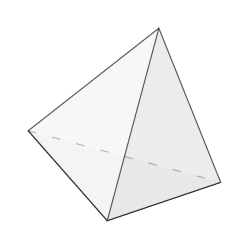
\begin{tikzpicture}
		\coordinate (pic) at (0,0);
		\begin{scope}[shift=(pic), scale=0.8, rotate=-15]
			\coordinate (T) at (pic);
			\coordinate (A) at (-4.5em, -6em);
			\coordinate (B) at (4.5em, -6em);
			\coordinate (C) at (0, -9em);
		\end{scope}
		\draw[fill=gray!10, opacity=0.6] (A) -- (C) -- (B);	% Sisi bawah
		\draw[loosely dashed, opacity=0.6] (A) -- (B);
		\draw[fill=gray!10, opacity=0.6] (T) -- (A) -- (C);	% Sisi kiri
		\draw[fill=gray!25, opacity=0.6] (T) -- (B) -- (C) --cycle;	% Sisi kanan
	\end{tikzpicture} \qquad 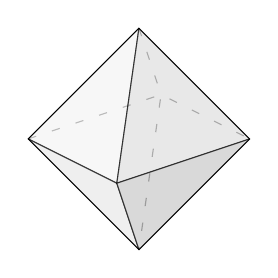
\begin{tikzpicture}
		\coordinate (pic) at (0,0);
		\begin{scope}[shift=(pic), scale=0.8]
			\coordinate (A1) at (pic);
			\coordinate (A2) at (6em, 2em);
			\coordinate (A3) at (10em, 0);
			\coordinate (A4) at (4em, -2em);
			\coordinate (B1) at (5em, 5em);
			\coordinate (B2) at (5em, -5em);
		\end{scope}
		
		\begin{scope}[loosely dashed, opacity=0.6]
			\draw (A1) -- (A2) -- (A3);
			\draw (B1) -- (A2) -- (B2);
		\end{scope}
		\draw[fill=gray!10,opacity=0.6] (A1) -- (A4) -- (B1);
		\draw[fill=gray!20,opacity=0.6] (A1) -- (A4) -- (B2);
		\draw[fill=gray!30,opacity=0.6] (A3) -- (A4) -- (B1);
		\draw[fill=gray!50,opacity=0.6] (A3) -- (A4) -- (B2);
		\draw (B1) -- (A1) -- (B2) -- (A3) --cycle;
	\end{tikzpicture}\end{center}
	dan sebagainya. Dua polihedron disebut kongruen jika keduanya dapat ditumpangtindihkan melalui serangkaian translasi, pencerminan, dan rotasi. Selanjutnya, kita meninjau polihedron hanya hingga kekongruenan. Definisi yang ketat termasuk dalam analisis konveks.
	
	Jika dua polihedron $P, P'$ masing-masing dapat dipotong menjadi banyaknya bagian polihedron kecil yang sama (misalnya dengan pemotongan oleh bidang)
	\[ P = P_1 \cup \ldots \cup P_r, \quad P' = P'_1 \cup \cdots \cup P'_r \]
	sehingga setiap $P_i$ kongruen dengan $P'_i$, maka $P$ dan $P'$ disebut \emph{kongruen-pembedahan}. Sewajarnya, setiap konsep volume polihedron yang masuk akal harus invarian terhadap kongruensi-pembedahan; definisi yang bersesuaian juga tersedia dalam ruang dua dimensi $\mathbb{E}^2$. Untuk mempelajari volume polihedron, Euklides menggunakan apa yang disebut metode penghabisan Eudoksos dalam Buku XI \emph{Unsur-unsur}, suatu pendahulu konsep limit modern. Banyak matematikawan, termasuk Gauss, tidak sepenuhnya puas dan bertanya apakah kesamaan volume dua polihedron dapat diputuskan melalui metode pembedahan elementer. Jawabannya afirmatif dalam dua dimensi (Teorema Bolyai--Gerwien; lihat \cite[Theorem 24.7]{Har00}), sedangkan kasus tiga dimensi merupakan salah satu masalah yang diajukan Hilbert pada Kongres Matematikawan Internasional tahun 1900. Berikut garis besar jawaban negatif M.\ Dehn.
		\begin{enumerate}[(i)]
			\item Untuk setiap rusuk $E$ dari polihedron $P$, tuliskan panjangnya sebagai $\ell(E) \in \R$. Sudut dihedralnya $\angle E \in \R/\pi\Z$ didefinisikan sebagai berikut: pilih suatu bidang $L$ yang melalui titik interior $x$ dari $E$ dan tegak lurus terhadap $E$; sudut dalam poligon $L \cap P$ pada verteks $x$ ialah $\angle E$. Definisikan invarian Dehn dari $P$ sebagai
				\[ \delta(P) := \sum_{E: \text{rusuk}} \ell(E) \otimes \angle E \quad \in A. \]
				% Gambar
				Buktikan bahwa $\delta$ untuk setiap kubus adalah $0$. Buktikan bahwa $\delta$ untuk suatu tetrahedron beraturan dengan panjang rusuk $\ell$ adalah $6\ell \otimes \arccos(\frac{1}{3})$.
			\item Buktikan bahwa jika suatu bidang $\alpha=0$ dalam ruang memotong polihedron $P$ menjadi dua bagian $P = P_+ \cup P_-$, dengan $P_{\pm} := P \cap \{\pm\alpha \geq 0 \}$, maka $\delta(P) = \delta(P_+) + \delta(P_-)$. Dengan demikian, invarian Dehn dipertahankan oleh kongruensi-pembedahan.
				\begin{hint}
					Tinjau rusuk-rusuk baru yang dihasilkan oleh irisan bidang $\alpha=0$; keadaan tipikal mencakup yang berikut.
					\begin{center}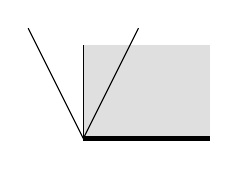
\begin{tikzpicture}[scale=0.7]
						\fill[gray!25] (0,0) rectangle (2.3, 1.7);
						\draw (0,0) -- (-1,2); \draw (0,0) -- (1,2); \draw[ultra thick] (0,0) -- (2.3, 0);
						\draw (0,0) -- (0,1.7);
					\end{tikzpicture} \qquad 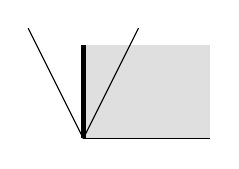
\begin{tikzpicture}[scale=0.7]
						\fill[gray!25] (0,0) rectangle (2.3, 1.7);
						\draw (0,0) -- (-1,2); \draw (0,0) -- (1,2); \draw (0,0) -- (2.3, 0);
						\draw[ultra thick] (0,0) -- (0,1.7);
					\end{tikzpicture} \\ \vspace{2em}
					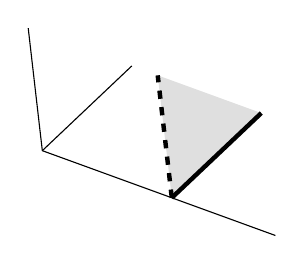
\begin{tikzpicture}[scale=0.7, rotate=-20]
						\fill[gray!25] (0,0) -- (1,2) -- (-1,2) --cycle;
						\draw (-2.5, 0) -- (2, 0);
						\draw[ultra thick] (0,0) -- (1,2); \draw[dashed, ultra thick] (0,0) -- (-1,2);
						\draw (-2.5,0) -- (-3.5, 2); \draw (-2.5,0) -- (-1.5, 2);
					\end{tikzpicture} \qquad 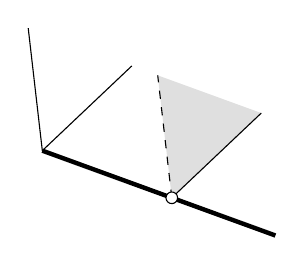
\begin{tikzpicture}[scale=0.7, rotate=-20]
						\fill[gray!25] (0,0) -- (1,2) -- (-1,2) --cycle;
						\draw (0,0) -- (1,2); \draw[dashed] (0,0) -- (-1,2);
						\draw[ultra thick] (0,0) -- (-2.5,0); \draw[ultra thick] (0,0) -- (2,0);
						\filldraw[fill=white] (0,0) circle[radius=3pt];
						\draw (-2.5,0) -- (-3.5, 2); \draw (-2.5,0) -- (-1.5, 2);
					\end{tikzpicture}\end{center}
					Garis tebal menyatakan rusuk baru yang sedang ditinjau, sedangkan daerah berarsir ialah bagian yang dipotong oleh bidang. Gunakan sifat hasil kali tensor untuk memperoleh $\delta(P) = \delta(P_+) + \delta(P_-)$.
				\end{hint}
			\item Buktikan bahwa suatu tetrahedron beraturan tidak mungkin kongruen-pembedahan dengan sebuah kubus, walaupun volumenya dapat sama. \hint{Masalah ini tereduksi menjadi $\arccos(\frac{1}{3}) \notin \Q\pi$. Pembaca dapat mencoba memberikan argumen langsung, atau menerima Proposisi \ref{prop:cos-rationality} yang akan dibuktikan kemudian.}
		\end{enumerate}
		Catatan: J.-P.\ Sydler (1965) membuktikan bahwa dua polihedron $P, P'$ dalam $\mathbb{E}^3$ kongruen-pembedahan jika dan hanya jika keduanya mempunyai volume dan invarian Dehn yang sama.
	\item Buktikan bahwa konstruksi $A \mapsto A^\vee$ dalam Korolari \ref{prop:finite-duality} memberikan suatu ekuivalensi dari kategori grup abelian berhingga $\cate{FinAb}$ ke $\cate{FinAb}^\text{op}$, dan tunjukkan bahwa konstruksi tersebut merupakan fungtor eksak.
	\item Untuk suatu grup abelian bereksponen $A$, buktikan bahwa homomorfisme $\iota_A$ dalam \eqref{eqn:ab-group-duality} bersifat injektif.
		\begin{hint} Kasus grup siklik mudah ditangani. Gunakan sifat bahwa $\Q/\Z$ merupakan modul $\Z$ yang dapat dibagi untuk beralih ke kasus umum. \end{hint}
	\item Lengkapi pembuktian Proposisi \ref{prop:5-lemma-mod} dengan pengejaran diagram.
\end{Exercises}
